\documentclass[12pt]{report}
\usepackage{multicol}
\usepackage[czech]{babel}
\usepackage[dvipsnames]{xcolor}
\usepackage{a4wide}
\usepackage{booktabs}
\usepackage{longtable}
%\usepackage{algorithm}
\usepackage[framemethod=tikz]{mdframed}
\usepackage{threeparttable}
%\usepackage{algorithmic}
\usepackage{amsthm}
\usepackage{amsmath}
%\usepackage{array}
%\usepackage{footnote}
%\usepackage{thmtools}
%\usepackage{mathtools}
%\usepackage{tikz}
\usepackage{tkz-graph}
\usepackage{tkz-berge}
\usetikzlibrary{shapes.geometric}
\usetikzlibrary{arrows}
\usepackage{amsmath, amssymb, amsfonts}
\usepackage[all]{xypic}
\usepackage{graphicx}
\usepackage{fancyhdr}
\usepackage{caption}
\usepackage{thmtools}
\usepackage{mathalfa}
\usepackage{verse}
\usepackage{extarrows}
\usepackage{enumerate}
\renewcommand{\labelenumi}{(\roman{enumi})} 
\usepackage{tabularx}
\usepackage{wrapfig}
\usepackage{color}
\usepackage{array}
\usepackage{textcomp}
\usepackage{siunitx}
\usepackage{tikz-cd}
\usetikzlibrary{arrows}
\usepackage{pgfplots}
\usetikzlibrary{babel}
\usepackage{epsfig}
\PassOptionsToPackage{hyphens}{url}
\usepackage{hyperref}[hyperfootnotes=false]
\hypersetup{colorlinks,
citecolor=RoyalBlue
}
\usepackage{url}
\usepackage{tabularx}
\usetikzlibrary{intersections}

%\usepackage{tkz-euclide} 


%\usepackage[metapost, mplabels,truebbox,clip]{mfpic}
%\allowdisplaybreaks
%\usepackage{scrextend}
\makeatletter
\newcommand\figcaption{\def\@captype{figure}\caption}
\makeatother

\renewcommand{\sectionmark}[1]{ \markright{-- \thesection.\ #1}{}}

\fancypagestyle{plain}{%
\fancyhf{}
\lhead[L]{}
\chead{}
\rhead[R]{\nouppercase\leftmark}
\lfoot{}
\cfoot{}
\rfoot{\thepage}
\renewcommand{\headrulewidth}{0.4pt}}

\pagestyle{fancy}
\fancyhf{}
\lhead[L]{}
\chead{}
\rhead[R]{\nouppercase\leftmark}
\lfoot{}
\cfoot{}
\rfoot{\thepage}

\DeclareMathOperator{\Tr}{Tr}
\DeclareMathOperator{\N}{N}
\DeclareMathOperator{\End}{End}
\DeclareMathOperator{\id}{id}
\DeclareMathOperator{\Ell}{Ell}
\DeclareMathOperator{\ord}{ord}
\DeclareMathOperator{\AG}{AG}
\DeclareMathOperator{\HG}{HG}
\DeclareMathOperator{\AH}{AH}
\usepackage{tkz-euclide}  

\begin{document}

\newcommand{\ZZ}{{\mathbb{Z}}}
\newcommand{\cyc}[1]{{\langle #1 \rangle}}


\newtheorem{veta}{Věta}[section]
%\newtheorem{definice}{Definice}[section]
%\newtheorem{dusledek}{Důsledek}[section]
%\newtheorem{lemma}{Lemma}[section]


\theoremstyle{de}
\newtheorem{de}{Definition}[section]
\newtheorem{dusledek}[veta]{Důsledek}
\newtheorem{lemma}[veta]{Lemma}
\newtheorem{domnenka}[veta]{Domněnka}
\newtheorem*{lemma*}{Lemma}

\theoremstyle{definition}
\newtheorem{priklad}[veta]{Příklad}
\newtheorem{definice}[veta]{Definice}
\newtheorem{problem}[veta]{Problém}
\newtheorem{znaceni}[veta]{Značení}
\newtheorem*{umluva}{Úmluva}
\newtheorem*{poznamka}{Poznámka}
\newtheorem{dfn}[veta]{Definition}

%\newmdtheoremenv[linewidth=1pt,roundcorner=4pt]{theo}{Věta}
%declaretheorem[
%  shaded={rulecolor=black, rulewidth=2pt},
%  name=Věta,
%]{theo}

%\floatname{algorithm}{Algoritmus}

\setlength{\parindent}{2ex}
\setlength{\emergencystretch}{3em}


\begin{titlepage}
{
\centering
\LARGE \textbf{STŘEDOŠKOLSKÁ ODBORNÁ ČINNOST}\\
\Large\textbf{Obor č. 1: Matematika a statistika}\\
\vspace{6cm}
\LARGE\textbf{Medúzy a posloupnosti průměrů}\\
}
\vspace{1cm}
  \begin{center}
 \begin{tikzpicture}[node distance=2cm]
\def\s{1.1}
\def\l{3mm}
\def\w{1mm}
%\draw[line width=.5pt,black,fill=yellow] (0:4cm) circle (3pt);

%\draw[line width=.5pt,black,fill=yellow] (60:4cm) circle (3pt);
%\draw[line width=.5pt,black,fill=yellow] (120:4cm) circle (3pt);
%\draw[line width=.5pt,black,fill=yellow] (180:4cm) circle (3pt);
%\draw[line width=.5pt,black,fill=yellow] (240:4cm) circle (3pt);
%\draw[line width=.5pt,black,fill=yellow] (300:4cm) circle (3pt);
%\draw[line width=.5pt,black,fill=yellow] (0:8cm) circle (3pt);
 
%\draw[line width=.5pt,black,fill=yellow] (60:8cm) circle (3pt);
%\draw[line width=.5pt,black,fill=yellow] (120:8cm) circle (3pt);
%\draw[line width=.5pt,black,fill=yellow] (180:8cm) circle (3pt);
%\draw[line width=.5pt,black,fill=yellow] (240:8cm) circle (3pt);
%\draw[line width=.5pt,black,fill=yellow] (300:8cm) circle (3pt);
\node [draw,black,fill=yellow, circle,inner sep=2pt, scale=\s, name=c1]      at (0:1.5cm){};
\node [draw,black,fill=yellow, circle,inner sep=2pt, scale=\s, name=c2]      at (360/10:1.5cm){};
\node [draw,black,fill=yellow, circle,inner sep=2pt, scale=\s, name=c3]      at (2*360/10:1.5cm){};
\node [draw,black,fill=yellow, circle,inner sep=2pt, scale=\s,  name=c4]      at (3*360/10:1.5cm){};
\node [draw,black,fill=yellow, circle,inner sep=2pt, scale=\s,  name=c5]      at (4*360/10:1.5cm){};
\node [draw,black,fill=yellow, circle,inner sep=2pt, scale=\s, name=c6]      at (5*360/10:1.5cm){};
\node [draw,black,fill=yellow, circle,inner sep=2pt, scale=\s, name=c7]      at (6*360/10:1.5cm){};
\node [draw,black,fill=yellow, circle,inner sep=2pt, scale=\s, name=c8]      at (7*360/10:1.5cm){};
\node [draw,black,fill=yellow, circle,inner sep=2pt, scale=\s,  name=c9]      at (8*360/10:1.5cm){};
\node [draw,black,fill=yellow, circle,inner sep=2pt, scale=\s,  name=c10]      at (9*360/10:1.5cm){};
\node [draw,black,fill=yellow, circle,inner sep=2pt, scale=\s, name=b1]      at (0:3cm){};
\node [draw,black,fill=yellow, circle,inner sep=2pt, scale=\s, name=b2]      at (360/10:3cm){};
\node [draw,black,fill=yellow, circle,inner sep=2pt, scale=\s, name=b3]      at (2*360/10:3cm){};
\node [draw,black,fill=yellow, circle,inner sep=2pt, scale=\s,  name=b4]      at (3*360/10:3cm){};
\node [draw,black,fill=yellow, circle,inner sep=2pt, scale=\s,  name=b5]      at (4*360/10:3cm){};
\node [draw,black,fill=yellow, circle,inner sep=2pt, scale=\s, name=b6]      at (5*360/10:3cm){};
\node [draw,black,fill=yellow, circle,inner sep=2pt, scale=\s, name=b7]      at (6*360/10:3cm){};
\node [draw,black,fill=yellow, circle,inner sep=2pt, scale=\s, name=b8]      at (7*360/10:3cm){};
\node [draw,black,fill=yellow, circle,inner sep=2pt, scale=\s,  name=b9]      at (8*360/10:3cm){};
\node [draw,black,fill=yellow, circle,inner sep=2pt, scale=\s,  name=b10]      at (9*360/10:3cm){};
\draw [-{Stealth[length=\l, width=\w]}](c2) -- (c1);
\draw [-{Stealth[length=\l, width=\w]}](c3) -- (c2);
\draw [-{Stealth[length=\l, width=\w]}](c4) -- (c3);
\draw [-{Stealth[length=\l, width=\w]}](c5) -- (c4);
\draw [-{Stealth[length=\l, width=\w]}](c6) -- (c5);
\draw [-{Stealth[length=\l, width=\w]}](c7) -- (c6);
\draw [-{Stealth[length=\l, width=\w]}](c8) -- (c7);
\draw [-{Stealth[length=\l, width=\w]}](c9) -- (c8);
\draw [-{Stealth[length=\l, width=\w]}](c10) -- (c9);
\draw [-{Stealth[length=\l, width=\w]}](c1) -- (c10);
\draw [-{Stealth[length=\l, width=\w]}](b1) -- (c1);
\draw [-{Stealth[length=\l, width=\w]}](b2) -- (c2);
\draw [-{Stealth[length=\l, width=\w]}](b3) -- (c3);
\draw [-{Stealth[length=\l, width=\w]}](b4) -- (c4);
\draw [-{Stealth[length=\l, width=\w]}](b5) -- (c5);
\draw [-{Stealth[length=\l, width=\w]}](b6) -- (c6);
\draw [-{Stealth[length=\l, width=\w]}](b7) -- (c7);
\draw [-{Stealth[length=\l, width=\w]}](b8) -- (c8);
\draw [-{Stealth[length=\l, width=\w]}](b9) -- (c9);
\draw [-{Stealth[length=\l, width=\w]}](b10) -- (c10);
%\node[text width=3cm] at (300:4cm) {$(1,2)$};
%\node[text width=3cm] at (0:4cm) {$(5,3)$};
\end{tikzpicture}

\end{center}

\vspace{3cm}
{\noindent\large\bfseries Zdeněk Pezlar\\ 
	\large\bfseries Jihomoravský kraj\\ }
\center\large Brno 2022
	
\end{titlepage}

\begin{titlepage}
{
\centering
\LARGE \textbf{STŘEDOŠKOLSKÁ ODBORNÁ ČINNOST}\\
\Large\textbf{Obor č. 1: Matematika a statistika}\\
\vspace{6cm}
\LARGE\textbf{Medúzy a posloupnosti průměrů}\\
\vspace{1cm}
\LARGE\textbf{On Jellyfish and Sequences of Means}\\
}
\vspace{6cm}
{\noindent\large\bfseries Autor: Zdeněk Pezlar\\ 
	\large\bfseries Škola: Gymnázium Brno, třída Kapitána Jaroše, p. o.\\
    \large\bfseries Kraj: Jihomoravský \\
	\large\bfseries Vedoucí: Mgr. Vojtěch Suchánek
	}
	

\end{titlepage}

\newpage
\thispagestyle{empty}
\vspace*{14cm}
\subsubsection*{Prohlášení}

Prohlašuji, že jsem svou práci SOČ vypracoval samostatně a použil jsem pouze prameny a literaturu uvedené v seznamu bibliografických záznamů.
Prohlašuji, že tištěná verze a elektronická verze soutěžní práce SOČ jsou shodné. 
Nemám závažný důvod proti zpřístupňování této práce v souladu se zákonem č. 121/2000 Sb., o právu autorském, o~právech souvisejících s právem autorským a o změně některých zákonů (autorský zákon) v~platném znění. \\[1cm]
V Brně dne: \dotfill \ \ \ \ \ \  Podpis: \dotfill

\newpage
\thispagestyle{empty}
\begin{center}

\includegraphics[width=0.35\textwidth]{podpora_soc-horizontalni.png}
\end{center}
\vspace*{1.5cm}
\begin{center}

\includegraphics[width=0.45\textwidth]{logo_JMK_pruhledne.png}
\end{center}
\vspace*{2.2cm}
\begin{center}

\includegraphics[width=0.35\textwidth]{jcmm-logotype-positive1.png}
\end{center}
\vspace*{5.5cm}
\subsection*{Poděkování}
Mé díky patří všem lidem, kteří mi pomohli k dokončení práce. Zejména děkuji Vojtovi Suchánkovi za jeho ochotu vzít vedení práce a jeho nekončící trpělivost při opravách práce a konzultacích nápadů. Dále děkuji přátelům Richardu Blažkovi za podnětné debaty, které práci posunovaly, a dále Kubovi Devátovi, Martinu Dominikovi, Vojtovi Obořilovi, Danu Pravcovi a Vojtovi Stránskému za jejich pomoc při jazykových opravách. Konečně děkuji Verče za její neustálou podporu. 


\newpage
\thispagestyle{empty}
\subsection*{Abstrakt}
V práci podáváme první systematický úvod do posloupnosti průměrů nad konečnými tělesy. Nejprve se zaobíráme posloupnostmi průměrů nad reálnými čísly, jejichž studium se táhne až ke Karlu Gaussovi. V následující kapitole navazujeme na aktuální článek \cite{Meduza} a studujeme tři posloupnosti průměrů nad konečnými tělesy. Nejprve zkoumáme posloupnost danou aritmetickým a geometrickým průměrem a experimentálně ověřujeme odhady podané v~\cite{Meduza}. Později v práci tuto posloupnost propojíme s teorií isogenií eliptických křivek. Hlavní přínos práce spočívá ve formulaci dvou nové posloupnosti průměrů a jejich následného studia. Zejména v závěru práce propojíme posloupnosti dané aritmetickým a harmonickým průměrem se singulární eliptickou křivkou, díky čemuž kompletně určíme strukturu grafů generovaných aritmetickým a harmonickým průměrem.



\subsection*{Klíčová slova}
Aritmeticko-geometrický průměr, Aritmeticko-harmonický průměr, Harmonicko-geometrický průměr, eliptické křivky, isogenie, grupa tříd ideálů, Vulkány, Medúzy


\vspace*{4cm}

\subsection*{Abstract}


\subsection*{Key words}
Arithmetic-Geometric Mean, Arithmetic-Harmonic Mean, Harmonic-Geometric Mean, Elliptic Curves, Isogeny, Ideal Class Group, Volcanoes, Jellyfish




{
\hypersetup{linkcolor=black}
\tableofcontents
}
\thispagestyle{empty}

\chapter*{Úvod}
\addcontentsline{toc}{chapter}{Úvod}
\markboth{Úvod}{}


S aritmetickým a geometrickým průměrem se setkáváme už od základní školy. Pro libovolnou dvojici $(a,b)$ kladných čísel můžeme spočítat tuto dvojici průměrů jako:
$$\left(\frac{a+b}{2}, \sqrt{ab} \right).$$

Tato práce staví na jednoduché myšlence -- na opakované aplikaci těchto průměrů. Přesněji definujme posloupnost $((a_n,b_n))_{n=0}^{\infty}$ s počátečním členem $(a_0,b_0) = (a,b)$ a pro každé nezáporné $n$ platí:
$$\left(a_{n+1},b_{n+1} \right) = \left( \frac{a_n+b_n}{2}, \sqrt{a_n b_n} \right).$$

Velcí matematici jako Gauss, Legendre a Lagrange tuto tzv. \textit{AG posloupností} studovali. Proč se však ti nejlepší z nejlepších zabývali tak zdánlivě jednoduchou posloupností? Carl Friedrich Gauss ukázal, že AG posloupnost vždy konverguje ke společné hodnotě. O co víc, posloupnost má kořeny hluboko v oblasti eliptických integrálů. O tomto propojení napsal:
\begin{center}
\begin{verse}
\setverselinenums{1}{3}
\textit{\uv{This [...] will surely open up an entirely new field of analysis.}}
\end{verse}
\end{center}
Přes následující století různí autoři studovali AG posloupnost a ukázali mj., že ji lze využít k rychlým výpočtů elementárních funkcí jako je $e^x$ či $\arcsin(x)$, ale i že je spojená s \textit{modulárními funkcemi} a \textit{modulárními formami}. Gauss měl proto pravdu.

V naší práci se na posloupnost díváme v jiném světle, konkrétně v oboru konečných těles. Jelikož pracujeme v konečném oboru je AG posloupnost vždy periodická, můžeme se proto zabývat orientovanými grafy generovanými AG posloupností. Všechny komponenty slabé souvislosti, které získáme, mají typický tvar cyklu, kde ke každému prvku cyklu je připojena jediná hrana. Takový graf nazveme \textit{medúzou}.

Pokud se podíváme na medúzy obsažené v takových grafech pro různá $p$ tak zjistíme, že se jejich počty i velikosti chovají zdánlivě náhodně. Pomocí efektivní implementace v jazyku Sage poskytujeme rozsáhlé grafy hodnot spojených s AG posloupností. Dále experimentálně ověřujeme a navrhujeme odhady položené ve článku \cite{Meduza} a zavádíme nové struktury, které nám pomohou ve studiu posloupnosti.

%Ukážeme, že tyto medúzy jsou spojené s grafy eliptických křivek a setkáme se s tzv. \textit{grupou tříd ideálů}. Výpočetně ověříme jisté odhady položené v \cite{Meduza} a podíváme se podrobně na hodnoty spojené s těmito grafy, nejpodstatněji na počet komponent souvislosti v tomto grafu.

\begin{figure}[!h]
\begin{center}
 \begin{tikzpicture}[node distance=2cm]
\def\s{0.7}
\def\l{2mm}
\def\w{1mm}
%\draw[line width=.5pt,black,fill=yellow] (0:4cm) circle (3pt);

%\draw[line width=.5pt,black,fill=yellow] (60:4cm) circle (3pt);
%\draw[line width=.5pt,black,fill=yellow] (120:4cm) circle (3pt);
%\draw[line width=.5pt,black,fill=yellow] (180:4cm) circle (3pt);
%\draw[line width=.5pt,black,fill=yellow] (240:4cm) circle (3pt);
%\draw[line width=.5pt,black,fill=yellow] (300:4cm) circle (3pt);
%\draw[line width=.5pt,black,fill=yellow] (0:8cm) circle (3pt);
 
%\draw[line width=.5pt,black,fill=yellow] (60:8cm) circle (3pt);
%\draw[line width=.5pt,black,fill=yellow] (120:8cm) circle (3pt);
%\draw[line width=.5pt,black,fill=yellow] (180:8cm) circle (3pt);
%\draw[line width=.5pt,black,fill=yellow] (240:8cm) circle (3pt);
%\draw[line width=.5pt,black,fill=yellow] (300:8cm) circle (3pt);
\node [draw,black,fill=yellow, circle,inner sep=2pt, scale=\s, name=c1]      at (0:1.25cm) {};
\node [draw,black,fill=yellow, circle,inner sep=2pt, scale=\s, name=c2]      at (60:1.25cm) {};
\node [draw,black,fill=yellow, circle,inner sep=2pt, scale=\s, name=c3]      at (120:1.25cm) {};
\node [draw,black,fill=yellow, circle,inner sep=2pt, scale=\s,  name=c4]      at (180:1.25cm) {};
\node [draw,black,fill=yellow, circle,inner sep=2pt, scale=\s,  name=c5]      at (240:1.25cm) {};
\node [draw,black,fill=yellow, circle,inner sep=2pt, scale=\s,  name=c6]      at (300:1.25cm) {};
\node [draw,black,fill=yellow, circle,inner sep=2pt, scale=\s,  name=b1]      at (0:2.5cm) {};
\node [draw,black,fill=yellow, circle,inner sep=2pt, scale=\s,  name=b2]      at (60:2.5cm) {};
\node [draw,black,fill=yellow, circle,inner sep=2pt, scale=\s,  name=b3]      at (120:2.5cm) {};
\node [draw,black,fill=yellow, circle,inner sep=2pt, scale=\s,  name=b4]      at (180:2.5cm) {};
\node [draw,black,fill=yellow, circle,inner sep=2pt, scale=\s,  name=b5]      at (240:2.5cm) {};
\node [draw,black,fill=yellow, circle,inner sep=2pt, scale=\s,  name=b6]      at (300:2.5cm) {};
\draw [-{Stealth[length=\l, width=\w]}](c2) -- (c1);
\draw [-{Stealth[length=\l, width=\w]}](c3) -- (c2);
\draw [-{Stealth[length=\l, width=\w]}](c4) -- (c3);
\draw [-{Stealth[length=\l, width=\w]}](c5) -- (c4);
\draw [-{Stealth[length=\l, width=\w]}](c6) -- (c5);
\draw [-{Stealth[length=\l, width=\w]}](c1) -- (c6);
\draw [-{Stealth[length=\l, width=\w]}](b1) -- (c1);
\draw [-{Stealth[length=\l, width=\w]}](b2) -- (c2);
\draw [-{Stealth[length=\l, width=\w]}](b3) -- (c3);
\draw [-{Stealth[length=\l, width=\w]}](b4) -- (c4);
\draw [-{Stealth[length=\l, width=\w]}](b5) -- (c5);
\draw [-{Stealth[length=\l, width=\w]}](b6) -- (c6);
%\node[text width=3cm] at (300:4cm) {$(1,2)$};
%\node[text width=3cm] at (0:4cm) {$(5,3)$};
\end{tikzpicture}


\end{center}
\end{figure}

Ve čtvrté kapitole osvětlíme sporadické chování AG posloupnosti nad konečnými tělesy. Ukážeme totiž, že posloupnost popisuje tzv. \textit{vulkány} eliptických křivek nad konečnými tělesy a že velikosti medúz jsou úzce spojené s grupou tříd ideálů jistých imaginárních kvadratických těles.

Hlavní přínos práce spadá do kapitol \ref{AH} a \ref{5}. Ve třetí kapitole definujeme předtím nestudovanou AH posloupnost nad konečným tělesem a teoreticky i experimentálně určíme jejich vlastnosti, zejména pozoruhodné jsou tvary grafů, které generuje. Krom medúz totiž grafy udávající AH posloupnost tvoří i hlubší vulkány a pro některá tělesa přesně určíme jejich hloubku. Vyvrcholení nastane v páté kapitole, kde ukážeme, že posloupnost můžeme popsat pomocí skalárních násobků na jisté singulární eliptické křivce. Díky tomuto propojení určíme plnou strukturu komponent souvislosti a poskytneme netriviální odhady na jejich počty.

%Na tomto místě končí článek \cite{Meduza}, na který práce odpovídá. Hlavní přínos práce spočívá v definici a studiu podobných posloupností užívajících průměry nad konečnými tělesy. Konkrétně se podíváme na posloupnosti s harmonickým a geometrickým, resp. aritmetickým a harmonickým průměrem. Ukážeme, že první z nich je s $AG$ posloupností shodná, druhá se však podstatně liší. Grafy tzv. \textit{AH posloupnosti} charakterizujeme a ukážeme, že jsou ještě zajímavější, než pouhé medúzy. Ve finální části práce i tuto posloupnost propojíme s teorií dynamických systémů a eliptických křivek, což nám též dá netriviální odhady na počty komponent souvislosti.

\chapter{AG posloupnost nad reálnými čísly}


Nejprve se budeme zabývat posloupností dvojic kladných reálných čísel, přičemž každá další je tvořena aritmetickým a geometrickým průměrem té předchozí. I~v~tomto jednoduchém prostředí narazíme na posloupnost v místech, kde bychom vůbec nehledali.

\section{Seznámení s posloupností}


\begin{definice}
Ať $a \geqslant b$ jsou dvě kladná reálná čísla. Pak definujme \textit{AG posloupnost} jako posloupnost $((a_n,b_n))_{n=0}^{\infty}$ tak, že $(a_0,b_0) = (a,b)$ a:
$$\left(a_{n+1},b_{n+1} \right) = \left(\frac{a_n+b_n}{2}, \sqrt{a_n b_n} \right).$$
Jednotlivá čísla $a_i$ a $b_i$ nazveme \textit{složkami} prvku $(a_i,b_i)$ této posloupnosti.
\end{definice}

Toto značení ponechme po zbytek sekce. První vlastnosti, které si všimněme, je monotónnost obou složek $(a_n)_{n=0}^{\infty}$ a $(b_n)_{n=0}^{\infty}$. Z $AG$ nerovnosti je totiž platné $a_n \geqslant b_n$ a~proto:
$$ b_{n+1} = \sqrt{a_n b_n} \geqslant b_n,$$
posloupnost $(b_n)_{n=0}^{\infty}$ je proto rostoucí (pokud $a_0 \neq b_0$, tak ostře rostoucí). Obdobně  můžeme psát:
$$a_{n+1} = \frac{a_n+b_n}{2} \leqslant a_n,$$
posloupnost $(a_n)_{n=0}^{\infty}$ je tedy naopak klesající. Protože aritmetický a geometrický průměr dvou čísel leží mezi nimi, jsou obě posloupnosti shora svírané prvkem $a$ a zdola $b$. Libovolná ohraničená monotónní posloupnost konverguje, víme tedy, že obě posloupnosti $(a_n)_{n=0}^{\infty}$ a~$(b_n)_{n=0}^{\infty}$ konvergují. Abychom získali nějakou představu o jejich limitách, ukážeme si pár příkladů.

\begin{priklad}\label{pr1}
Pokud si zvolíme $a=b=5$, tak jsou obě hodnoty konstantní, to příliš zajímavě není. Zvolme si tedy například trochu záživnější dvojici $a = 8, b = 2$. Pak můžeme psát:


\begin{longtable}[H]{>{\raggedright\arraybackslash}p{0.3\linewidth}p{0.202\linewidth}}
\toprule
$a_i$ & $b_i$\\
\midrule
$8$ & \noindent $2$\\
$5$ & \noindent $4$\\
$ 4.5$ & $4.472135955000\dots$\\
$4.486067977500\dots$ & $4.486046343664\dots$\\
$4.486057160582\dots$ & $4.486057160569\dots$\\ 
$4.486057160575\dots$ & $4.486057160575\dots$\\
$4.486057160575\dots$ & $4.486057160575\dots$\\
$4.486057160575\dots$ & $4.486057160575\dots$\\
\vdots & \vdots\\
\bottomrule 
\end{longtable}




\begin{figure}[h]
\centering
\begin{minipage}{.5\textwidth}
  \centering
  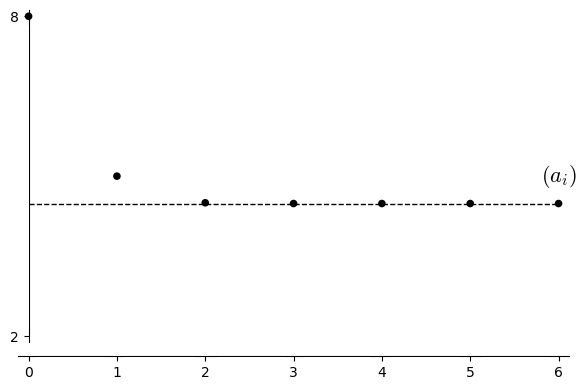
\includegraphics[width=.9\linewidth]{Ai2.png}
  \captionof{figure}{složka $(a_i)$}
  \label{složka $(a_i)$}
\end{minipage}%
\begin{minipage}{.5\textwidth}
  \centering
  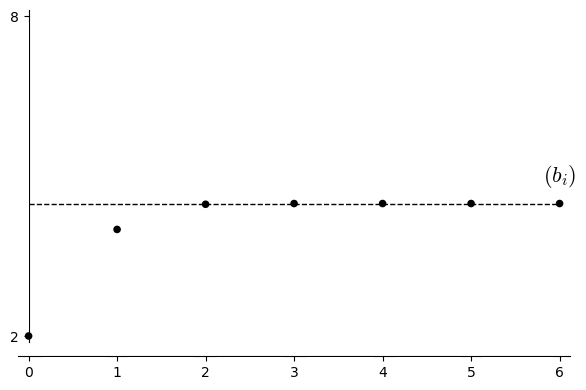
\includegraphics[width=.9\linewidth]{Bi2.png}
  \captionof{figure}{složka $(b_i)$}
  \label{složka $(b_i)$}
\end{minipage}
\end{figure}
V tomto případě prvky $AG$ posloupnosti zdárně konvergují ke společné hodnotě. Spočítejme si ještě pro jistotu jednu posloupnost, tentokrát pro dvojici $a=\sqrt{2}$ a $b=1$.

\begin{longtable}[H]{>{\raggedright\arraybackslash}p{0.3\linewidth}p{0.202\linewidth}}
\toprule
$a_i$ & $b_i$\\
\midrule
$1.414213562373\dots$ & $1$\\
$1.207106781187\dots$ & $1.189207115003\dots$\\
$1.198156948095\dots$ & $1.198123521493\dots$\\
$1.198140234794\dots$ & $1.198140234677\dots$\\
$1.198140234736\dots$ & $1.198140234736\dots$\\
$1.198140234736\dots$&  $1.198140234736\dots$\\
$1.198140234736\dots$&  $1.198140234736\dots$\\
\vdots & \vdots\\
\bottomrule 
\end{longtable}
\end{priklad}

Složky $AG$ posloupnosti vždy konvergují ke společné hodnotě. Na příkladu \ref{pr1} vidíme, že konvergují velmi rychle, jak ale takovou rychlost můžeme měřit?
\begin{definice}
Ať $(x_n)_{n=0}^{\infty}$ je konvergentní posloupnost. Poté \textit{řád konvergence} $\sigma$ této posloupnosti k limitě $L$ je číslo splňující pro všechna $n \in \mathbb{N}$ a nějakou konstantu $C$:
$$\frac{\vert x_{n+1} - L \vert}{\vert x_n - L \vert ^ \sigma} \leqslant C.$$
Pro $\sigma = 2$ získáme \textit{kvadraticky konvergentní posloupnost}. 
\end{definice}

U kvadraticky konvergující posloupnosti se tak v~každém dalším kroku se obě čísla \textit{přibližně} rovnají limitě na dvakrát více desetinných míst. Na druhé posloupnosti zmíněné v příkladu \ref{pr1} pozorujeme, že třetí iterace $AG$ posloupnosti čísel $2$ a $8$ se s limitou shoduje už na čtyřech desetinných místech. Ta následující dokonce na desíti. Opravdu, $AG$ posloupnost konverguje a konverguje kvadraticky.

\begin{veta}\label{conv}
Ať $((a_n,b_n))_{n=0} ^{\infty}$ je $AG$ posloupnost. Pak limity složek $(a_n)_{n=0}^{\infty}$ a $(b_n)_{n=0}^{\infty}$ pro $n$ jdoucí do nekonečna existují a jsou si navzájem rovné. Navíc tyto složky konvergují ke společné limitě kvadraticky.
\end{veta}


\noindent \textit{Důkaz.} Existenci limit složek jsme si ukázali výše. Jelikož platí:
$$ 0 \leqslant a_n - b_n  =  2 \left( a_n - \frac{a_n+ b_n}{2} \right) = 2 ( a_{n} - a_{n+1} )$$
a navíc $\lim_{n \rightarrow \infty} (a_n - a_{n+1}) = 0$, platí $\lim_{n \rightarrow \infty} (a_n - b_n) = 0$. Limity posloupností $(a_n)$ a $(b_n)$ jsou proto shodné.

Zaveďme nyní pomocné posloupnosti $(x_n)_{n=0}^{\infty}$ a $(\varepsilon_i)_{n=0}^{\infty}$ splňující $x_i = \frac{a_i}{b_i} = 1 + \varepsilon_i$ pro každé $i$. Chceme ukázat, že posloupnost $(x_n)$ konverguje kvadraticky k $1$. Platí $\varepsilon_i \geqslant 0$ pro každé $i$. Pak pro libovolné $n$ platí:
\begin{align*}
x_{n+1} = \frac{a_n+b_n}{2 \sqrt{a_n b_n}} &= \frac{\sqrt{\frac{a_n}{b_n}} + \sqrt{\frac{b_n}{a_n}}}{2} = \frac{\sqrt{x_n}+\frac{1}{\sqrt{x_n}}}{2}\\
x_{n+1} &=\frac{\sqrt{x_n}+\frac{1}{\sqrt{x_n}}}{2}\\
1+\varepsilon_{n+1}  &= \frac{\sqrt{1+\varepsilon_n} + \frac{1}{\sqrt{1+\varepsilon_n}}}{2}.
\end{align*}
Taylorova řada funkce $\sqrt{x}$ v bodě $1$ je $1+\frac{x}{2} - \frac{x^2}{8} + O(x^3)$ a Taylorova řada funkce $\sqrt{x}^{-1}$ je $1-\frac{x}{2}+\frac{3 x^2}{8} + O(x^3)$. Proto pro $n$ dostatečně velké a tedy $\varepsilon_n$ dostatečně malé platí:
$$1+\varepsilon_{n+1}  = 1+\frac{\varepsilon_n ^2}{8} + O(\varepsilon_n ^3),$$ 
řád konvergence $\frac{a_i}{b_i} \rightarrow 1$ je tedy kvadratický. \hfill $\square$\\


\begin{definice}
Ať $((a_n,b_n))_{n=0}^{\infty}$ je $AG$ posloupnost. Společnou limitu složek $(a_n),(b_n)$ nazvěme \textit{aritmeticko-geometrickým průměrem}, zkráceně \textit{AG průměrem}, čísel $a,b$. Toto číslo značme $\AG(a,b)$.
\end{definice}


Následující věta shrnuje základní vlastnosti $AG$ průměru.


\begin{veta}\label{zkjb}
Mějme $a>b,k \in \mathbb{R}^{+}$. Pro $AG$ průměr platí:
\begin{enumerate}
\item $\AG(a,a) = a$,
\item $\AG(ka,kb) = k \AG (a,b)$,\label{zkjb2}
\item $\AG(a,b) = \AG(a_1,b_1) = \AG(a_2,b_2) = \dots$,
\item $\AG(1-x,1+x) = \AG(a,b)$, kde $x = \frac{1}{a} \sqrt{a^2 - b^2}$.\footnote[1]{Tato vlastnost nám přijde vhod v následující sekci.}
\end{enumerate}
\end{veta}

Prozatím může vypadat, že $AG$ posloupnost leží v uzavřeném ostrůvku vzdálená od jiných oblastí matematiky. Toto zdání však nemůže být dál od pravdy. Zamysleme se nad samotným $AG$ průměrem. Pro čísla $2$ a $8$ získáváme průměr $4.48605716\dots$. Jak takové číslo určit uzavřeně? K nalezení odpovědi budeme muset nakouknout do sféry tzv. \uv{eliptických integrálů}.
\section{Eliptické integrály}

\begin{definice}
Definujme \textit{eliptický integrál prvního druhu} jako následující určitý integrál:
\begin{equation*}
K(t) := \int_{0}^{\pi/2} \frac{d \theta}{\sqrt{1 - t^2 \sin^2 \theta}}.
\end{equation*}
\end{definice}

Tento integrál a tzv. eliptický integrál \uv{druhého druhu} mají mnoho využití, například v počítání délky oblouku na elipse, ve světě fyziky zase například pomáhají najít periodu kmitu kyvadla \cite{Crawford}.

My eliptické integrály zmiňujeme, jelikož jsou intimně spojené s $AG$ posloupností, umožní nám totiž přesně vyjádřit hodnotu $AG(a,b)$. Mladý Karl Friedrich Gauss si již ve svých dvaadvaceti letech do svého deníku poznačil, že se hodnoty:
$$\frac{1}{\AG\left(1,\frac{\sqrt{2}}{2}\right)} \qquad  \text{a} \qquad \frac{2}{\pi} K\left(\frac{\sqrt{2}}{2} \right)$$
shodují na $11$ desetinných místech \cite{Pi}. O trochu později dokázal obecný vztah, který tyto dva koncepty spojuje.
\begin{veta} (Gauss)\label{Ga}
Pro $x<1$ platí:
\begin{equation}\label{el}
\frac{\pi}{2} \cdot \frac{1}{\AG(1,x)} = K\left(\sqrt{1 - x^2}\right)
\end{equation}
\end{veta}

Nyní nepatrně pozměňme integrál napravo, abychom mohli obecně popsat číslo $\AG(a,b)$. Definujme:
$$I(a,b) := \int_{0}^{\pi/2} \frac{d \theta}{\sqrt{a^2 \cos ^2 \theta + b^2 \sin ^2 \theta}}. $$
Pomocí goniometrické jedničky $\sin^2 \theta + \cos^2 \theta = 1$ vidíme, že platí vztah:
$$I(a,b) = \frac{1}{a} K(x),$$ kde $x =\frac{1}{a} \sqrt{a^2-b^2}$. Takové $x$ jsme už ale někde viděli, konkrétně v části $iv)$ věty \ref{zkjb}. Gaussovu větu poté můžeme díky části $ii)$ věty \ref{zkjb} přepsat na:
\begin{veta}\label{Ia}
$$\frac{\pi}{2} \frac{1}{\AG(a,b)} = I(a,b).$$
\end{veta}


\begin{priklad}
Pojďme ověřit, že opravdu věta \ref{Ia} platí. Nejprve pokud zvolíme $a=b$, tak máme:
$$I(a,a) = \int_{0}^{\pi/2} \frac{d \theta}{a} = \frac{\pi}{2 a} = \frac{\pi}{2 \AG(a,a)}.$$
Podívejme se nyní znovu na volbu $a= 8$ a $b=2$. Určíme přibližně hodnotu $I(8,2)$ pomocí Simpsonova pravidla pro numerickou integraci:
\begin{align*}
I(8,2) \cdot \frac{2}{\pi} &= \int_{0}^{\pi/2} \frac{d \theta}{\sqrt{64 \cos ^2 \theta + 4 \sin ^2 \theta}} \cdot \frac{2}{\pi}\\
&\approx \frac{\pi}{12} \cdot \left( \frac{1}{\sqrt{64 \cos ^2 0 + 4 \sin ^2 0}} + \frac{4}{\sqrt{64 \cos ^2 \pi/4 + 4 \sin ^2 \pi/4}} + \frac{1}{\sqrt{64 \cos ^2 \pi/2 + 4 \sin ^2 \pi/2}} \right) \cdot \frac{2}{\pi}\\
&= \frac{1}{6} \cdot \left( \frac{1}{8} +\frac{4}{\sqrt{32+2}} + \frac{1}{2}  \right) = 0.2184990567617\dots.
\end{align*}
Převrácená hodnota tohoto čísla je:
$$\frac{\pi}{2} \cdot \frac{1}{I(8,2)} \approx 4.576678795876\dots,$$
což při porovnání s $\AG(8,2) = 4.486057160575\dots$ není daleko od opravdové hodnoty. Obdobně můžeme ověřit: 
\begin{align*}
I\left(\sqrt{2},1\right) \cdot \frac{2}{\pi} &= \int_{0}^{\pi/2} \frac{d \theta}{\sqrt{ 2 \cos ^2 \theta + 1 \sin ^2 \theta}} \cdot \frac{2}{\pi}\\
&\approx \frac{\pi}{12} \cdot \left( \frac{1}{\sqrt{2 \cos ^2 0 + \sin ^2 0}} + \frac{4}{\sqrt{ 2 \cos ^2 \pi/4 + \sin ^2 \pi/4}} + \frac{1}{\sqrt{ 2 \cos ^2 \pi/2 +  \sin ^2 \pi/2}} \right) \cdot \frac{2}{\pi}\\
&= \frac{1}{6} \left(\frac{1}{\sqrt{2}} + \frac{4}{\sqrt{1+1/2}} + 1  \right) = 0.8288488508162\dots
\end{align*}
Převrácená hodnota tohoto čísla je $\approx 1.2064925939\dots > \AG(\sqrt{2},1) = 1.198140234736\dots$.
\end{priklad}

Eliptické integrály nedokážeme nijak \uv{hezky} vyjádřit, můžeme ale využít numerické techniky, abychom je aproximovali. Obecně Simpsonova metoda dává následující odhad.
\begin{veta}
Buďte $a,b$ kladná čísla. Pak platí:
$$\AG(a,b) \approx 6 \left(\frac{1}{a} + \frac{4\sqrt{2}}{\sqrt{a^2+b^2}} + \frac{1}{b} \right)^{-1}.$$
\end{veta}


Nastiňme, jakým způsobem Gauss vlastně dokázal rovnost \eqref{el}. Jeho důkaz spočívá v důkaze mezivýsledku $I(a,b) = I(a_1,b_1)$. K němu lze dojít po několika přiměřeně bolestivých výpočetních krocích. Jak Gauss sám pravil, k tomuto výsledku dojdeme:

\begin{center}
\begin{verse}
\setverselinenums{1}{3}
\textit{\uv{After the development has been made correctly.}}
\end{verse}
\end{center}
Podrobnosti jsou k nalezení na \cite[Ch. 2 Sec. 3]{Pi}. Platí pak $I(a,b) = I(a_1,b_1) = \dots = I(a_k,b_k) = \dots$. V limitním případě získáme: $$I(a,b) = I(\AG(a,b),\AG(a,b)) = \frac{1}{\AG(a,b)} I(1,1) = \frac{1}{\AG(a,b)} \cdot \frac{\pi}{2}.$$ 

Jak můžeme propojení $AG$ posloupnosti a eliptických integrálů využít? Dále si ukážeme, že eliptické integrály jsou svázané s několika elementárními funkcemi, načež je dokážeme efektivně počítat díky rychlé konvergenci $AG$ posloupnost.

\section{Rychlé výpočty elementárních funkcí}

Motivace použití rekurzivně definovaných posloupností při počítání známých funkcí může poskytnout Newtonova metoda pro počítání odmocniny s kvadratických řádem konvergence:

\begin{veta}(Newton)
Ať $N>1$ je dané. Pak posloupnost $(x_n)_{n=0}^{\infty}$ splňující $x_0 = N$:
$$x_{n+1} = \frac{1}{2} \left( x_n + \frac{N}{x_n}\right)$$
konverguje kvadraticky k $\sqrt{N}$.
\end{veta}
Důkaz existence a hodnoty limity a řádu konvergence je jednoduchý. Nešlo by obdobně využít i $AG$ posloupnost? Ukáže se, že ano.

Dá se totiž ukázat spolu s větou \ref{Ga}, že logaritmická funkce má spojení s eliptickými integrály:
\begin{veta}
Ať $x < 1$. Platí:
$$ \frac{\pi}{2 \AG(1,x)} =K(\sqrt{1-x^2}) = \left(1+O(x^2)\right)\ln\left(\frac{4}{x} \right).$$
\end{veta}
Zde onen chybový člen lze jednoduše odhadnout \cite[Ch 1, Sec 3, Exc. 4]{Pi}. Známe-li hodnotu $\pi$, tak nám kvadraticky konvergující $AG$ posloupnost umožní spočítat s velkou přesností logaritmus číslo $4/x$ pro dostatečně malé $x$ (nebo vhodně velký argument logaritmu).

Chtěli bychom využít rychlý algoritmus pro logaritmus pro počítání ostatních elementárních funkcí. K tomu zmíníme, ale pouze okrajově, že Gauss, Legendre a další nestudovali $AG$ posloupnost pouze nad oborem reálných čísel, ale dokonce komplexních. V takovém oboru není triviální volit správnou odmocninu z čísla, v kladných číslech jsme jednoduše brali tu kladnou. Lze ukázat \cite{Cox}, že pouze některé, tzv. \textit{správné}, volby vyústí v netriviální konvergence a právě ty nás zajímají. Dokážeme pak počítat efektivně logaritmus komplexních čísel.  

Pomocí algoritmu pro počítání logaritmus komplexních čísel můžeme vyjádřit inverzní funkce ke klasických goniometrickým funkcím. Dá se totiž jednoduše ukázat \cite[Ch. 7]{Pi}, že platí vztahy:
\begin{align*}
\arctan (x) &= \textrm{Im}(\log(1+ix)),\\
\arccos (x) &= \arctan\left(\frac{\sqrt{1-x^2}}{x} \right).
\end{align*}

Po spočítání inverze k těmto funkcím pak dokážeme pomocí $AG$ posloupnosti počítat kvadraticky funkce jako například sinus či cosinus. Díky $AG$ posloupnost též dokážeme počítat v kvadratickém čase čísla jako $\pi$ či $e$. V prvním případě nám stačí spočítat číslo $4\tan(1) = \pi$ pomocí komplexního $AG$. Číslo $e$ spočítáme jako kořen rovnice $\ln(x) - 1$, což dokážeme efektivně s pomocí Newtonovy metody a algoritmu pro $\ln(x)$ pomocí $AG$ posloupnosti.

\section{Posloupnosti s ostatními průměry}

Aritmetický a geometrický průměr nám vygenerovaly posloupnost, která skýtá překvapivé praktické aplikace. S takovým úspěchem pro jednu dvojici průměrů se pak jenom nabízí vzít v potaz i nějaké další. Zapojíme proto do práce i harmonický průměr, který je pro dvě čísla definován následovně:
$$\frac{2}{\frac{1}{a}+\frac{1}{b}} = \frac{2ab}{a+b}.$$

\begin{definice}
Ať $a,b$ jsou dvě kladná reálná čísla. Pak definujme \textit{HG posloupnost} $((a_n,b_n))_{n=0}^{\infty}$ tak, že $(a_0,b_0) = (a,b)$ a:
$$\left(a_{n+1},b_{n+1} \right) = \left( \frac{2 a_n b_n}{a_n+b_n} , \sqrt{a_n b_n} \right).$$
Obdobně definujeme \textit{AH posloupnost} $((a_n,b_n))_{n=0}^{\infty}$ tak, že $(a_0,b_0) = (a,b)$ a:
$$\left(a_{n+1},b_{n+1} \right) = \left( \frac{a_n+b_n}{2}, \frac{2 a_n b_n}{a_n+b_n} \right).$$
\end{definice}
Kvůli nerovnostem panujícím mezi průměry můžeme imitovat důkaz věty \ref{conv}, čímž získáme, že obě posloupnosti konvergují k hodnotám $\HG(a,b)$, resp. $\AH(a,b)$.

\begin{veta}
Ať $((a_n,b_n))_{n=0}^{\infty}$ je $HG$, resp. $AH$ posloupnost. Potom limity čísel $a_n,b_n$ pro $n \rightarrow \infty$ a existují a jsou si navzájem rovné.
\end{veta}

 Abychom tyto posloupnosti porovnali s $AG$ posloupností, spočítejme průměry pro $a=2$ a $b=8$. První z nich, $HG$ posloupnost, vypadá následovně:
\begin{longtable}[H]{>{\raggedright\arraybackslash}p{0.3\linewidth}p{0.202\linewidth}}
\toprule
$a_i$ & $b_i$\\
\midrule
$8$ & \noindent $2$\\
$3.2$ & \noindent $4$\\
$3.555555555555\dots$ & $3.577708763999\dots$\\
$3.566597760054\dots$ & $3.566614959874\dots$\\
$3.566606359943\dots$ & $3.566606359954\dots$\\ 
$3.566606359948\dots$ & $3.566606359948\dots$\\
$3.566606359948\dots$ & $3.566606359948\dots$\\
$3.566606359948\dots$ & $3.566606359948\dots$\\
\vdots & \vdots\\
\bottomrule 
\end{longtable} 
Dokážeme propojit $AG$ a $HG$ posloupnosti. Vynásobme hodnoty $\AG(8,2)$ a $\HG(8,2)$:
$$\AG(8,2) \cdot \HG(8,2) = 4.486057160575\dots \times 3.566606359948\dots = 15.999999999997\dots \approx 8 \cdot 2.$$
Vzhledem k tomu, že $\AG(a,a) \cdot \HG(a,a) = a^2$, vypadá to, že by mohl platit vztah $\AG(a,b) \cdot \HG(a,b) = ab$. To opravdu platí - všimněme si totiž, že můžeme psát:

\begin{align*}
\left(a_{n+1}, b_{n+1} \right) &= \left( \frac{2 a_n b_n}{a_n + b_n}, \sqrt{a_n b_n} \right) = \left( \left(\frac{\frac{1}{a_n}+ \frac{1}{b_n}}{2} \right)^{-1},\frac{1}{ \sqrt{a_n ^{-1} b_n ^{-1}}}  \right),\\
\left(\frac{1}{a_{n+1}}, \frac{1}{b_{n+1}} \right) &= \left(\frac{\frac{1}{a_n}+ \frac{1}{b_n}}{2} , \sqrt{a_n ^{-1} b_n ^{-1}}  \right).
\end{align*}

$HG$ posloupnost je pouze $AG$ posloupnost s převrácenými členy! Limita této posloupnosti je proto s použitím části $ii)$ \ref{zkjb}:
\begin{veta}\label{agh}
Pro libovolná $a,b \in \mathbb{R}^{+}$ platí:
$$\HG(a,b) = \frac{1}{\AG(a^{-1},b^{-1})} = \frac{ab}{\AG(a,b)}.$$
\end{veta}

Nyní přichází čas pro $AH$ posloupnost. Má něco společného s předchozími dvěma posloupnostmi? Podívejme se, jak se posloupnost chová pro počáteční prvky $a_0 = 8$ a~$b_0 = 2$:

\begin{longtable}[H]{>{\raggedright\arraybackslash}p{0.3\linewidth}p{0.202\linewidth}}
\toprule
$a_i$ & $b_i$\\
\midrule
$8$ & \noindent $2$\\
$5$ & \noindent $3.2$\\
$4.1$ & $3.902439024390\dots$\\
$4.001219512195\dots$ & $3.998780859494\dots$\\ 
$4.000000185845\dots$ & $3.999999814155\dots$\\
$4.000000000000\dots$ & $4.000000000000\dots$\\
$4.000000000000\dots$ & $4.000000000000\dots$\\
$4.000000000000\dots$ & $4.000000000000\dots$\\
\vdots & \vdots\\
\bottomrule 
\end{longtable} 

$AH$ posloupnost $2$ a $8$ tedy konverguje zjevně k číslu $4$. Tento úkaz vysvětlí jednoduché pozorování, totiž že součin obou složek je přes všechny prvky posloupnosti konstantní. Platí:
$$a_1  b_1 = \frac{a+b}{2} \cdot \frac{2ab}{a+b} = ab.$$
Jelikož opět obě složky posloupnosti konvergují ke stejné hodnotě $\AH(a,b)$, ta musí splňovat $\AH (a,b)^2 = ab$, tedy $AH(a,b) = \sqrt{ab}$. Tento trend, kdy se $AH$ drasticky liší od předchozích dvou, bude v jistém smyslu držet i v pozdějších částech práce, kdy posloupnosti uvažujeme nad konečnými tělesy. Adaptace $AG$ a $HG$ posloupností budou velmi spřízněné, zatímco $AH$ s nimi má velmi málo společného.

\begin{veta}
Pro libovolná $a,b \in \mathbb{R}^{+}$ platí:
\begin{align*}
\AH(a,b) &= \sqrt{ab}.
\end{align*}
\end{veta}

Samozřejmě můžeme místo těchto třech průměrů uvažovat libovolné \textit{mocninné průměry} a~všechny takové posloupnosti budou konvergovat, to díky platným nerovnostem mezi těmito průměry. Pro mnohem více o teorii s těmito posloupnostmi vřele doporučuji knihu \cite{Pi}.

Na konec této sekce ještě zmiňme, že se nemusíme zastavit pouze na dvou průměrech. Zobecněná $AGH$ posloupnost pro tři proměnné byla zběžně studovaná v \cite{Dalpatadu} a uvažovaná jejich spojení s tzv. \textit{elipsoidálními plošnými integrály}. Nyní se ale obraťme list a podívejme se více na vlastnosti $AG$ posloupnosti v kontextu teorie čísel. 



\chapter{AG posloupnost nad konečnými tělesy}

Když jsme nyní zodpovědně prozkoumali $AG$ posloupnost nad reálnými čísly, zamysleme se, jaké informace nám $AG$ může poskytnout z pohledu teorie čísel - podíváme se na posloupnost nad konečnými tělesy. I v~konečném případě tato posloupnost skýtá hluboká propojení se zdánlivě nesouvisejícími odvětvími matematiky, konkrétně s \textit{eliptickými křivkami}. O nich ale až později v kapitole \ref{ctyri}.


\section{Základní poznatky}

Hned ze začátku narážíme na první úskalí při adaptaci posloupnosti. Ne vždy totiž je součin prvků $a,b \in \mathbb{F}_q$ čtvercem v~$\mathbb{F}_q$, tj. můžeme totiž narazit na případ, kdy nemůže psát další prvek. Navíc i pokud je $ab$ čtverec, v $\mathbb{F}_q$ z něj existují z dvě odmocniny. Jak rozlišíme tu správnou odmocninu? Kvůli tomuto problému se zaměříme na tělesa $\mathbb{F}_q$ s $q = p^k \equiv -1 \pmod{4}$, pak v $\mathbb{F}_q$ neexistuje odmocnina z $-1$. Díky tomu, že pro nenulové $x$ je právě jeden z prvků $x, -x$ čtverec, si vždy můžeme zvolit korektní odmocninu, aby byla posloupnost korektně definovaná i dále.  

\begin{poznamka}
Ve skutečnosti jsme na tento problém narazili i nad reálnými čísly, tehdy ale jsou všechna kladná čísla čtverci. Volíme tedy odmocninu kladnou, jelikož následující prvek je opět kladným číslem.
\end{poznamka}

\begin{definice}
Definujme \uv{zobecněný Legendreho symbol} $\phi_q$ nad $\mathbb{F}_q$ tak, že $\phi_q(0) = 0$ a pro $x$ nenulové je $\phi_q(x)$ rovno $1$, pokud $x$ je v $\mathbb{F}_q$ čtvercem,  a $-1$ jinak.
\end{definice}

Tento zobecněný Legendreho symbol je podobně jako ten klasický multiplikativním charakterem na $\mathbb{F}_q$ \cite[Ch. 8.]{Ireland}, tj. platí $\phi_q(a)\phi_q(b)=\phi_q(ab)$ pro $a,b \in \mathbb{F}_q$. Pro každé $x \in \mathbb{F}_q$ platí $\phi_q(x) = x^{\frac{q-1}{2}}$. Každý prvek $\mathbb{F}_q$ je totiž kořenem polynomu $x^{q} - x = x \left(x^{\frac{q-1}{2}} - 1\right) \left( x^{\frac{q-1}{2}}+1 \right) \in \mathbb{F}_q [x]$. Pro každý z $\frac{q-1}{2}$ nenulových čtverců $y = a^2 \in \mathbb{F}_q$ je číslo $y$ kořenem polynomu $x^{\frac{q-1}{2}} - 1 \in \mathbb{F}_q [x]$. Konečné těleso $\mathbb{F}_q$ je oborem integrity, proto má polynom $x^{\frac{q-1}{2}} - 1 \in \mathbb{F}_q [x]$ právě $\frac{q-1}{2}$ kořenů - všechny nenulové čtverce v $\mathbb{F}_q$. To znamená, že kořeny polynomu $x^{\frac{q-1}{2}}+1$ jsou právě nečtverce v $\mathbb{F}_q$.

\begin{definice}
Ať $a,b$ jsou různé prvky $\mathbb{F}_q ^{\times}$ splňující $\phi_q (ab) = 1$. Pak definujeme $\AG_{\mathbb{F}_q}(a,b)$ jako posloupnost $(a_n,b_n)_{n=0}^{\infty}$ s $(a_0,b_0) = (a,b)$ a:
\begin{equation*}
\left(a_{n+1},b_{n+1} \right) = \left(\frac{a_n+b_n}{2}, \sqrt{a_n b_n} \right),
\end{equation*}
přičemž $b_{n+1}$ volíme tak, že $\phi_q (a_{n+1} b_{n+1}) = 1$.
\end{definice}
Vysvětleme, proč je naše posloupnost je dobře definovaná. Nejprve si všimněme, že $a_n$ a tedy ani $b_n$ je vždy nenulové. Pokud by totiž bylo $a_{n+1} = 0$, tak musí být $a_{n}+b_n = 0$ a~tedy by platilo $\phi_q (a_n b_n) = \phi_q (- a_n ^2) = -1$, jelikož předpokládáme $\phi_q(-1)=-1$. To je však spor s konstrukcí posloupnosti.

Vždy si též můžeme zvolit hodnotu $b_n$ tak, aby $b_{n+1}$ bylo definované. Je-li $\phi_q (a_n b_n) = 1$, tak jedna z navzájem opačných odmocnin z $a_n b_n$ je v $\mathbb{F}_q$ nenulovým čtvercem, opět díky předpokladu $\phi_q(-1) = -1$. Můžeme pak zvolit $b_{n+1}$ takové, že platí $\phi_q (a_{n+1} b_{n+1}) = 1$.

%Navíc, podmínka $a_i,b_i \in \mathbb{F}_q ^{\times}$ je zachovaná i nadále. Pokud by totiž bylo jedno z čísel $a_{n+1},b_{n+1}$ nulové, jistě to musí být $a_{n+1}$ a tak muselo být $a_{n} = - b_n$, to je ale ve sporu s~volbou $\phi_q (a_n b_n) = 1$. 

Sjednocení všech posloupností $\AG_{\mathbb{F}_q}(a,b)$ budeme reprezentovat jako orientovaný graf.
\begin{definice}
Definujme \textit{roj} (angl. \textit{swarm}) $AG_{\mathbb{F}_q} = (V,E)$ jako orientovaný graf, kde $(a,b) \in V$, právě pokud platí $\phi_q(ab) = 1$, a $\big((a,b),(c,d)\big) \in E$, právě pokud platí $(c,d) = (a_1,b_1)$, kde $(a_0,b_0) = (a,b)$.
\end{definice}

\begin{umluva}
U orientovaných grafů rozlišujeme komponenty \textit{slabé} a \textit{silné souvislosti}. My se v~textu budeme zabývat pouze komponentami slabé souvislosti. Pro stručnost a lepší čitelnost budeme tyto komponenty nazývat jednoduše komponenty souvislosti.
\end{umluva}


\begin{priklad}\label{pr2}
Pojďme si udělat představu o grafu, se kterým pracujeme, konkrétně se podívejme na $\AG_{\mathbb{F}_7}$. Zvolme dvojici $(1,2) \in \AG_{\mathbb{F}_q}$ a pišme posloupnost $\AG_{\mathbb{F}_7} (1,2)$:
$$
(1,2) \mapsto (5,3) \mapsto (4,1) \mapsto (6,5) \mapsto (2,4) \mapsto (3,6) \mapsto (1,2),
$$
vrchol $(1,2)$ je proto členem cyklu délky $6$. Pokud máme v grafu orientovanou hranu $(a,b) \mapsto (c,d)$, tak jistě vede hrana i mezi $(b,a)$ a $(c,d)$, proto například vede hrana z $(2,1)$ do $(5,3)$ a podobně. Výpočtem lze ověřit, že prvky mimo cyklus - $(2,1)$, $(3,5)$ a podobně, již předchůdce nemají. Toto je jediná komponenta souvislosti grafu $\AG_{\mathbb{F}_7}$.

Podívejme se nyní na graf $\AG_{\mathbb{F}_{11}}$. Zvolme dvojice $(1,3)$, $(1,5)$ a $(10,6)$ a pišme jejich posloupnosti:
\begin{align*}
(1,3) \mapsto (2,6) \mapsto (4,1) \mapsto (8,2) \mapsto (5,4) &\mapsto (10,8) \mapsto (9,5) \mapsto (7,10) \mapsto (3,9) \mapsto (6,7) \mapsto (1,3),\\
(1,5) \mapsto (3,4) \mapsto (9,1) &\mapsto (5,3) \mapsto (4,9) \mapsto (1,5),\\
(10,6) \mapsto (8,7) \mapsto (2,10) &\mapsto (6,8) \mapsto (7,2) \mapsto (10,6).
\end{align*}
Opět platí, že v každém z těchto případů mají všechny prvky cyklu právě jednoho předchůdce mimo cyklus. Tito předchůdci jsou už listy. Tyto tři komponenty souvislosti tvoří celý graf $\AG_{\mathbb{F}_{11}}$. Všimněme si, že pokud vezmeme druhou posloupnost a vynásobíme každý prvek $-1$, tj. $1 \longmapsto 10, 2 \longmapsto 9$, tak získáme přesně posloupnost třetí. Komponenty souvislosti obsahující prvky $(1,5)$ a $(10,6)$ jsou proto isomorfní.\\

\begin{figure}[!h]
\begin{center}
 \begin{tikzpicture}[node distance=2cm]
\def\s{0.7}
\def\l{2mm}
\def\w{1mm}
%\draw[line width=.5pt,black,fill=yellow] (0:4cm) circle (3pt);

%\draw[line width=.5pt,black,fill=yellow] (60:4cm) circle (3pt);
%\draw[line width=.5pt,black,fill=yellow] (120:4cm) circle (3pt);
%\draw[line width=.5pt,black,fill=yellow] (180:4cm) circle (3pt);
%\draw[line width=.5pt,black,fill=yellow] (240:4cm) circle (3pt);
%\draw[line width=.5pt,black,fill=yellow] (300:4cm) circle (3pt);
%\draw[line width=.5pt,black,fill=yellow] (0:8cm) circle (3pt);
 
%\draw[line width=.5pt,black,fill=yellow] (60:8cm) circle (3pt);
%\draw[line width=.5pt,black,fill=yellow] (120:8cm) circle (3pt);
%\draw[line width=.5pt,black,fill=yellow] (180:8cm) circle (3pt);
%\draw[line width=.5pt,black,fill=yellow] (240:8cm) circle (3pt);
%\draw[line width=.5pt,black,fill=yellow] (300:8cm) circle (3pt);
\node [draw,black,fill=yellow, circle,inner sep=2pt, scale=\s, name=c1]      at (0:1.25cm) {$4,1$};
\node [draw,black,fill=yellow, circle,inner sep=2pt, scale=\s, name=c2]      at (60:1.25cm) {$5,3$};
\node [draw,black,fill=yellow, circle,inner sep=2pt, scale=\s, name=c3]      at (120:1.25cm) {$1,2$};
\node [draw,black,fill=yellow, circle,inner sep=2pt, scale=\s,  name=c4]      at (180:1.25cm) {$3,6$};
\node [draw,black,fill=yellow, circle,inner sep=2pt, scale=\s,  name=c5]      at (240:1.25cm) {$2,4$};
\node [draw,black,fill=yellow, circle,inner sep=2pt, scale=\s,  name=c6]      at (300:1.25cm) {$6,5$};
\node [draw,black,fill=yellow, circle,inner sep=2pt, scale=\s,  name=b1]      at (0:2.5cm) {$3,5$};
\node [draw,black,fill=yellow, circle,inner sep=2pt, scale=\s,  name=b2]      at (60:2.5cm) {$2,1$};
\node [draw,black,fill=yellow, circle,inner sep=2pt, scale=\s,  name=b3]      at (120:2.5cm) {$6,3$};
\node [draw,black,fill=yellow, circle,inner sep=2pt, scale=\s,  name=b4]      at (180:2.5cm) {$4,2$};
\node [draw,black,fill=yellow, circle,inner sep=2pt, scale=\s,  name=b5]      at (240:2.5cm) {$5,6$};
\node [draw,black,fill=yellow, circle,inner sep=2pt, scale=\s,  name=b6]      at (300:2.5cm) {$1,4$};
\draw [-{Stealth[length=\l, width=\w]}](c2) -- (c1);
\draw [-{Stealth[length=\l, width=\w]}](c3) -- (c2);
\draw [-{Stealth[length=\l, width=\w]}](c4) -- (c3);
\draw [-{Stealth[length=\l, width=\w]}](c5) -- (c4);
\draw [-{Stealth[length=\l, width=\w]}](c6) -- (c5);
\draw [-{Stealth[length=\l, width=\w]}](c1) -- (c6);
\draw [-{Stealth[length=\l, width=\w]}](b1) -- (c1);
\draw [-{Stealth[length=\l, width=\w]}](b2) -- (c2);
\draw [-{Stealth[length=\l, width=\w]}](b3) -- (c3);
\draw [-{Stealth[length=\l, width=\w]}](b4) -- (c4);
\draw [-{Stealth[length=\l, width=\w]}](b5) -- (c5);
\draw [-{Stealth[length=\l, width=\w]}](b6) -- (c6);
%\node[text width=3cm] at (300:4cm) {$(1,2)$};
%\node[text width=3cm] at (0:4cm) {$(5,3)$};
\end{tikzpicture}

\captionof{figure}{Roj $\AG_{\mathbb{F}_7}$.}

\end{center}
\end{figure}



\begin{figure}[h]
\begin{minipage}{.5\textwidth}
  \begin{center}
 \begin{tikzpicture}[node distance=2cm]
\def\s{0.7}
\def\l{2mm}
\def\w{1mm}
%\draw[line width=.5pt,black,fill=yellow] (0:4cm) circle (3pt);

%\draw[line width=.5pt,black,fill=yellow] (60:4cm) circle (3pt);
%\draw[line width=.5pt,black,fill=yellow] (120:4cm) circle (3pt);
%\draw[line width=.5pt,black,fill=yellow] (180:4cm) circle (3pt);
%\draw[line width=.5pt,black,fill=yellow] (240:4cm) circle (3pt);
%\draw[line width=.5pt,black,fill=yellow] (300:4cm) circle (3pt);
%\draw[line width=.5pt,black,fill=yellow] (0:8cm) circle (3pt);
 
%\draw[line width=.5pt,black,fill=yellow] (60:8cm) circle (3pt);
%\draw[line width=.5pt,black,fill=yellow] (120:8cm) circle (3pt);
%\draw[line width=.5pt,black,fill=yellow] (180:8cm) circle (3pt);
%\draw[line width=.5pt,black,fill=yellow] (240:8cm) circle (3pt);
%\draw[line width=.5pt,black,fill=yellow] (300:8cm) circle (3pt);
\node [draw,black,fill=yellow, circle,inner sep=2pt, scale=\s, name=c1]      at (0:1.25cm){};
\node [draw,black,fill=yellow, circle,inner sep=2pt, scale=\s, name=c2]      at (360/10:1.25cm){};
\node [draw,black,fill=yellow, circle,inner sep=2pt, scale=\s, name=c3]      at (2*360/10:1.25cm){};
\node [draw,black,fill=yellow, circle,inner sep=2pt, scale=\s,  name=c4]      at (3*360/10:1.25cm){};
\node [draw,black,fill=yellow, circle,inner sep=2pt, scale=\s,  name=c5]      at (4*360/10:1.25cm){};
\node [draw,black,fill=yellow, circle,inner sep=2pt, scale=\s, name=c6]      at (5*360/10:1.25cm){};
\node [draw,black,fill=yellow, circle,inner sep=2pt, scale=\s, name=c7]      at (6*360/10:1.25cm){};
\node [draw,black,fill=yellow, circle,inner sep=2pt, scale=\s, name=c8]      at (7*360/10:1.25cm){};
\node [draw,black,fill=yellow, circle,inner sep=2pt, scale=\s,  name=c9]      at (8*360/10:1.25cm){};
\node [draw,black,fill=yellow, circle,inner sep=2pt, scale=\s,  name=c10]      at (9*360/10:1.25cm){};
\node [draw,black,fill=yellow, circle,inner sep=2pt, scale=\s, name=b1]      at (0:2.5cm){};
\node [draw,black,fill=yellow, circle,inner sep=2pt, scale=\s, name=b2]      at (360/10:2.5cm){};
\node [draw,black,fill=yellow, circle,inner sep=2pt, scale=\s, name=b3]      at (2*360/10:2.5cm){};
\node [draw,black,fill=yellow, circle,inner sep=2pt, scale=\s,  name=b4]      at (3*360/10:2.5cm){};
\node [draw,black,fill=yellow, circle,inner sep=2pt, scale=\s,  name=b5]      at (4*360/10:2.5cm){};
\node [draw,black,fill=yellow, circle,inner sep=2pt, scale=\s, name=b6]      at (5*360/10:2.5cm){};
\node [draw,black,fill=yellow, circle,inner sep=2pt, scale=\s, name=b7]      at (6*360/10:2.5cm){};
\node [draw,black,fill=yellow, circle,inner sep=2pt, scale=\s, name=b8]      at (7*360/10:2.5cm){};
\node [draw,black,fill=yellow, circle,inner sep=2pt, scale=\s,  name=b9]      at (8*360/10:2.5cm){};
\node [draw,black,fill=yellow, circle,inner sep=2pt, scale=\s,  name=b10]      at (9*360/10:2.5cm){};
\draw [-{Stealth[length=\l, width=\w]}](c2) -- (c1);
\draw [-{Stealth[length=\l, width=\w]}](c3) -- (c2);
\draw [-{Stealth[length=\l, width=\w]}](c4) -- (c3);
\draw [-{Stealth[length=\l, width=\w]}](c5) -- (c4);
\draw [-{Stealth[length=\l, width=\w]}](c6) -- (c5);
\draw [-{Stealth[length=\l, width=\w]}](c7) -- (c6);
\draw [-{Stealth[length=\l, width=\w]}](c8) -- (c7);
\draw [-{Stealth[length=\l, width=\w]}](c9) -- (c8);
\draw [-{Stealth[length=\l, width=\w]}](c10) -- (c9);
\draw [-{Stealth[length=\l, width=\w]}](c1) -- (c10);
\draw [-{Stealth[length=\l, width=\w]}](b1) -- (c1);
\draw [-{Stealth[length=\l, width=\w]}](b2) -- (c2);
\draw [-{Stealth[length=\l, width=\w]}](b3) -- (c3);
\draw [-{Stealth[length=\l, width=\w]}](b4) -- (c4);
\draw [-{Stealth[length=\l, width=\w]}](b5) -- (c5);
\draw [-{Stealth[length=\l, width=\w]}](b6) -- (c6);
\draw [-{Stealth[length=\l, width=\w]}](b7) -- (c7);
\draw [-{Stealth[length=\l, width=\w]}](b8) -- (c8);
\draw [-{Stealth[length=\l, width=\w]}](b9) -- (c9);
\draw [-{Stealth[length=\l, width=\w]}](b10) -- (c10);
%\node[text width=3cm] at (300:4cm) {$(1,2)$};
%\node[text width=3cm] at (0:4cm) {$(5,3)$};
\end{tikzpicture}

\end{center}

\end{minipage}
\begin{minipage}{.5\textwidth}
  \begin{center}
 \begin{tikzpicture}[node distance=2cm]
\def\s{0.7}
\def\l{2mm}
\def\w{1mm}
%\draw[line width=.5pt,black,fill=yellow] (0:4cm) circle (3pt);

%\draw[line width=.5pt,black,fill=yellow] (60:4cm) circle (3pt);
%\draw[line width=.5pt,black,fill=yellow] (120:4cm) circle (3pt);
%\draw[line width=.5pt,black,fill=yellow] (180:4cm) circle (3pt);
%\draw[line width=.5pt,black,fill=yellow] (240:4cm) circle (3pt);
%\draw[line width=.5pt,black,fill=yellow] (300:4cm) circle (3pt);
%\draw[line width=.5pt,black,fill=yellow] (0:8cm) circle (3pt);
 
%\draw[line width=.5pt,black,fill=yellow] (60:8cm) circle (3pt);
%\draw[line width=.5pt,black,fill=yellow] (120:8cm) circle (3pt);
%\draw[line width=.5pt,black,fill=yellow] (180:8cm) circle (3pt);
%\draw[line width=.5pt,black,fill=yellow] (240:8cm) circle (3pt);
%\draw[line width=.5pt,black,fill=yellow] (300:8cm) circle (3pt);
\node [draw,black,fill=yellow, circle,inner sep=2pt, scale=\s, name=c1]      at (0:1.25cm){};
\node [draw,black,fill=yellow, circle,inner sep=2pt, scale=\s, name=c2]      at (360/5:1.25cm){};
\node [draw,black,fill=yellow, circle,inner sep=2pt, scale=\s, name=c3]      at (2*360/5:1.25cm){};
\node [draw,black,fill=yellow, circle,inner sep=2pt, scale=\s,  name=c4]      at (3*360/5:1.25cm){};
\node [draw,black,fill=yellow, circle,inner sep=2pt, scale=\s,  name=c5]      at (4*360/5:1.25cm){};
\node [draw,black,fill=yellow, circle,inner sep=2pt, scale=\s, name=b1]      at (0:2.5cm){};
\node [draw,black,fill=yellow, circle,inner sep=2pt, scale=\s, name=b2]      at (360/5:2.5cm){};
\node [draw,black,fill=yellow, circle,inner sep=2pt, scale=\s, name=b3]      at (2*360/5:2.5cm){};
\node [draw,black,fill=yellow, circle,inner sep=2pt, scale=\s,  name=b4]      at (3*360/5:2.5cm){};
\node [draw,black,fill=yellow, circle,inner sep=2pt, scale=\s,  name=b5]      at (4*360/5:2.5cm){};
\draw [-{Stealth[length=\l, width=\w]}](c2) -- (c1);
\draw [-{Stealth[length=\l, width=\w]}](c3) -- (c2);
\draw [-{Stealth[length=\l, width=\w]}](c4) -- (c3);
\draw [-{Stealth[length=\l, width=\w]}](c5) -- (c4);
\draw [-{Stealth[length=\l, width=\w]}](c1) -- (c5);
\draw [-{Stealth[length=\l, width=\w]}](b1) -- (c1);
\draw [-{Stealth[length=\l, width=\w]}](b2) -- (c2);
\draw [-{Stealth[length=\l, width=\w]}](b3) -- (c3);
\draw [-{Stealth[length=\l, width=\w]}](b4) -- (c4);
\draw [-{Stealth[length=\l, width=\w]}](b5) -- (c5);
%\node[text width=3cm] at (300:4cm) {$(1,2)$};
%\node[text width=3cm] at (0:4cm) {$(5,3)$};
\end{tikzpicture}


\end{center}

\end{minipage}

\caption{Neisomorfní komponenty souvislosti roje $\AG_{\mathbb{F}_{11}}$.}
\end{figure}


\end{priklad}



Nyní se podíváme na vlastnosti grafu $\AG_{\mathbb{F}_q}$. Začněme zlehka, konkrétně z kolika vrcholů a hran je vlastně náš graf tvořen.

\begin{veta}\label{pocetprvkuAG}
Graf $\AG_{\mathbb{F}_q}$ čítá $(q-1)(q-3)/2$ vrcholů a stejný počet hran.
\end{veta}
\noindent \textit{Důkaz.} Uspořádaná dvojice $(a,b)$ náleží do $\AG_{\mathbb{F}_q}$, právě pokud platí $\phi_q(ab) = 1$, tedy buď jsou $a,b$ obě čtverci v $\mathbb{F}_q$, nebo ani jedno. Počet uspořádaných dvojic různých nenulových čtverců je roven $(q-1)/2 \cdot (q-3)/2$ a stejný počet přispívají dvojice nečtverců. Dohromady získáme $2 \cdot (q-1)(q-3)/4$ vyhovujících dvojic. Protože z každého vrcholu vychází právě jedna orientovaná hrana, počet hran je roven počtu vrcholů. \hfill $\square$\\

Grafy z příkladu jsou tvořeny z několika komponent souvislosti, které mají všechny velmi specifický tvar, tj. cyklus, kde z každého jeho vrcholu vychází jediná hrana. Tento tvar je typický a~libovolná komponenta jej tvoří.

\begin{definice}
Souvislý orientovaný graf $G$ nazveme \textit{medúzou}, pokud je tvořen jediným cyklem $H$ a navíc pro každý vrchol $W \in H$ existuje unikátní předchůdce\footnote[2]{Označme $G = (V,E)$. Předchůdce vrcholu $X \in V$ je libovolný vrchol $W \in V$ splňující $(W,X) \in E$. V~tomto případě je $X$ následníkem $W$.} mimo cyklus, který sám nemá předchůdce a žádného jiného následníka.
\end{definice}

Ukážeme si, že komponenty souvislosti grafu $\AG_{\mathbb{F}_q}$ jsou medúzami. Nejprve si charakterizujme, které vrcholy mají v $\AG_{\mathbb{F}_q}$ předchůdce.

\begin{lemma}\label{p}
Vrchol $(a,b) \in \AG_{\mathbb{F}_q}$ má předchůdce, právě pokud platí $\phi_q(a^2-b^2)=1$.
\end{lemma}

\noindent \textit{Důkaz.} Nejprve předpokládejme, že vrchol $(a,b) \in \AG_{\mathbb{F}_q}$ má předchůdce $(c,d)$, platí tedy:
\begin{equation*}
a = \frac{c+d}{2}, \quad b = \sqrt{cd}.
\end{equation*}
Potom:
\begin{equation*}
a^2 - b^2 = \left(\frac{c+d}{2} \right)^2 - cd = \left( \frac{c-d}{2} \right)^2
\end{equation*}
je čtverec. Naopak ať $a^2-b^2$ je čtverec a $x$ je nějaká jeho odmocnina. Pak uvažme vrchol $(a-x,a+x)$, jeho následník je: $$\left(\frac{a-x+a+x}{2}, \sqrt{a^2-x^2} \right)= \left(a, b \right).$$ \hfill $\square$


\begin{veta}\label{meduzy}
Roj $\AG_{\mathbb{F}_q}$ je tvořen z několika medúz.
\end{veta}
\noindent \textit{Důkaz}. Graf má konečný počet vrcholů, proto každý nekonečný sled $(u,v) \longmapsto (u_1,v_1) \longmapsto \dots$ obsahuje cyklus délky větší než $1$.

Dejme tomu, že $(c,d)$ je členem nějakého cyklu a jeho předchůdce v cyklu je $(C,D)$. Platí vztahy $C+D=2c$ a $CD = d^2$, tedy $\lbrace C,D \rbrace$ jsou kořeny polynomu $x^2-2c+d^2$. Takový polynom má nad $\mathbb{F}_q$ právě dva kořeny -- $C$ a $D$. Všichni předchůdci vrcholu $(c,d)$ v $\AG_{\mathbb{F}_q}$ jsou proto $(C,D)$ a $(D,C)$. 

Jedno z čísel $\phi_q (C^2 - D^2)$ a $\phi_q(D^2-C^2)$ je kvůli $\phi_q(-1)=-1$ rovno $1$ a to druhé $-1$, podle lemmatu \ref{p} proto má právě jeden z vrcholů  $(C,D)$ a $(D,C)$ předchůdce, ten je jistě taky součástí cyklu. Každý vrchol, který není členem cyklu, proto nemá předchůdce a každá komponenta souvislosti $\AG_{\mathbb{F}_q}$ je proto medúzou. \hfill $\square$\\

\begin{priklad}\label{pr3}
Délky cyklů medúz se mohou přes různá prvočísla drasticky lišit. Z příkladu \ref{pr2} víme, že pro $p = 7$ nalezneme v grafu $\AG_{\mathbb{F}_p}$ medúzu s délkou cyklu rovnou $6$ a pro $p=11$ jsou délky cyklů rovné po řadě $5$ a $10$. Například v grafu $\AG_{\mathbb{F}_{67}}$ máme mimo jiné medúzy s~délkami cyklů po řadě $9$ a $198$.
\begin{align*}
(1,17) \mapsto (9,33) \mapsto (21,37) \mapsto (29,24) &\mapsto \dots \mapsto (65,15) \mapsto (40,29) \mapsto (1,17),\\
(1,9) \mapsto (5,33) \mapsto (4,22) \mapsto (13,50) &\mapsto \dots \mapsto (21,26) \mapsto (57,12) \mapsto (1,9).
\end{align*}
V grafu $\AG_{\mathbb{F}_{79}}$ jsou jediné přípustné délky cyklů velké, po řadě $205$ a $410$.
\end{priklad}

Pojďme si charakterizovat, jaké různé medúzy můžeme v celém grafu najít. Podle analogu bodu $ii)$ věty \ref{zkjb} můžeme přenásobit všechny vrcholy dané medúzy nějakým $k \in \mathbb{F}_q$ a získat novou medúzu, kterou nazveme jejím \textit{přítelem}. Příklady takových medúz jsou medúzy v $\AG_{\mathbb{F}_{11}}$ obsahující vrcholy $(1,5)$ a $(10,6) = (-1,-5)$ z příkladu \ref{pr2}.
\begin{definice}
Ať $M \subseteq \AG_{\mathbb{F}_q}$ je medúza a v ní leží vrchol $(a,b)$. Potom nazveme libovolnou medúzu obsahující vrchol $(ka,kb)$ pro $k \in \mathbb{F}_q$ \textit{přítelem} medúzy $M$.
\end{definice}

Kolik přátel má daná medúza? Na to zodpovídá následující tvrzení:
\begin{veta}\label{isom}
Ať $(a,b) \in \AG_{\mathbb{F}_q}$ leží v cyklu medúzy $M$ a $(a_i,b_i) \in \AG_{\mathbb{F}_q}(a,b)$ je první vrchol takový, že existuje $k \in \mathbb{F}_q$ splňující $(a_i,b_i) = (ka, kb)$. Pak počet přátel medúzy $M$ je právě:
$$\frac{q-1}{\ord_q (k)}.$$
\end{veta}

\noindent \textit{Důkaz.} Je zřejmé, že všechny ostatní prvky cyklu $(a_i,b_i)$ splňující $a_i/b_i = a/b$ jsou ve tvaru $(a_i,b_i) = (k^x a_i, k^x b_i)$. Označme $O_k$ podgrupu grupy $\mathbb{F}_q ^{\times}$ generovanou $k$. Pokud přenásobíme $M$ libovolným prvkem z $O_k$, získáme opět $M$.

Přesněji, máme danou akci grup $\mathbb{F}_q \times \AG_{\mathbb{F}_q} \longrightarrow \AG_{\mathbb{F}_q}$, která pro $k \in \mathbb{F}_q$ zobrazí prvek $(a,b)$ na $(ka,kb)$. Podgrupa $O_k$ je pak stabilizátorem pro libovolný prvek medúzy $M$. To znamená, že existuje bijekce mezi množinou prvků $k \in \mathbb{F}_q$, které zobrazí $M$ na jejího přítele, a faktorgrupou $\mathbb{F}_q/O_k$, která má $\frac{q-1}{\ord_q (k)}$ prvků. \hfill $\square$\\

Je-li jediné vyhovující $k$ rovno $1$, tak medúza má $q-1$ přátel a pro $(a_i,b_i) \in \AG_{\mathbb{F}_q}(a,b)$ platí $a_i/b_i = a_j/b_j$ právě pokud $(a_i,b_i) = (a_j,b_j)$. Pro taxonomické účely se nám hodí tyto spřátelené medúzy uskupit dohromady, zaveďme proto pojem \textit{hejno}.
\begin{definice}
Ať $H \subseteq AG_{\mathbb{F}_q}$ je medúza a $H_1,\dots,H_k$ jsou všichni její přátelé. Pak $H \cup H_1 \cup \dots \cup H_k$ nazvěme \textit{hejnem medúz}.
\end{definice}
 
 
\section{Vlastnosti grafů}\label{vlastnosti}

Ohledně medúz je hned několik hodnot, které má cenu zkoumat. Kolik je pro dané $p$ dohromady medúz? Kolik existuje různých hejn? A na jaké délky cyklů můžeme narazit? Pojďme se na tyto hodnoty podívat trochu podrobněji.

Nejdůležitější hodnotou je pro nás počet medúz v celém roji, případně počet hejn v roji. Tyto hodnoty studovali autoři původního článku \cite{Meduza} a pomocí eliptických křivek budeme moci na tato čísla uvést odhady.

\begin{definice}
Ať $q \equiv 3 \pmod{4}$ je mocnina prvočísla. Pak označme $d(\mathbb{F}_q)$ počet všech medúz v grafu $\AG_{\mathbb{F}_q}$. Dále označme $s(\mathbb{F}_q)$ počet všech hejn v grafu $\AG_{\mathbb{F}_q}$.
\end{definice}

V článku, ze kterého vycházíme, se $d(\mathbb{F}_q)$ nazývá \textit{jellyfish number}, číslo $s(\mathbb{F}_q)$ není zmíněno vůbec a obecně hejna medúz nejsou nijak značena a jsou zmíněna pouze okrajově. Protože víme z příkladu \ref{pr3}, že délky cyklů se přes prvočísla mohou hodně lišit, tak nás nepřekvapí, že i celkový počet medúz se chová poměrně různorodě. Pro představu uveďme malou tabulku pro prvočísla $p < 100$.

\begin{figure}[h]
 \begin{longtable}[H]{>{\raggedright\arraybackslash}p{0.15\linewidth}p{0.15\linewidth}p{0.15\linewidth}}
\toprule
$p$ & $d(\mathbb{F}_p)$ & $s(\mathbb{F}_p)$\\
\midrule
$3$ & \noindent $0$ & \noindent $0$\\
$7$ & \noindent $1$ & \noindent $1$\\
$11$ & \noindent $3$ & \noindent $2$\\
$19$ & \noindent $8$ & \noindent $2$\\
$23$ & \noindent $5$ & \noindent $3$\\
$31$ & \noindent $10$ & \noindent $3$\\
$43$ & \noindent $7$ & \noindent $4$\\
$47$ & \noindent $4$ & \noindent $3$\\
$59$ & \noindent $7$ & \noindent $4$\\
$67$ & \noindent $30$ & \noindent $6$\\
$71$ & \noindent $25$ & \noindent $5$\\
$79$ & \noindent $18$ & \noindent $7$\\
$83$ & \noindent $6$ & \noindent $4$\\
\bottomrule 
\end{longtable}
\caption{Tabulka hodnot $d(\mathbb{F}_p)$ a $s(\mathbb{F}_p)$ pro $p < 100$}
\end{figure}


Tato náhodná povaha $d(\mathbb{F}_q)$ se nese i dál, na obrázcích \ref{LOL} a \ref{XD} vidíme jednotlivé hodnoty pro prvočísla $p < 10^4$ a $p < 10^5$.

%\begin{center}
%\begin{figure}[h]
%\begin{center}
%  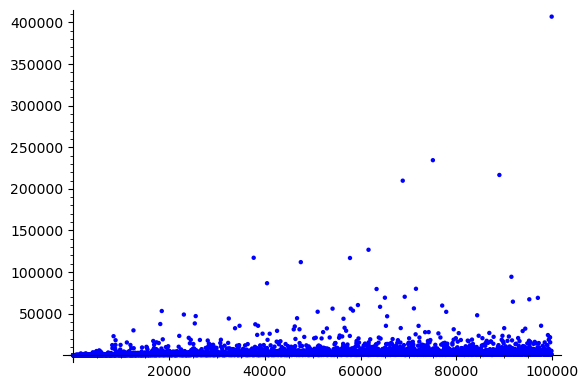
\includegraphics[width=12cm]{MCount.png}
%  \label{fig:boat1}
%  \caption{Číslo $d(\mathbb{F}_p)$}
%\end{center}
%\end{figure}
%\end{center}
\begin{figure}[h]
\centering
\begin{minipage}{.5\textwidth}
  \centering
  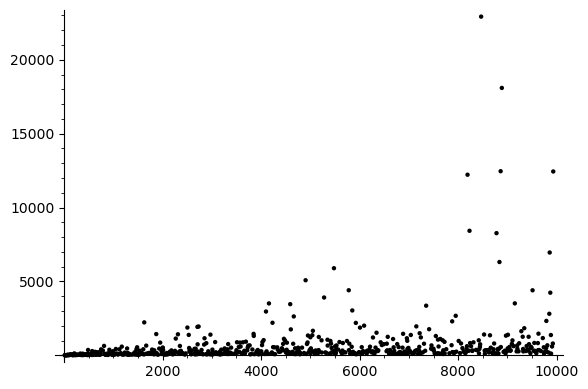
\includegraphics[width=.9\linewidth]{MCount1.png}
  \captionof{figure}{Číslo $d(\mathbb{F}_p)$ pro $p < 10^4$}
  \label{LOL}
\end{minipage}%
\begin{minipage}{.5\textwidth}
  \centering
  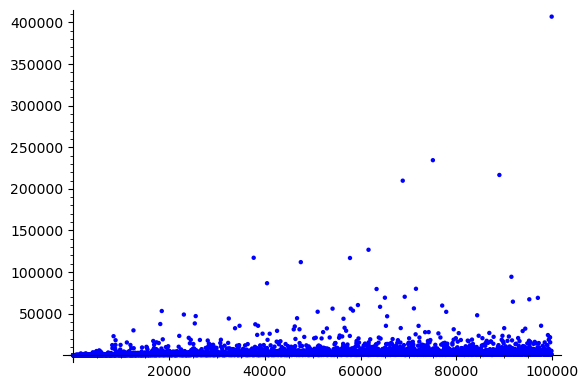
\includegraphics[width=.9\linewidth]{MCount.png}
  \captionof{figure}{Číslo $d(\mathbb{F}_p)$ pro $p < 10^5$}
  \label{XD}
\end{minipage}
\end{figure}

Některé hodnoty $d(\mathbb{F}_p)$ jsou mnohem vyšší než ostatní, například pro $p=99859$ máme $d(\mathbb{F}_p) = 406954$. I po sobě jdoucí prvočísla mohou mít disproporcionálně různé počty medúz. Na příklad pro prvočíslo $1619$ je počet medúz roven $d(\mathbb{F}_{1619}) = 56$ a hned o dům dál u prvočísla $1627$ nalezneme v grafu enormní počet $d(\mathbb{F}_{1627}) =2227$ medúz, skoro čtyřicetkrát více. Na grafu výše tak vidíme chování extrémních případů, žádné zjevné trendy se nevyskytují. 

Číslo $s(\mathbb{F}_p)$ se chová mnohem rozumněji. Případy, kdy $d(\mathbb{F}_p)$ je velké, jsou právě ty, kdy jsou hejna malá, a proto mezi hodnotami $s(\mathbb{F}_q)$ nenacházíme odlehlé hodnoty. Na obrázku \ref{fi} vidíme chování $s(\mathbb{F}_p)$ pro $p<10^5$.\\

\begin{figure}[h]
\centering
  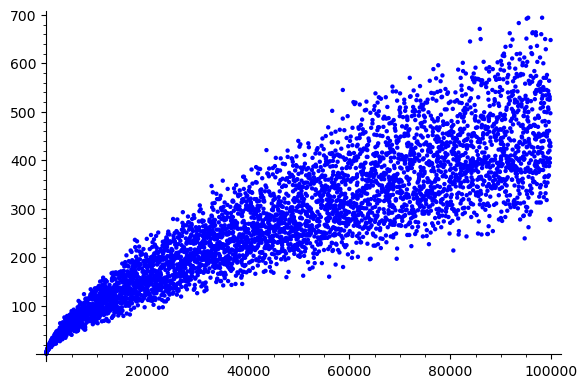
\includegraphics[width=9cm]{SCount.png}
  \caption{Číslo $s(\mathbb{F}_p)$ pro $p < 10^5$}
   \label{fi}
\end{figure}


Autoři článku \cite{Meduza} propojili $AG$ posloupnost s teorií eliptických křivek, těm se budeme věnovat v kapitole \ref{ctyri}. Pomocí této teorie dokázali netriviální dolní odhad na číslo $d(\mathbb{F}_q)$, resp. jejich postup ohraničí dokonce číslo $s(\mathbb{F}_q)$. Hlavním výsledkem jejich článku je tvrzení, že pro libovolně malé $\varepsilon > 0$ a $q$ dostatečně velké platí:
$$s(\mathbb{F}_q) \geqslant \left( \frac{1}{2} - \varepsilon \right) \sqrt{q}.$$
V závěru práce spekulují, zda je tento odhad asymptoticky optimální a navrhují odhad $d(\mathbb{F}_q) \geqslant O(\sqrt{q} \log \log q)$. Tento odhad není nijak podložen. Pojďme se těmto odhadům věnovat.

Nejprve, jak optimální opravdu je odhad $s(\mathbb{F}_q)$ (resp. $d(\mathbb{F}_q)$)?  Porovnejme číslo $s(\mathbb{F}_q)$ s~funkcí $\sqrt{q}$:

\begin{figure}[h]
\centering
  \includegraphics[width=11cm]{SCountLOL.png}
  \label{fig:boat2}
\caption{Porovnání $s(\mathbb{F}_p)$ s funkcemi $\sqrt{p}$, $\sqrt{p} \log \log p$ a $\frac{1}{4} \sqrt{p} \log \log p$.}
\end{figure}

Těsnější odhad získáme, pokud uvážíme funkce $f \in O(\sqrt{q} \log \log q)$, podle návrhu v~\cite{Meduza}. I když se autoři horním odhadům na číslo $s(\mathbb{F}_q)$ nevěnovali, zdánlivě jej můžeme též odhadnout funkcí tvaru $c \sqrt{q} \log \log q$.
\begin{domnenka}\label{dd}
Existuje $c \in \mathbb{R}^{+}$ takové, že pro dostatečně velké $q$ platí:
$$c \sqrt{q} \log \log q \geqslant s(\mathbb{F}_q) \geqslant \frac{1}{4} \sqrt{q} \log \log q.$$
\end{domnenka}

Spočítali jsme hodnoty $d(\mathbb{F}_q)$ a $s(\mathbb{F}_q)$ pro vybrané hodnoty $p < 10^6$. Pro tato prvočísla platí $s(\mathbb{F}_p) > \frac{1}{4} \sqrt{p} \log \log p$, pro $p=350431$ platí $s(\mathbb{F}_p) = 1571 > \sqrt{p} \log \log p \approx 1507.6$.

Další otázkou může být, jak spolu souvisí čísla $d(\mathbb{F}_q)$ a $s(\mathbb{F}_q)$. Zjevně platí nerovnost $s(\mathbb{F}_q) \geqslant d(\mathbb{F}_q)$. Co lepšího můžeme říci? Pokud se podíváme, jak se plošně chová číslo $\frac{s(\mathbb{F}_q)}{d(\mathbb{F}_q)}$ získáme velmi zajímavý graf, viz obrázek \ref{figg}. Vidíme, že pro $p>7$ se číslo $\frac{s(\mathbb{F}_q)}{d(\mathbb{F}_q)}$ drží pod hodnotou $0.75$ (maximální podíl nastane pro $p=47$). To naznačuje, že libovolný horní odhad na číslo $s(\mathbb{F}_q)$ nemůže mít jako důsledek asymptoticky silnější odhad na číslo $d(\mathbb{F}_q)$.  



\begin{figure}[h]
\centering
  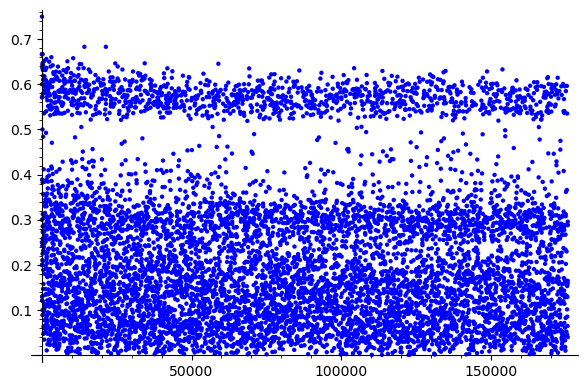
\includegraphics[width=8cm]{Podil.png}

  \caption{Hodnoty $s(\mathbb{F}_p)/d(\mathbb{F}_p)$ pro $p < 1.2 \cdot 10^5$}
  \label{figg}
\end{figure}





\section{HG posloupnost}


V první kapitole jsme si ukázali, že pokud místo aritmetického a geometrického průměru zvolíme jinou dvojici průměrů, získáme posloupnosti úzce propojené s $AG$ posloupností. Co tedy se podívat na jejich obdoby v konečných tělesech? Nejprve zapojme do práce geometrický a harmonický průměr, kde definujeme harmonický průměr dvou nenulových čísel s nenulovým součtem jako:
$$\frac{2}{\frac{1}{a}+\frac{1}{b}} = \frac{2ab}{a+b},$$
kde $\frac{1}{a}$ je multiplikativní inverze čísla $a$. Definujme pak $HG$-posloupnost nad konečným tělesem.


\begin{definice}
Ať $a,b$ jsou různé prvky $\mathbb{F}_q ^{\times}$ splňují $\phi_q (ab) = 1$. Pak definujeme $HG_{\mathbb{F}_q}(a,b)$ jako posloupnost $((a_n,b_n))_{n=0}^{\infty}$ s $(a_0,b_0) = (a,b)$ a:
\begin{equation*}
\left(a_{n+1},b_{n+1} \right) = \left(\frac{2}{\frac{1}{a_n} + \frac{1}{b_n}}, \sqrt{a_n b_n} \right),
\end{equation*}
přičemž $b_{n+1}$ volíme tak, že $\phi_q (a_{n+1} b_{n+1}) = 1$.
\end{definice}

\begin{definice}
Definujme \textit{roj} $\HG_{\mathbb{F}_q} = (V,E)$ jako orientovaný graf, kde $(a,b) \in V$, právě pokud platí $\phi_q(ab) = 1$, a $\big((a,b),(c,d)\big) \in E$, právě pokud platí $(c,d) = (a_1,b_1)$, kde $(a_0,b_0) = (a,b)$.
\end{definice}

\begin{priklad}\label{pr8}
Podívejme se na roje $HG_{\mathbb{F}_p}$ pro $p=7$ a $11$. Pro $p=7$ je jediná komponenta medúza, jejíž cyklus je následující:
$$
(2,1) \mapsto (6,3) \mapsto (4,2) \mapsto (5,6) \mapsto (1,4) \mapsto (3,5) \mapsto (2,1),
$$

V roji $\HG_{\mathbb{F}_{11}}$ zvolme dvojice $(3,1)$ a $(5,1)$ a pišme jejich posloupnosti:
\begin{align*}
(3,1) \mapsto (7,6) \mapsto (9,3) \mapsto (10,7) \mapsto (5,9) &\mapsto (8,10) \mapsto (4,5) \mapsto (2,8) \mapsto (1,4) \mapsto (6,2) \mapsto (3,1),\\
(5,1) \mapsto (9,4) \mapsto (3,5) &\mapsto (1,9) \mapsto (4,3) \mapsto (5,1),\\
(6,10) \mapsto (2,7) \mapsto (8,6) &\mapsto (10,2) \mapsto (7,8) \mapsto (6,10).
\end{align*}


Tyto tři cykly jsou cykly všech medúz v $\HG_{\mathbb{F}_q}$. Druhé dvě z těchto medúz jsou přátelé, stejně jako v případě roje $\AG_{\mathbb{F}_{11}}$. 
\end{priklad}


Z příkladu \ref{pr8} se můžeme dovtípit, že tato posloupnost je pouze přestrojená AG posloupnost. V tomto přesvědčení nás může utvrdit počet hran a vrcholů i kritérium, kdy vrchol má předchůdce.

\begin{veta}
Graf $\HG_{\mathbb{F}_q}$ čítá $(q-1)(q-3)/2$ vrcholů a stejný počet hran.
\end{veta}
\textit{Důkaz.} Analogický k důkazu věty \ref{pocetprvkuAG}. \hfill $\square$


\begin{lemma}\label{q}
Vrchol $(a,b) \in \HG_{\mathbb{F}_q}$ má předchůdce, právě pokud platí $\phi_q(b^2-a^2)=1$.
\end{lemma}

\noindent \textit{Důkaz.} Nejprve předpokládejme $(a,b)$ má předchůdce $(c,d)$, platí tedy:
\begin{equation*}
a = \frac{2cd}{c+d}, \quad b = \sqrt{cd}.
\end{equation*}
Potom:
\begin{equation*}
b^2-a^2 = cd- \left(\frac{2 cd}{c+d} \right)^2 = cd \left( \frac{c-d}{c+d} \right)^2
\end{equation*}
je čtverec, protože pracujeme pouze s dvojicemi, jejichž součin je čtvercem. Naopak ať $b^2-a^2$ je čtverec a $x$ je nějaká jeho odmocnina. Pak uvažme vrchol $\Big(\frac{b^2+b  x}{a},\frac{b^2-bx}{a} \Big)$, jeho následník je: $$\left(\frac{2 b^2 (b+x)(b-x)}{a^2 \left(\frac{b^2+bx}{a} + \frac{b^2-bx}{a} \right)}, \sqrt{\frac{b^2(b^2-x^2)}{a^2}} \right)= \left(\frac{2 b^2 \cdot a^2}{2 a \cdot b^2 }, b \right) = \left(a, b \right).$$
 \hfill $\square$


\begin{dusledek}
Graf $\HG_{\mathbb{F}_q}$ je tvořen z několika medúz.
\end{dusledek}
\noindent \textit{Důkaz}. Analogický k důkazu věty \ref{meduzy}. \hfill $\square$\\

Rozdíl mezi oběma grafy je ten, že vrchol $(a,b)$ pro $a,b$ je součástí cyklu v \textit{právě jednom} z grafů $\AG_{\mathbb{F}_q}$ a $\HG_{\mathbb{F}_q}$ díky lemmatům \ref{p} a \ref{q}. To a nebo věta \ref{agh} nám napovídají, jaké bude konkrétní propojení těchto dvou grafů.

\begin{veta}
Platí isomorfismus grafů $\AG_{\mathbb{F}_q} \cong \HG_{\mathbb{F}_q}$.
\end{veta}
\noindent \textit{Důkaz.} Uvažme zobrazení $\psi : \AG_{\mathbb{F}_q} \longrightarrow \HG_{\mathbb{F}_q}$ určené předpisem $\psi((a,b)) = (1/a,1/b)$. Ukážeme, že toto zobrazení definuje mezi grafy isomorfismus. Opravdu, uvažme orientovanou hranu v grafu $\AG_{\mathbb{F}_q}$: 
$$(a,b) \longmapsto \left(\frac{a+b}{2}, \sqrt{ab} \right),$$
poté v grafu $\HG_{\mathbb{F}_q}$ má $\psi((a,b))$ hranu:
$$\psi ((a,b)) = \left(\frac{1}{a}, \frac{1}{b} \right) \longmapsto \left(\frac{2/ab}{1/a+1/b}, \sqrt{\frac{1}{ab}} \right) = \left( \frac{2}{a+b}, \frac{1}{\sqrt{ab}} \right) = \psi \left( \left( \frac{a+b}{2}, \sqrt{ab} \right) \right).$$
Jelikož $\psi$ se zjevně bijekce mezi $\AG_{\mathbb{F}_q}$ a $\HG_{\mathbb{F}_q}$, definuje mezi grafy isomorfismus.\hfill $\square$\\


\chapter{AH posloupnost}\label{AH}
Zatím jsme pracovali s dvěma dvojicemi průměrů z trojice -- aritmetický, geometrický a~harmonický. V této kapitole se proto podíváme i na tu poslední -- aritmetický a harmonický průměr. K této ani $HG$ posloupnosti nad konečnými tělesy neexistuje podle nejlepšího svědomí autora žádná literatura. Strávíme nějaký čas nad tvary grafů - případ $AH$ posloupnosti je totiž na dvakrát tolik zajímavý, jako ty předchozí.

\section{Základní poznatky}

Tentokrát již ze začátku nebudeme pracovat pouze nad konečným tělesem, ale i s bodem v~nekonečnu.

\begin{definice}
Ať $K$ je těleso. Pak definujeme \textit{projektivní přímku} $\mathbb{P}^{1} (K)$ jako množinu tříd nenulových vektorů $(a_1:a_2) \in K^2$ s relací ekvivalence $(a:b) \sim (c:d)$, právě pokud existuje $\lambda \in K$ splňující $(a,b) = \lambda (c,d)$.
\end{definice}
Pro třídu $(a:b)$ pro $b \neq 0$ zvolíme reprezentanta $\left(\frac{a}{b} : 0 \right)$ a identifikujeme třídu $(a:b)$ s číslem $\frac{a}{b} \in \mathbb{F}_q$. Jediná třída, která takto není pokryta, je třída $(1:0)$, tu ztotožníme s~\textit{bodem v nekonečnu} $\infty$. 
Ten pro $m \in \mathbb{F}_q$ splňuje:
\begin{enumerate}
\item $\frac{1}{0} = \infty$ a $\frac{1}{\infty} = 0$,
\item $\infty+m = \infty$,
\item $\infty \cdot m = \infty$ pro $m \neq 0$,
\item $\infty \times \infty = \infty$.
\end{enumerate}


Pomocí projektivní přímky můžeme v plném rozsahu definovat a studovat $AH$ posloupnost nad konečným tělesem.

\begin{definice}
Ať $a,b \in \mathbb{F}_q ^{\times}$ jsou různé. Pak definujeme $\AH_{\mathbb{F}_q}(a,b)$ jako posloupnost $((a_n,b_n))_{n=0}^{\infty}$ s $(a_0,b_0) = (a,b)$ a:
\begin{equation*}
\left(a_{n+1},b_{n+1} \right) = \left(\frac{a_n+b_n}{2}, \frac{2}{\frac{1}{a_n} + \frac{1}{b_n}} \right).
\end{equation*}
\end{definice}

Všimněme si, že následník bodu $(a,-a)$ pro $a \in \mathbb{F}_q$ je $(0,\infty)$ a následník $(0,\infty)$ je $(\infty,0)$. Bod $(\infty,0)$ je následník sama sebe. 

Pokud $\phi_q(2) \neq 1$, tak se každý \textit{afinní}\footnote[3]{Bod $(a,b) \in \AH_{\mathbb{F}_q}$ takový, že $a,b \in \mathbb{F}_q$, nazveme afinním.} bod zobrazí opět na afinní bod. Připusťme, že pro nějaká $(a_0,b_0)$ a $n$ nezáporné platí $1/a_{n+1} + 1/b_{n+1} = 0$, pak i $a_{n+1} + b_{n+1} = 0$. Musí pak být:
\begin{align*}
\frac{a_n+b_n}{2} + \frac{2 a_n b_n}{a_n + b_n} &= 0,\\
(a_n+b_n)^2 + 4 a_n b_n &= 0,\\
\left(\frac{a_n}{b_n} + 1 \right)^2 + \frac{4a_n}{b_n} &= 0,\\
\left(\frac{a_n}{b_n}\right)^2 + \frac{6a_n}{b_n} + 1 &= 0.
\end{align*}
Poznamenejme, že $b_n \neq 0$. Tato kvadratická rovnice má kořen nad $\mathbb{F}_q$, právě pokud $2$ je v~$\mathbb{F}_q$ čtvercem. Pro tělesa, kde $2$ je čtvercem, mohou některé posloupnosti $\AH_{\mathbb{F}_q}(a,b)$ obsahovat body v nekonečny a~musíme již pracovat s projektivní přímkou. Budeme vždy pracovat pouze s posloupnostmi, které obsahují alespoň jeden afinní prvek. Nejprve podíváme na tělesa $\mathbb{F}_q$ s $q \equiv \pm 3 \pmod{8}$.

\begin{definice}
Definujme \textit{roj} $\AH_{\mathbb{F}_q} = (V,E)$ jako orientovaný graf, kde $(a,b) \in V$ pokud $a,b \in \mathbb{F}_q$, nebo $\lbrace a,b \rbrace = \lbrace 0,\infty \rbrace$. Pro libovolná $a,b,c,d \in \mathbb{P}^1 (\mathbb{F}_q)$ platí $\Big((a,b), (c,d) \Big) \in E$, právě pokud $(c,d) = (a_1,b_1)$, kde $(a_0,b_0) = (a,b)$. 
\end{definice}

\begin{umluva}
Každý afinní bod má v grafu zjevně nejvýše dva předchůdce. Toto je zdárně porušeno pro body v nekonečnu, kde bod $(0,\infty)$ má předchůdců hned $q-1$ -- body $(a,-a)$, viz příklad \ref{pr4}. Čistě z důvodu elegance, která se prokáže v kapitole \ref{5}, budeme uvažovat $\frac{q-1}{2}$ bodů $(0,\infty)$ a $(\infty,0)$, každý příslušící jedné dvojici bodů $(a,-a)$ a~$(-a,a)$. Domluvíme se tedy, že pro $a,b \in \mathbb{F}_q ^{\times}$ splňující $a \neq \pm b$ body $(a,-a)$ a~$(b,-b)$ neleží ve stejné komponentě souvislosti grafu $\AH_{\mathbb{F}_q}$. Naopak uvažujme, že body $(a,-a)$ a $(-a,a)$ ve stejné komponentě souvislosti leží.
\end{umluva}

\begin{priklad}\label{pr4}
Podívejme se na graf $\AH_{\mathbb{F}_{11}}$ a dva prvky, $(1,3)$ a $(3,2)$. Komponenta souvislosti obsahující $(1,3)$ je medúza, komponenta obsahující $(3,2)$ je tvořena z cyklu, ke každému prvku cyklu je připojen vyvážený binární strom hloubky $2$. 

 
\begin{figure}[!h]
\begin{minipage}{0.5\textwidth}
\centering
 \begin{tikzpicture}[node distance=2cm]
\def\s{0.7}
\def\l{2mm}
\def\w{1mm}
\def\t{3pt}
%\draw[line width=.5pt,black,fill=yellow] (0:4cm) circle (3pt);

%\draw[line width=.5pt,black,fill=yellow] (60:4cm) circle (3pt);
%\draw[line width=.5pt,black,fill=yellow] (120:4cm) circle (3pt);
%\draw[line width=.5pt,black,fill=yellow] (180:4cm) circle (3pt);
%\draw[line width=.5pt,black,fill=yellow] (240:4cm) circle (3pt);
%\draw[line width=.5pt,black,fill=yellow] (300:4cm) circle (3pt);
%\draw[line width=.5pt,black,fill=yellow] (0:8cm) circle (3pt);
 
%\draw[line width=.5pt,black,fill=yellow] (60:8cm) circle (3pt);
%\draw[line width=.5pt,black,fill=yellow] (120:8cm) circle (3pt);
%\draw[line width=.5pt,black,fill=yellow] (180:8cm) circle (3pt);
%\draw[line width=.5pt,black,fill=yellow] (240:8cm) circle (3pt);
%\draw[line width=.5pt,black,fill=yellow] (300:8cm) circle (3pt);

\node [draw,black,fill=yellow, circle,inner sep=\t, scale=\s, name=c1]      at (180:1cm) {$3,2$};
\node [draw,black,fill=yellow, circle,inner sep=\t, scale=\s, name=c2]      at (0:1cm) {$8,9$};
\node [draw,black,fill=yellow, circle,inner sep=\t, scale=\s, name=b2]      at (0:2cm) {$2,3$};
\node [draw,black,fill=yellow, circle,inner sep=\t, scale=\s, name=b1]      at (180:3cm) {$9,8$};
\node [draw,black,fill=yellow, circle,inner sep=\t, scale=\s, name=d1]      at (160:5cm) {$6,1$};
\node [draw,black,fill=yellow, circle,inner sep=\t, scale=\s, name=d2]      at (200:5cm) {$1,6$};
\node [draw,black,fill=yellow, circle,inner sep=\t, scale=\s, name=d3]      at (20:4cm) {$5,10$};
\node [draw,black,fill=yellow, circle,inner sep=\t, scale=\s, name=d4]      at (340:4cm) {$10,5$};
\draw [-{Stealth[length=\l, width=\w]}](c1) to [out=45,in=135](c2);
\draw [-{Stealth[length=\l, width=\w]}](c2) to [out=225,in=315](c1);
\draw [-{Stealth[length=\l, width=\w]}](b1) to (c1);
\draw [-{Stealth[length=\l, width=\w]}](b2) to (c2);
\draw [-{Stealth[length=\l, width=\w]}](d1) to (b1);
\draw [-{Stealth[length=\l, width=\w]}](d2) to (b1);
\draw [-{Stealth[length=\l, width=\w]}](d3) to (b2);
\draw [-{Stealth[length=\l, width=\w]}](d4) to (b2);
%\node[text width=3cm] at (300:4cm) {$(1,2)$};
%\node[text width=3cm] at (0:4cm) {$(5,3)$};
\end{tikzpicture}


\end{minipage}
\begin{minipage}{0.2\textwidth}

\begin{flushright}
 \begin{tikzpicture}[node distance=2cm]
\def\s{0.7}
\def\l{2mm}
\def\w{1mm}
\def\t{3pt}


\node [draw,black,fill=yellow, circle,inner sep=\t, scale=\s, name=a1]      at (90:2cm) {$1,3$};
\node [draw,black,fill=yellow, circle,inner sep=\t, scale=\s, name=a2]      at (0:2cm) {$2,7$};
\node [draw,black,fill=yellow, circle,inner sep=\t, scale=\s, name=a3]      at (270:2cm) {$10,8$};
\node [draw,black,fill=yellow, circle,inner sep=\t, scale=\s, name=a4]      at (180:2cm) {$9,4$};
\node [draw,black,fill=yellow, circle,inner sep=\t, scale=\s, name=b1]      at (90:4cm) {$4,9$};
\node [draw,black,fill=yellow, circle,inner sep=\t, scale=\s, name=b2]      at (0:4cm) {$3,1$};
\node [draw,black,fill=yellow, circle,inner sep=\t, scale=\s, name=b3]      at (270:4cm) {$7,2$};
\node [draw,black,fill=yellow, circle,inner sep=\t, scale=\s, name=b4]      at (180:3.5cm) {$8,10$};
\draw [-{Stealth[length=\l, width=\w]}](a1) to (a2);
\draw [-{Stealth[length=\l, width=\w]}](a2) to (a3);
\draw [-{Stealth[length=\l, width=\w]}](a3) to (a4);
\draw [-{Stealth[length=\l, width=\w]}](a4) to (a1);
\draw [-{Stealth[length=\l, width=\w]}](b1) to (a1);
\draw [-{Stealth[length=\l, width=\w]}](b2) to (a2);
\draw [-{Stealth[length=\l, width=\w]}](b3) to (a3);
\draw [-{Stealth[length=\l, width=\w]}](b4) to (a4);
%\node[text width=3cm] at (300:4cm) {$(1,2)$};
%\node[text width=3cm] at (0:4cm) {$(5,3)$};
\end{tikzpicture}
\end{flushright}

\end{minipage}

\caption{Komponenty souvislosti grafu $\AH_{\mathbb{F}_{11}}$.}
\end{figure} 
 
 
Dále se podívejme na graf $\AH_{\mathbb{F}_{23}}$. Zde pro nás jsou zajímavé dvě komponenty souvislosti, konkrétně ty obsahující body $(1,5)$ a $(1,-1) \in \AH_{\mathbb{F}_q}$. Ty vypadají následovně.

\begin{figure}[!h]
\begin{center}
\begin{tikzpicture}[node distance=2cm]
\def\s{0.7}
\def\l{2mm}
\def\w{1mm}
\def\t{3pt}
%\draw[line width=.5pt,black,fill=yellow] (0:4cm) circle (3pt);

%\draw[line width=.5pt,black,fill=yellow] (60:4cm) circle (3pt);
%\draw[line width=.5pt,black,fill=yellow] (120:4cm) circle (3pt);
%\draw[line width=.5pt,black,fill=yellow] (180:4cm) circle (3pt);
%\draw[line width=.5pt,black,fill=yellow] (240:4cm) circle (3pt);
%\draw[line width=.5pt,black,fill=yellow] (300:4cm) circle (3pt);
%\draw[line width=.5pt,black,fill=yellow] (0:8cm) circle (3pt);
 
%\draw[line width=.5pt,black,fill=yellow] (60:8cm) circle (3pt);
%\draw[line width=.5pt,black,fill=yellow] (120:8cm) circle (3pt);
%\draw[line width=.5pt,black,fill=yellow] (180:8cm) circle (3pt);
%\draw[line width=.5pt,black,fill=yellow] (240:8cm) circle (3pt);
%\draw[line width=.5pt,black,fill=yellow] (300:8cm) circle (3pt);

\node [draw,black,fill=yellow, circle,inner sep=\t, scale=\s, name=c1]      at (180:1cm) {};
\node [draw,black,fill=yellow, circle,inner sep=\t, scale=\s, name=c2]      at (0:1cm) {};
\node [draw,black,fill=yellow, circle,inner sep=\t, scale=\s, name=b2]      at (0:3cm) {};
\node [draw,black,fill=yellow, circle,inner sep=\t, scale=\s, name=b1]      at (180:3cm) {};
\node [draw,black,fill=yellow, circle,inner sep=\t, scale=\s, name=d1]      at (160:5cm) {};
\node [draw,black,fill=yellow, circle,inner sep=\t, scale=\s, name=d2]      at (200:5cm) {};
\node [draw,black,fill=yellow, circle,inner sep=\t, scale=\s, name=d3]      at (20:5cm) {};
\node [draw,black,fill=yellow, circle,inner sep=\t, scale=\s, name=d4]      at (340:5cm) {};
\node [draw,black,fill=yellow, circle,inner sep=\t, scale=\s, name=e1]      at (170:7cm) {};
\node [draw,black,fill=yellow, circle,inner sep=\t, scale=\s, name=e2]      at (190:7cm) {};
\node [draw,black,fill=yellow, circle,inner sep=\t, scale=\s, name=e3]      at (210:7cm) {};
\node [draw,black,fill=yellow, circle,inner sep=\t, scale=\s, name=e4]      at (150:7cm) {};
\node [draw,black,fill=yellow, circle,inner sep=\t, scale=\s, name=f1]      at (10:7cm) {};
\node [draw,black,fill=yellow, circle,inner sep=\t, scale=\s, name=f2]      at (30:7cm) {};
\node [draw,black,fill=yellow, circle,inner sep=\t, scale=\s, name=f3]      at (330:7cm) {};
\node [draw,black,fill=yellow, circle,inner sep=\t, scale=\s, name=f4]      at (350:7cm) {};
\draw [-{Stealth[length=\l, width=\w]}](c1) to [out=45,in=135](c2);
\draw [-{Stealth[length=\l, width=\w]}](c2) to [out=225,in=315](c1);
\draw [-{Stealth[length=\l, width=\w]}](b1) to (c1);
\draw [-{Stealth[length=\l, width=\w]}](b2) to (c2);
\draw [-{Stealth[length=\l, width=\w]}](d1) to (b1);
\draw [-{Stealth[length=\l, width=\w]}](d2) to (b1);
\draw [-{Stealth[length=\l, width=\w]}](d3) to (b2);
\draw [-{Stealth[length=\l, width=\w]}](d4) to (b2);
\draw [-{Stealth[length=\l, width=\w]}](e1) to (d1);
\draw [-{Stealth[length=\l, width=\w]}](e4) to (d1);
\draw [-{Stealth[length=\l, width=\w]}](e2) to (d2);
\draw [-{Stealth[length=\l, width=\w]}](e3) to (d2);
\draw [-{Stealth[length=\l, width=\w]}](f1) to (d3);
\draw [-{Stealth[length=\l, width=\w]}](f2) to (d3);
\draw [-{Stealth[length=\l, width=\w]}](f3) to (d4);
\draw [-{Stealth[length=\l, width=\w]}](f4) to (d4);
%\node[text width=3cm] at (300:4cm) {$(1,2)$};
%\node[text width=3cm] at (0:4cm) {$(5,3)$};
\end{tikzpicture}
\end{center}
\caption{Komponenta roje $\AH_{\mathbb{F}_{23}}$ obsahující $(1,5)$.}
\label{bigboy}
\end{figure}

\begin{figure}[!h]
\begin{center}
\begin{tikzpicture}[node distance=2cm]
\def\s{1.05}
\def\l{2mm}
\def\w{1mm}
\def\t{3pt}
%\draw[line width=.5pt,black,fill=yellow] (0:4cm) circle (3pt);

%\draw[line width=.5pt,black,fill=yellow] (60:4cm) circle (3pt);
%\draw[line width=.5pt,black,fill=yellow] (120:4cm) circle (3pt);
%\draw[line width=.5pt,black,fill=yellow] (180:4cm) circle (3pt);
%\draw[line width=.5pt,black,fill=yellow] (240:4cm) circle (3pt);
%\draw[line width=.5pt,black,fill=yellow] (300:4cm) circle (3pt);
%\draw[line width=.5pt,black,fill=yellow] (0:8cm) circle (3pt);
 
%\draw[line width=.5pt,black,fill=yellow] (60:8cm) circle (3pt);
%\draw[line width=.5pt,black,fill=yellow] (120:8cm) circle (3pt);
%\draw[line width=.5pt,black,fill=yellow] (180:8cm) circle (3pt);
%\draw[line width=.5pt,black,fill=yellow] (240:8cm) circle (3pt);
%\draw[line width=.5pt,black,fill=yellow] (300:8cm) circle (3pt);

\node [draw,black,fill=yellow, circle,inner sep=\t, scale=2*\s/3, name=a1]      at (0,0) {$0,\infty$};
\node [draw,black,fill=yellow, circle,inner sep=\t, scale=2*\s/3, name=a2]      at (90:3cm) {$\infty,0$};
\node [draw,black,fill=yellow, circle,inner sep=\t, scale=2*\s/3, name=b1]      at (0:3cm) {$1,-1$};
\node [draw,black,fill=yellow, circle,inner sep=\t, scale=2*\s/3, name=b2]      at (180:3cm) {$-1,1$};
\node [draw,black,fill=yellow, circle,inner sep=\t, scale=2*\s/3, name=d1]      at (160:6cm) {$17,4$};
\node [draw,black,fill=yellow, circle,inner sep=\t, scale=2*\s/3, name=d2]      at (200:6cm) {$4,17$};
\node [draw,black,fill=yellow, circle,inner sep=\t, scale=2*\s/3, name=d3]      at (20:6cm) {$19,6$};
\node [draw,black,fill=yellow, circle,inner sep=\t, scale=2*\s/3, name=d4]      at (340:6cm) {$6,19$};
\draw [-{Stealth[length=\l, width=\w]}](a2) to [out=135,in=45,looseness=8](a2);
\draw [-{Stealth[length=\l, width=\w]}](b1) to (a1);
\draw [-{Stealth[length=\l, width=\w]}](b2) to (a1);
\draw [-{Stealth[length=\l, width=\w]}](a1) to (a2);
\draw [-{Stealth[length=\l, width=\w]}](d1) to (b2);
\draw [-{Stealth[length=\l, width=\w]}](d2) to (b2);
\draw [-{Stealth[length=\l, width=\w]}](d3) to (b1);
\draw [-{Stealth[length=\l, width=\w]}](d4) to (b1);
%\node[text width=3cm] at (300:4cm) {$(1,2)$};
%\node[text width=3cm] at (0:4cm) {$(5,3)$};
\end{tikzpicture}
\end{center}
\caption{Komponenta roje $\AH_{\mathbb{F}_{23}}$ obsahující $(1,-1)$.}
\label{bugboy}
\end{figure}
\end{priklad}

Na příkladu \ref{pr4} vidíme, že pro $q \equiv \pm 3 \pmod{8}$ při vizualizaci $\AH$ posloupnosti získáme krom medúz i tzv. \textit{vulkány hloubky $2$}. V případě $q \equiv \pm 1 \pmod{8}$ jsou tyto vulkány dokonce ještě hlubší a některé obsahují $(\infty,0)$. Tato terminologie není vybraná autorem, setkáme se s ní v kontextu eliptických křivek \cite{Suchanek}. 
\begin{definice}
Souvislý orientovaný graf $V$ nazveme \textit{vulkánem hloubky $k$}, pokud lze jeho vrcholy rozdělit do $k+1$ disjunktních množin $V_0,\dots,V_k$ a:
\begin{enumerate}
\item Podgraf grafu $V$ obsahující $V_0$ je cyklus, kde každý jeho člen má unikátního předchůdce mimo cyklus,
\item pro $0 <i < k$ má každý vrchol $W \in V_i$ unikátního následníka ve $V_{i-1}$ a dva předchůdce ve $V_{i+1}$,
\item každý prvek $V_k$ je listem.
\end{enumerate}
\end{definice}
Všimněme si, že medúza je pouze vulkánem hloubky $1$. Předtím, než ukážeme, že grafy $AH$ posloupnosti pro $q = \pm 3 \pmod{8}$ nabývají těchto tvarů, se pozastavme nad spojením $AH$ posloupnosti s dvěma předchozími posloupnostmi, které jsme studovali. I když větší vulkány $AG$ posloupnost nikdy netvoří, pro například $p \equiv -1 \pmod{4}$ získáme v~některých případech $AH$ posloupnosti též medúzy. Klíčové rozdělení bude podle $\phi(ab)$ pro jednotlivé dvojice. Hned uvidíme, že toto číslo je pro jednotlivé komponenty souvislosti stejné a~dokážeme silnější tvrzení. 
\begin{veta}\label{pocetv}
Buď $q = p^k$ mocnina prvočísla. Pak:
\begin{enumerate}
\item počet afinních vrcholů $(a,b) \in \AH_{\mathbb{F}_q}$ takových, že $\phi_q(ab) = 1$, je $(q-1)(q-3)/2$, 
\item počet afinních vrcholů $(a,b) \in \AH_{\mathbb{F}_q}$ takových, že $\phi_q(ab) = -1$, je $(q-1)^2/2$,
\item počet hran v celém grafu vycházejících z afinních vrcholů je $(q-1)(q-2)$.
\end{enumerate}

\end{veta}  
\noindent \textit{Důkaz.} V případě, kdy $ab$ je v $\mathbb{F}_q$ nenulovým čtvercem, leží v roji $\AH_{\mathbb{F}_q}$ právě dvojice $(a,b)$, až na případ, kdy $a=b$. Pokud je součin dvou prvků čtverec, tak jsou buď oba čtverce, nebo ani jeden. Počet dvojic nenulových prvků $(a,b)$, jejichž součin je čtverec, spočítáme tedy součtem počtů dvojic různých čtverců, resp. nečtverců. Toto je $(q-1)/2 \cdot (q-3)/2 + (q-1)/2 \cdot (q-3)/2 =  (q-1)(q-3)/2$.

V případě, kdy $ab$ není v $\mathbb{F}_q$ nenulovým čtvercem, leží v roji $\AH_{\mathbb{F}_q}$ všechny dvojice $(a,b)$. Takové dvojice mají jedno složku, která je čtvercem, a druhou, která není. Vyhovující počet je proto $(q-1)/2 \cdot (q-1)/2 + (q-1)/2 \cdot (q-1)/2 = (q-1)^2/2$. Konečně, z každého afinního vrcholu vychází právě jedna hrana, proto počet hran je:
$$\frac{(q-1)(q-3)}{2}+\frac{(q-1)^2}{2} = (q-1)(q-2).$$  \hfill $\square$\\



Grafy $\AH_{\mathbb{F}_q}$ a $\AG_{\mathbb{F}_q}$ jsou velmi odlišné. Na příkladu \ref{pr3} vidíme, že komponenty roje $AG_{\mathbb{F}_q}$ mohou mít mnohonásobně více prvků, než je $q$. Zato v případě $AH$ posloupnosti počet prvků značně omezí stejný invariant, jako v reálném případě - součin jednotlivých složek prvků. 

\begin{lemma}\label{fix}
Uvažme roj $\AH_{\mathbb{F}_q}$ a nějakou jeho komponentu souvislosti $V$. Pak je přes všechny afinní vrcholy $(a,b) \in V$ součin $ab$ invariantní.
\end{lemma}
\noindent \textit{Důkaz.} Stačí nám ukázat, že pro vrchol $(a,b)$ a jeho následníka platí $a_1 b_1 = ab$, jelikož $(a_1,b_1)$ má právě dva předchůdce, $(a,b)$ a $(b,a)$. A opravdu:
\begin{equation*}
a_1 b_1 = \frac{a+b}{2} \cdot \frac{2ab}{a+b} = ab.
\end{equation*} 
\hfill $\square$\\

\begin{dusledek}\label{fixab}
Každá komponenta souvislosti v roji $\AH_{\mathbb{F}_q}$ obsahuje nejvýše $q-1$ afinních vrcholů.
\end{dusledek}
\noindent \textit{Důkaz.} Pro dané nenulové $k \in \mathbb{F}_q$ je nad $\mathbb{F}_q$ jistě $q-1$ dvojic se součinem $k$, konkrétně $\left(a, \frac{k}{a}\right)$ pro $a \in \mathbb{F}_q ^{\times}$. Podle předchozího lemmatu \ref{fix} mají všechny prvky jedné souvislé komponenty stejný součin prvků, je jich proto nejvýše $q-1$. \hfill $\square$\\

Poznamenejme, že ze všech $q-1$ dvojic prvků s daným součinem ne nutně všechny leží v roji, například v tělese $\mathbb{F}_{11}$ pro součin roven čtyřem nevyhovuje dvojice $(2,2)$. Lemma, které jsme zmínili před chvílí, nám též umožní adaptovat větu \ref{isom}, tentokrát je totiž počet přátel grafů k dané souvislé komponentě velmi omezený.
\begin{definice}
Ať $(a,b) \in \AH_{\mathbb{F}_q}$ leží v souvislé komponentě $V$. Potom nazveme libovolnou souvislou komponentu obsahující prvek $(ka,kb)$ pro $k \in \mathbb{F}_q$ přítelem $V$.
\end{definice}

\begin{veta}\label{lol}
Ať $(a,b) \in \AH_{\mathbb{F}_q}$ leží v komponentě souvislosti $V$, která obsahuje pouze afinní vrcholy. Pak počet přátel $V$ je roven:
\begin{enumerate}
\item $q-1$, pokud $(-a,-b)$ neleží ve $V$,
\item $(q-1)/2$, pokud $(-a,-b)$ leží ve $V$.
\end{enumerate} 
\end{veta}
\noindent \textit{Důkaz.} Důkaz je prakticky stejný, jako důkaz věty \ref{isom}, tentokrát ale pokud pro $k \neq 1$ leží $(a,b)$ a $(ka,kb)$ ve stejné komponentě, podle lemmatu \ref{fix} musí platit $a b = k^2 ab$, tj. $k = - 1$. Nosná množina grupy $O_{k}$ sestrojené analogicky k důkazu věty \ref{isom} je proto podmnožinou $\lbrace 1,-1 \rbrace$ a dojdeme k tomu, že  $V$ má právě $\frac{q-1}{\ord_q (\pm 1)} \in  \left\lbrace q-1,\frac{q-1}{2}\right\rbrace$ přátel. \hfill $\square$\\

V případě, že komponenta obsahuje body v nekonečnu, pak předchůdci prvku $(0,\infty)$ jsou $(\pm a,\mp a)$, tedy tato komponenta má $(q-1)/2$ přátel. Poznamenejme, že ve zdánlivé většině grafů $\AH_{\mathbb{F}_q}$ se vyskytují komponenty s $q-1$ přáteli, stejně jako jiné komponenty, které mají přátel pouze $(q-1)/2$.

\begin{definice}
Ať $H \subseteq \AH_{\mathbb{F}_q}$ je komponenta souvislosti roje a $H_1,\dots,H_k$ jsou všichni její přátelé. Pak $H \cup H_1 \cup \dots \cup H_k$ nazvěme \textit{hejnem}.
\end{definice}
 

\section{Struktura grafů}

$AH$ posloupnost se od $AG$ posloupnosti na několika místech principiálně liší, přesto se na jednom místě shodují. Jejich grafy mají pozoruhodně pravidelnou strukturu. V pozdějších částech práce tuto strukturu do jisté míry vysvětlíme. Bez dalšího otálení proto pojďme opravdu dokázat, že grafy $\AH_{\mathbb{F}_q}$ mají tu strukturu, kterou jim připisujeme. Nejprve klasifikujeme, kdy má prvek předchůdce.

\begin{lemma}\label{lema}
Afinní vrchol $(a,b) \in \AH_{\mathbb{F}_q}$ má předchůdce, právě pokud $\phi_q(a^2-ab)=1$.
\end{lemma}

\noindent \textit{Důkaz.} Nejprve předpokládejme, že $(a,b)$ má předchůdce $(c,d)$, platí tedy:
\begin{equation*}
a = \frac{c+d}{2}, \quad b = \frac{2cd}{c+d}.
\end{equation*}
Potom:
\begin{equation*}
a(a-b) = \frac{c+d}{2} \left( \frac{c+d}{2} - \frac{2cd}{c+d} \right) =\left( \frac{c-d}{2}\right)^2
\end{equation*}
je čtverec. Naopak ať $a(a-b)$ je čtverec a $x$ je nějaká jeho odmocnina. Podle definice roje nemůže platit $a^2 \neq a(a-b)$, tedy v $\AH_{\mathbb{F}_q}$ leží vrchol $(a-x,a+x)$.  Jeho následník je: $$\left(\frac{a-x+a+x}{2}, \frac{2 (a-x)(a+x)}{a-x+a+x} \right)= \left(a, b \right).$$ \hfill $\square$\\

\begin{poznamka}
Lemma \ref{lema} pro $a=-b$ nám říká, že vrchol $(a,-a) \in \AH_{\mathbb{F}_q}$ má předchůdce, právě pokud platí $\phi_q(2) = 1$. 
\end{poznamka}

Díky tomuto tvrzení dokážeme poskytnout parciální odpověď na otázku, jak vypadají komponenty souvislosti v $\AH_{\mathbb{F}_q}$. Prozatím se zaměříme na případy $q \equiv 3,5 \pmod{8}$, lemma \ref{lema} nám rozdělí práci pro tyto dva případy.

\begin{dusledek}\label{dusl}
Uvažme afinní vrchol $(a,b) \in \AH_{\mathbb{F}_q}$. Potom:
\begin{enumerate}
\item pokud $\phi_q(-ab) = -1$, tak má právě jeden z vrcholů $(a,b)$ a $(b,a)$ v $\AH_{\mathbb{F}_q}$ předchůdce,
\item pokud $\phi_q(-ab) = 1$, tak mají v $\AH_{\mathbb{F}_q}$ předchůdce buď oba vrcholy $(a,b)$ a $(b,a)$, nebo ani jeden.
\end{enumerate}
\end{dusledek}
\noindent \textit{Důkaz.} Pokud $\phi_q(-ab) = -1$, tak součin čísel: $$a(a-b) \cdot b (b-a) = -ab(a-b)^2$$
čtverec není, tak je právě jedno z čísel $a(a-b)$ a $b(b-a)$ čtvercem, tedy díky lemmatu \ref{lema} má právě jeden z vrcholů předchůdce. Pokud naopak $\phi_q(-ab) =1$, tak jsou buď obě čísla čtverci, nebo ani jedno, což koresponduje s počty předchůdců příslušných vrcholů. \hfill $\square$\\

V případě $q \equiv 3 \pmod{8}$ není $-1$ v $\mathbb{F}_q$ čtvercem a proto $a,b$ s $\phi_q (ab) = 1$ má právě jeden z vrcholů $(a,b)$, $(b,a)$ předchůdce. Pokud $ab$ není čtverec, tak buď oba vrcholy mají předchůdce, nebo ani jeden. Pro $q \equiv 5$ je tato situace prohozena. 

Jádro celé charakterizace grafu $\AH_{\mathbb{F}_q}$ pro $q \equiv \pm 3 \pmod{8}$ spočívá v následujícím tvrzení:

\begin{lemma}\label{smol}
Ať $q \equiv 3,5 \pmod{8}$ je mocnina prvočísla. Připusťme, že v $\AH_{\mathbb{F}_q}$ máme sled afinních vrcholů $A \longmapsto B \longmapsto C \longmapsto D$, kde $B = (a,b)$ je bod splňující $\phi_q(-ab) = 1$. Potom každý jiný sled vrcholů v $\AH_{\mathbb{F}_q}$ splňující $X \longmapsto Y \longmapsto Z \longmapsto D$ také splňuje $Z = C$.
\end{lemma}
\noindent \textit{Důkaz.} Bez újmy na obecnosti pišme $B = (1,b)$, pak požadujeme $\phi_q(-b)=1$. Fakt, že $B$ má předchůdce (jímž je $A$) díky lemmatu \ref{lema} znamená, že existuje $x \in \mathbb{F}_q$ splňující $1-b = x^2$. Nyní si spočítejme body $C,D$:
$$ (1,b) \longmapsto \underbrace{\left(\frac{b+1}{2}, \frac{2b}{b+1} \right)}_{C} \longmapsto \left( \frac{b^2+6b+1}{4(b+1)}, \frac{4b(b+1)}{b^2+6b+1} \right) = D. $$

Předchůdce $D$ různý od $C$ je roven:
$$E : \left(\frac{2b}{b+1}, \frac{b+1}{2} \right).$$
Tento bod má sám předchůdce podle důsledku \ref{dusl}. Ať $(X,Y)$ a $(Y,X)$ jsou dva předchůdci $D$, ti splňují soustavu:
\begin{align*}
\frac{X+Y}{2} &= \frac{2b}{b+1},\\
\frac{2XY}{X+Y} =  \frac{b+1}{2} \Rightarrow XY &= b.
\end{align*}
Čísla $X,Y$ jsou tedy kořeny kvadratické rovnice $U^2 - \frac{4b}{b+1} U + b = 0$ nad $\mathbb{F}_q$. Tyto kořeny spočítáme explicitně:
$$\lbrace X,Y \rbrace = \left\lbrace \frac{2b + \sqrt{-b}(b-1)}{b+1},\frac{2b - \sqrt{-b}(b-1)}{b+1} \right\rbrace,$$
při nějaké volbě odmocniny z $-b$, která dle předpokladů leží v $\mathbb{F}_q$. Konečně ukážeme, že $(X,Y)$ nemá předchůdce, z toho podle důsledku \ref{dusl} plyne, že i $(Y,X)$ nemá předchůdce. K~tomu nám díky lemmatu \ref{lema} stačí ověřit, že číslo $X(X-Y)$, které je rovno:
\begin{align*}
\frac{2b + \sqrt{-b}(b-1)}{b+1} \cdot \left( \frac{2b + \sqrt{-b}(b-1)}{b+1} - \frac{2b - \sqrt{-b}(b-1)}{b+1} \right) &=\\
\frac{2b + \sqrt{-b}(b-1)}{(b+1)^2} \cdot 2 \sqrt{-b}(b-1)&=\\
\frac{2 (b-1)}{(b+1)^2} \cdot [2 \sqrt{-b} b - b(b-1)] &=\\
\frac{2 b(b-1)}{(b+1)^2} \cdot [2 \sqrt{-b}-(b-1)] &= \frac{2 b(b-1)}{(b+1)^2} (1-\sqrt{-b})^2,
\end{align*}
není v $\mathbb{F}_q$ čtvercem. Díky existenci $x \in \mathbb{F}_q$ splňujícího $x^2 = 1-b$ pišme:
\begin{align*}
\phi_q( 2 b (b-1)) &= \phi_q (2) \cdot \phi_q(b) \cdot \phi_q(b-1) = -1 \cdot \phi_q(b) \cdot \phi_q(-x^2)\\
&= -1 \cdot \phi_q (-b) \cdot \phi_q(x^2) = -1 \cdot 1 \cdot 1 = -1.
\end{align*}
Dohromady máme $\phi_q (X(X-Y)) = 1 \cdot (-1) = -1$, tedy oba předchůdci $E$ nemají předchůdce. Pokud proto existuje sled čtyř prvků končících v $D$, pak předposlední člen nutně musí být $C$. \hfill $\square$

\begin{poznamka}
Nad tělesy, kde $\phi_q(2) =1$, lemma neplatí, viz např. obrázek \ref{bigboy}. 
\end{poznamka}

Nyní dokážeme hlavní větu této sekce.

\begin{veta}\label{big}
Ať $q \equiv 3,5 \pmod{8}$ je mocnina prvočísla. Pak roj $\AH_{\mathbb{F}_q}$ vypadá následovně:
\begin{enumerate}
\item Pokud $q \equiv 3 \pmod{8}$, tak:
\begin{itemize}
\item sjednocení komponent souvislosti obsahujících prvky $(a,b)$ splňující $\phi_q(ab) = 1$ je tvořeno medúzami,
\item sjednocení komponent souvislosti obsahujících prvky $(a,b)$ splňující $\phi_q(ab) = -1$ je tvořeno vulkány hloubky $2$.
\end{itemize}
\item Pokud $q \equiv 5 \pmod{8}$, tak:
\begin{itemize}
\item sjednocení komponent souvislosti obsahujících prvky $(a,b)$ splňující $\phi_q(ab) = 1$ je tvořeno vulkány hloubky $2$,
\item sjednocení komponent souvislosti obsahujících prvky $(a,b)$ splňující $\phi_q(ab) = -1$ je tvořeno medúzami.
\end{itemize}
\end{enumerate}

\end{veta}

\noindent \textit{Důkaz.} Ukážeme, že komponenty souvislosti obsahující body $(a,b)$ splňující $\phi_q(-ab) = -1$ tvoří medúzy a komponenty souvislosti obsahující $(a,b)$ pro něž je naopak $\phi_q(-ab)=1$ tvoří vulkány hloubky $2$.

%Uvažujme bez újmy na obecnosti $q \equiv 3 \pmod{8}$, tedy $\phi_q(-1)= -1$, případ $q \equiv 5 \pmod{8}$ je analogický, pouze se prohodí role vrcholů $(a,b)$ s $\phi_q(ab) =1$ a $\phi_q(ab) = -1$. Ukážeme, že vrcholy $(a,b)$, pro které není součin $ab$ čtvercem, tvoří medúzy, a pokud $\phi_q (ab) = 1$, tak tvoří vulkány hloubky $2$. 

Pokud platí $\phi_q(-ab) =-1$ čtverec, tak podle důsledku \ref{dusl} má právě jeden z vrcholů $(a,b)$ a $(b,a)$ předchůdce. Jako v případě $AG$ posloupnosti tedy vyberme libovolný vrchol $(a,b)$, $a \neq b$, a hledejme další členy posloupnosti $(a_1,b_1), (a_2,b_2)$, \dots, dokud nedojdeme do cyklu. Ať $(c,d)$ je členem cyklu a jeho předchůdci jsou vrcholy $(C,D)$, $(D,C)$. Víme, že jeden z těchto dvou nemá předchůdce a ten druhý proto musí být členem cyklu. Komponenta souvislosti obsahující $(c,d)$ je tedy medúzou.

%Nyní přijde ta zajímavější část, tedy že pokud $\phi_q(-ab)$ je rovno jedné, tak komponenta souvislosti obsahující bod $V=(a,b)$ je vulkán. Opravdu, uvažme vrchol $V = (a,b)$ grafu, který má předchůdce, a bez újmy na obecnosti položme $a=1$. Spočítejme dva následníky vrcholu $V$:
%$$ V \longmapsto W \longmapsto X. $$

%Nyní aplikujme lemma \ref{smol} pro $B=V$ a $D=X$. Pokud druhý předchůdce $W$ je $Y$, tak $Y$ má dva rodiče a tito rodiče nemají rodiče. Nyní již se můžeme pustit přímo do důkazu, že naše posloupnost tvoří vulkány.

Nyní přijde ta zajímavější část, tedy že pokud $\phi_q(-ab)$ je rovno jedné, tak komponenta souvislosti obsahující libovolný vrchol $W=(a,b)$ je vulkán. Stejně jako v případě $AG$ posloupnosti pišme sled následníků vrcholu V:
$$(a,b)\longmapsto (a_1,b_1)\longmapsto (a_2, b_2) \longmapsto \dots$$
Máme nekonečně definovanou posloupnost na konečné množině vrcholů, jednou proto vstoupí do cyklu, který má délku větší než jedna. Dejme tomu, že $(c,d)$ je člen cyklu, potom mu můžeme psát nekonečnou posloupnost předků ležících v cyklu. Ať je tedy $(C,D)$ předchůdce $(c,d)$ neležící v cyklu. V důkaze lemmatu \ref{smol} jsme si ukázali, že $(C,D)$ má dva předchůdce a ti již předchůdce nemají. Toto platí pro každý člen $(c,d)$ libovolného cyklu. Tím tedy získáváme, že každá komponenta souvislosti v tomto případě tvoří vulkány hloubky $2$. \hfill $\square$\\
 

Tato charakterizace byla poměrně pracná, přesto je pouze polovina války vyhrána. Zaprvé, co když uvážíme konečná tělesa $\mathbb{F}_q$, kde $q = p^k$ a $p \equiv 1,7 \pmod{8}$? Nebo je charakteristika tělesa $p \equiv 3,5 \pmod{8}$, ale $q = p^k$? je čtverec? V takových případě platí $\phi_q(2)=1$ a navíc každý list v~grafu $\AH_{\mathbb{F}_{p^t}}$ má v grafu $\AH_{p^k} = \AH_{p^{2t}}$ předchůdce. Na příklad rozšiřme komponentu obsahující $(1,3)$ z příkladu \ref{pr4} nad tělesem $\mathbb{F}_{11^2}$, pak získáme komponentu v obrázku \ref{sus}.

\begin{figure}[!h]
\begin{center}
 \begin{tikzpicture}[node distance=2cm]
\def\s{1}
\def\l{2mm}
\def\w{1mm}
\def\t{3pt}


\node [draw,black,fill=yellow, circle,inner sep=\t, scale=\s, name=a1]      at (90:2cm) {$1,3$};
\node [draw,black,fill=yellow, circle,inner sep=\t, scale=\s, name=a2]      at (0:2cm) {$2,7$};
\node [draw,black,fill=yellow, circle,inner sep=\t, scale=\s, name=a3]      at (270:2cm) {$10,8$};
\node [draw,black,fill=yellow, circle,inner sep=\t, scale=\s, name=a4]      at (180:2cm) {$9,4$};
\node [draw,black,fill=yellow, circle,inner sep=\t, scale=\s, name=b1]      at (90:4cm) {$4,9$};
\node [draw,black,fill=yellow, circle,inner sep=\t, scale=\s, name=b2]      at (0:4cm) {$3,1$};
\node [draw,black,fill=yellow, circle,inner sep=\t, scale=\s, name=b3]      at (270:4cm) {$7,2$};
\node [draw,black,fill=yellow, circle,inner sep=\t, scale=\s, name=b4]      at (180:4cm) {$8,10$};
\node [draw,dashed,black,fill=yellow, circle,inner sep=\t, scale=\s, name=c1]      at (110:6cm) {$\substack{4+3i,\\4-3i}$};
\node [draw,dashed,black,fill=yellow, circle,inner sep=\t, scale=\s, name=c2]      at (70:6cm) {$\substack{4-3i,\\4+3i}$};
\node [draw,dashed,black,fill=yellow, circle,inner sep=\t, scale=\s, name=d1]      at (20:6cm) {$\substack{3+4i,\\3-4i}$};
\node [draw,dashed,black,fill=yellow, circle,inner sep=\t, scale=\s, name=d2]      at (340:6cm) {$\substack{3-4i,\\3+4i}$};
\node [draw,dashed,black,fill=yellow, circle,inner sep=\t, scale=\s, name=e1]      at (200:6cm) {$\substack{8+7i,\\8-7i}$};
\node [draw,dashed,black,fill=yellow, circle,inner sep=\t, scale=\s, name=e2]      at (160:6cm) {$\substack{8-7i,\\8+7i}$};
\node [draw,dashed,black,fill=yellow, circle,inner sep=\t, scale=\s, name=f1]      at (250:6cm) {$\substack{7+8i,\\7-8i}$};
\node [draw,dashed,black,fill=yellow, circle,inner sep=\t, scale=\s, name=f2]      at (290:6cm) {$\substack{7-8i,\\7+8i}$};
\draw [-{Stealth[length=\l, width=\w]}](a1) to (a2);
\draw [-{Stealth[length=\l, width=\w]}](a2) to (a3);
\draw [-{Stealth[length=\l, width=\w]}](a3) to (a4);
\draw [-{Stealth[length=\l, width=\w]}](a4) to (a1);
\draw [-{Stealth[length=\l, width=\w]}](b1) to (a1);
\draw [-{Stealth[length=\l, width=\w]}](b2) to (a2);
\draw [-{Stealth[length=\l, width=\w]}](b3) to (a3);
\draw [-{Stealth[length=\l, width=\w]}](b4) to (a4);
\draw [-{Stealth[length=\l, width=\w]},dashed](c1) to (b1);
\draw [-{Stealth[length=\l, width=\w]},dashed](c2) to (b1);
\draw [-{Stealth[length=\l, width=\w]},dashed](d1) to (b2);
\draw [-{Stealth[length=\l, width=\w]},dashed](d2) to (b2);
\draw [-{Stealth[length=\l, width=\w]},dashed](e1) to (b4);
\draw [-{Stealth[length=\l, width=\w]},dashed](e2) to (b4);
\draw [-{Stealth[length=\l, width=\w]},dashed](f1) to (b3);
\draw [-{Stealth[length=\l, width=\w]},dashed](f2) to (b3);
%\node[text width=3cm] at (300:4cm) {$(1,2)$};
%\node[text width=3cm] at (0:4cm) {$(5,3)$};
\end{tikzpicture}
\end{center}
\caption{Rozšíření příkladu \ref{pr4} nad $\mathbb{F}_{11^2} = \mathbb{F}_{11}[i]$}
\label{sus}
\end{figure}

Vulkán má tedy o jedna vyšší hloubku. V případě rozšíření lichého stupně jsou grafy shodné. Při rozšíření sudého stupně můžeme získat alespoň jednoduché odhady na hloubku binárního stromu, který je připojen ke členu cyklu. Důkaz, že všechny listy mají stejnou hloubku přes všechny takové stromy, tedy že graf je opět vulkánem, je již nad možnosti základní teorie čísel. 

\begin{dusledek}\label{hloub}
Buď $q = p^m$ a $V \subseteq \AH_{\mathbb{F}_q}$ vulkán hloubky $h$ a $(a,b)$ nějaký jeho prvek. V grafu $\AH_{\mathbb{F}_{q^k}}$ leží $(a,b)$ ve stromu zakořeněném v cyklu. Potom výška tohoto stromu je alespoň $h+v_2(k)$.
\end{dusledek}
\noindent \textit{Důkaz.} Postupujme indukcí podle $v_2(k)$. Případ $k$ lichého pokrývá věta \ref{big}. Ať nyní věta platí pro nějaké $\ell \geqslant 0$ a všechna $k$ s $v_2 (k) = \ell$. Pokud $(a,b)$ je list v $\mathbb{F}_{q^k}$ pro nějaké $k$, pak platí $\phi_{q^k} (a(a-b)) = -1$ a tedy $a(a-b)$ je čtvercem v $\mathbb{F}_{q^{2k}}$. Vrchol $(a,b)$ má proto dva předchůdce $(a\pm x,a\mp x) \in \AH_{\mathbb{F}_{q^{2k}}}$  a výšla stromu obsahujícího $(a,b)$ má v $\AH_{\mathbb{F}_{q^{2k}}}$ hloubku alespoň o jedna delší, než v $\AH_{\mathbb{F}_{q^{k}}}$. Snadno pak získáme dokazované tvrzení. \hfill $\square$\\

Uveďme si zde známé lemma z olympiádní matematiky, tzv. \textit{Lifting the Exponent lemma}, které hodnotu $v_2(k)$ ukotví k číslu $p^k - 1$. 
\begin{veta}(LTE lemma)
Ať $a$ je liché a $k$ sudé. Pak platí:
$$v_2 (a^k - 1) = v_2(a-1)+v_2 (a+1) + v_2 (k) - 1.$$
\end{veta}

\noindent \textit{Důkaz.} Využijeme vzorec $a^k-1 = (a-1)(a^{k-1}+\dots+1)$. Pokud je $k$ liché a $a$ též, tak ve druhé závorce sčítáme lichý počet lichých členů, získáme tedy liché číslo a platí $v_2(a^k-1) = v_2(a-1)$. Stačí nám tedy uvažovat případ, kdy $ k= 2^t$ je mocnina dvojky. Pak rozložíme:
$$a^{2^t}-1 = (a^{2^t}+1)(a^{2^{t-1}}+1)\cdots(a^2+1)(a+1)(a-1).$$
Kvadratické zbytky modulo $4$ jsou pouze $0$ a $1$, tedy každá až na poslední dvě závorky je sudá a nedělitelná čtyřmi. Tyto závorky proto do $2$-valuace čísla $a^k-1$ přispívají po jedné a jelikož jich je $t-1 = v_2(k)-1$, jsme hotovi. \hfill $\square$\\

Důsledek výše spolu s větou \ref{big} pak ukazuje, že hloubka vulkánu je určitým způsobem spojena s $v_2 (q-1)$.

\section{Vlastnosti grafů}

I v případě $AH$ posloupnosti se můžeme dívat na empirická data ohledně jednotlivých parametrů. Ukázali jsme, že pro $q \equiv 3,5 \pmod{8}$ jsou komponenty souvislosti v roji $\AH_{\mathbb{F}_q}$ vulkány hloubky $1$ a $2$. V kapitole \ref{5} ukážeme, že i pro ostatní mocniny prvočísel $q$ tvoří komponenty souvislosti roje $\AH_{\mathbb{F}_q}$ vulkány. Jakou hloubku mají tyto vulkány pro komponenty obsahující body $(a,b)$ splňující $\phi_q(ab)=1$, resp. $\phi_q(ab)=-1$? Ukažme si malou tabulku těchto hloubek.

\begin{figure}[h]
 \begin{longtable}[H]{>{\raggedright\arraybackslash}p{0.15\linewidth}p{0.3\linewidth}p{0.3\linewidth}}
\toprule
$p$ & hloubka vulkánů obsahující prvky $(a,b)$ s $\phi_q(ab)=1$ & hloubka vulkánů obsahující prvky $(a,b)$ s $\phi_q(ab)=-1$ \\
\midrule
$3$ & \noindent $-$ & \noindent $2$\\
$5$ & \noindent $2$ & \noindent $1$\\
$7$ & \noindent $1$ & \noindent $3$\\
$11$ & \noindent $1$ & \noindent $2$\\
$13$ & \noindent $2$ & \noindent $1$\\
$17$ & \noindent $4$ & \noindent $1$\\
$19$ & \noindent $1$ & \noindent $2$\\
$23$ & \noindent $1$ & \noindent $3$\\
$29$ & \noindent $2$ & \noindent $1$\\
$31$ & \noindent $1$ & \noindent $5$\\
$37$ & \noindent $2$ & \noindent $1$\\
\bottomrule 
\end{longtable}
\caption{Tabulka hloubek vulkánů pro $p < 40$.}
\end{figure}

Všimneme si dvou věcí, nejprve zdárně vždy buď komponenty souvislosti obsahující body $(a,b)$ s $\phi_q(ab)=1$ nebo komponenty obsahující body $(a,b)$ s $\phi_q(ab)=-1$ jsou vulkány hloubky $1$, tj. medúzy. Kvůli hloubkám vulkánů pro po řadě $p=17$ a $p=31$  se můžeme dovtípit, jaká hloubka nastane v obecném případě.

\begin{domnenka}
Komponenty souvislosti roje $\AH_{\mathbb{F}_p}$ obsahující body $(a,b)$ splňující $\phi_p(ab)=1$ jsou vulkány hloubky $v_2(p-1)$. Komponenty souvislosti obsahující body $(a,b)$ splňující $\phi_p(ab)=1$ jsou vulkány hloubky $v_2(p+1)$.
\end{domnenka}

V kapitole \ref{5} tuto domněnku dokážeme a určíme hloubku vulkánů pro libovolné konečné těleso $\mathbb{F}_q$ liché charakteristiky. Vzhledem k tomu, že hloubky grafů se mohou prvočíslo od prvočísla zásadně lišit, tak se nebudeme v této sekci věnovat heuristikám ohledně počtu komponent, resp. počtu hejn. Podíváme se ale, jak tato dvě čísla souvisí spolu.

\begin{definice}
Ať $q$ je mocnina prvočísla. Pak označme $D(\mathbb{F}_q)$ počet všech souvislých komponent v grafu $\AH_{\mathbb{F}_q}$, které obsahují alespoň jeden afinní prvek. Navíc, označme $S(\mathbb{F}_q)$ počet všech hejn v grafu $\AH_{\mathbb{F}_q}$, které obsahují alespoň jeden afinní prvek.
\end{definice}


\begin{veta}\label{po}
Platí řetězec nerovností:
$$q-1 \geqslant \frac{D(\mathbb{F}_q)}{S(\mathbb{F}_q)} \geqslant \frac{q-1}{2}.$$
\end{veta}
\noindent \textit{Důkaz.} Tato věta je přímým důsledkem věty \ref{lol}, jelikož každé hejno přispívá buď $\frac{q-1}{2}$ nebo $q-1$ medúzami do počtu $D(\mathbb{F}_q)$. \hfill $\square$\\

Silnější odhady zdánlivě nenajdeme. Pro například $p = 11$ platí $D(\mathbb{F}_{11}) = 10$ a $S(\mathbb{F}_{11}) = 2$, tj. $D(\mathbb{F}_{11}) = S(\mathbb{F}_{11}) \cdot \frac{11-1}{2}$. Obdobné vztahy platí pro $p = 19, 67,107,131,\dots$. Na druhou stranu rovnost $D(\mathbb{F}_p) = (p-1) S(\mathbb{F}_p)$ nenastane pro $p<10^5$. Pro $p =11243$ nastane $D(\mathbb{F}_p) = 753214$ a $S(\mathbb{F}_p) = 68$, tj. $\frac{S(\mathbb{F}_p) \cdot (p-1)}{D(\mathbb{F}_p)} = 1.015\dots$. 
\begin{figure}[h]
\centering
  \includegraphics[width=7cm]{Podil2.png}
  \label{fig:boat1}
  \caption{Číslo $\frac{S(\mathbb{F}_p) \cdot (p-1)}{D(\mathbb{F}_p)}$ pro $p < 10^4$}
\end{figure}


\section{Dynamické systémy}

AH posloupnost se od dvou, které jsme studovali před chvílí, liší také tím, že nemusíme nijak vybírat tu \uv{správnou} odmocninu. Tato posloupnost je tím mnohem jednodušeji studovatelná, protože je udaná zobrazeními, která jsou pouze lomenými funkcemi. 
  
V AH posloupnosti zobrazíme prvek $(x,1)$ na $\left(\frac{x+1}{2}, \frac{2x}{x+1}\right)$. Jaké poznatky můžeme vytěžit, kdybychom i tento prvek znovu normalizovali na $\left ( \frac{(x+1)^2}{4x}, 1 \right)$? Poté se zabýváme iterací zobrazení:
$$x \longmapsto \frac{(x+1)^2}{4x}$$
a jejím chováním na $\mathbb{P}^1 ( \mathbb{F}_q)$. Toto je přesně úkolem oblasti matematiky studující \textit{dynamické systémy} lomených funkcí nad konečnými tělesy.

Dynamické systémy byly přes poslední dekády hojně zkoumány, i přesto se o nich ví poměrně málo. Přehledový článek z roku 2013 [?] dává do kontextu, kolik jejich struktury je nám zatím neznámo, dokonce i pouhé očekávané chování dynamického systému. 

Většina vyřešených dynamických systémů se zabývá buď pouze aditivní strukturou $\mathbb{F}_q$ [] a nebo pouze jeho multiplikativní strukturou. Příklady takových systémů jsou tvaru $x \longmapsto ax$ či $x \longmapsto x+b$, případně systém $x \longmapsto ax+b$. My se zabýváme systémem, kde obě struktury kombinujeme, a proto se nemůžeme divit, že znalosti o této posloupnosti nepřijdou zdarma. Příkladem takového systému je $x \longmapsto x^2+c$ - zobrazení, které nad komplexními čísly studovat Mandelbrot a je spojen s fraktály. Studium tohoto systému nad konečnými tělesy vedlo mimo jiné na tvorbu Pollardova-Rho algoritmu na rozkládání celých čísel [].

Jak přesně ale souvisí náš systém s $AH$ posloupností? 

\begin{definice}
Mějme $x \in \mathbb{P}^{1}(\mathbb{F}_q) \setminus \lbrace 1 \rbrace$. Pak definujme \textit{orbitu} $\mathcal{O}(x)$ jako množinu:
$$\lbrace x,f(x),f(f(x)),f(f(f(x))),\dots \rbrace,$$
kde $f \equiv \frac{(x+1)^2}{4x}$. \textit{Dynamický systém} $D_f = (\mathbb{P}^{1}(\mathbb{F}_q),E)$ definujeme jako orientovaný graf takový, že pro $a,b \in \mathbb{P}^{1}(\mathbb{F}_q)$ platí $(a,b) \in E$, právě pokud $f(a)=b$.
\end{definice}

Uvažme surjektivní zobrazení $g : \AH_{\mathbb{F}_q} \longrightarrow \mathbb{P}^1 (\mathbb{F}_q)$ dané $g(a,b) = \frac{a}{b}$. Potom se na každý nenulový prvek $x \in \mathbb{F}_q$ zobrazí právě $q-1$ prvků $\AH_{\mathbb{F}_q}$, konkrétně body $(ax,a) \in AH_{\mathbb{F}_q}$ pro $a \in \mathbb{F}_q ^{\times}$. Prvky $0$ a $\infty$ mají každý právě jeden předobraz. Každé hejno v grafu $AH_{\mathbb{F}_q}$ se pak pod $g$ zobrazí na jednu komponentu souvislosti v $D_f$. Navíc rozdělení grafů na body $(a,b)$ podle $\phi_q(ab)$ je zachováno. To proto, že pro bod $(a,b) \in \AH_{\mathbb{F}_q}$ platí $\phi_q(ab) =1$, právě pokud platí $\phi_q \left(\frac{a}{b} \right) = 1$.

Jelikož je $D_f$ systém daný kvadratickou lomenou funkcí, každý prvek (vyjma $1$) má buď žádného nebo dva předchůdce. Víme, že prvky $\AH_{\mathbb{F}_q}$ chodí v párech - pokud $(a,b)$ je předchůdce body $(x,y)$, tak je jím i $(b,a)$. Tento fakt koresponduje s tím, že funkce $f$ je fixovaná pod involucí $x \longmapsto \frac{1}{x}$. Pokud tedy $x$ je předchůdcem $y$, tak druhým předchůdcem $y$ je $\frac{1}{x}$. Zkoumejme další pouta mezi oběma grafy.

\begin{veta}\label{cy}
Bod $(a,b) \in \AH_{\mathbb{F}_q}$ leží v cyklu, právě pokud bod $\frac{a}{b} \in D_f$ leží v cyklu.
\end{veta}
\noindent \textit{Důkaz.} Dokážeme obměnu tvrzení. Dejme tomu, že bod $(a,b)$ neleží v cyklu grafu $\AH_{\mathbb{F}_q}$, poté dle symetrie v něm neleží ani bod $(-a,-b)$. Podle věty \ref{fix} jsou $(a,b)$ a $(-a,-b)$ jediní možní kandidáti na body $(x,y)$ ležící v komponentě souvislosti obsahující $(a,b)$, které splňují $\frac{x}{y} = \frac{a}{b}$. Tj. tyto body jsou jediní kandidáti na body, které se zobrazí na prvek $\frac{a}{b} \in D_f$. Nejsou-li oba body periodické, pak $\frac{a}{b}$ nemůže být periodický též.

Naopak je-li bod $(a,b)$ zobrazen na bod mimo cyklus, tak je $(-a,-b)$ též. To znamení, že se v orbitě $\mathcal{O}\left(\frac{a}{b}\right)$ již nebude znovu prvek $\frac{a}{b}$ vyskytovat, takže ani v posloupnosti $\AH_{\mathbb{F}_q} (a,b)$ se bod $(a,b)$ znovu nevyskytuje. Bod $(a,b)$ proto leží mimo cyklus. \hfill $\square$\\

Pokud máme posloupnost $\AH_{\mathbb{F}_q}(a,b)$:
$$(a,b) \longmapsto (a_1,b_1) \longmapsto \dots \longmapsto (a_k,b_k) \longmapsto \dots,$$
kde $(a_k,b_k)$ je první prvek cyklu, pak v orbitě: $$\mathcal{O}\left(\frac{a}{b}\right) =\left\lbrace \frac{a}{b},\frac{a_1}{b_1},\frac{a_2}{b_2},\dots,\frac{a_k}{b_k},\dots \right\rbrace,$$
je $\frac{a_k}{b_k}$ první periodický bod. Z toho můžeme díky větám \ref{big} a \ref{cy} odvodit následující.

\begin{dusledek}\label{co}
Ať $(x,y) \in \AH_{\mathbb{F}_q}$ je členem cyklu a $V \subseteq \AH_{\mathbb{F}_q}$ je orientovaný binární strom zakořeněný v $(x,y)$. Dále označme $W \subseteq D_f$ orientovaný binární strom zakořeněný v prvku $\frac{a}{b} \in \mathbb{P}^{1}(\mathbb{F}_q)$. Potom platí $V \cong W$.
\end{dusledek}
\begin{dusledek}
Ať $q \equiv 3,5 \pmod{8}$ je mocnina prvočísla. Pak graf $D_f$ vypadá následovně:
\begin{enumerate}
\item Pokud $q \equiv 3 \pmod{8}$, tak:
\begin{itemize}
\item sjednocení komponent souvislosti obsahujících prvky $x$ splňující $\phi_q(x) = 1$ je tvořeno medúzami,
\item sjednocení komponent souvislosti obsahujících prvky $x$ splňující $\phi_q(x) = -1$ je tvořeno vulkány hloubky $2$.
\end{itemize}
\item Pokud $q \equiv 5 \pmod{8}$, tak:
\begin{itemize}
\item sjednocení komponent souvislosti obsahujících prvky $x$ splňující $\phi_q(x) = 1$ je tvořeno vulkány hloubky $2$,
\item sjednocení komponent souvislosti obsahujících prvky $x$ splňující $\phi_q(x) = -1$ je tvořeno medúzami.
\end{itemize}
\end{enumerate}
\end{dusledek}

 Jediný rozdíl tak nastává v ohledu cyklů - stejně jako v případě $AG$ posloupnosti. Konkrétně, je-li $(a,b) \in \AH_{\mathbb{F}_q}$ je členem cyklu, tak buď prvek $(-a,-b)$ leží v tom samém cyklu, potom je délka cyklu v $D_f$ je poloviční, nebo leží v naprosto odlišném cyklu, pak je délka cyklu zachována.

\begin{poznamka}
?
\end{poznamka}

Pomocí dynamických systémů můžeme znovu dokázat některé výsledky ohledně $AH$ posloupnosti, které jsme dokázali v předchozích sekcích. Vlastnosti konečných těles poskytnou nový důkaz odhadů, které jsou předmětem důsledku \ref{hloub}. Stačí nám ukázat, že pro $z \in \mathbb{F}_q$ leží každý předchůdce prvku $z \in D_f$ v $\mathbb{F}_{q^2}$. 


\begin{veta}\label{lolol}
Ať $q \equiv \pm 3 \pmod{8}$ je mocnina prvočísla a $x \in \overline{\mathbb{F}_q}$ je prvek splňující:
$$\frac{(x+1)^2}{4x} \in \mathbb{F}_q.$$
Potom $x \in \mathbb{F}_{q^2}$.
\end{veta}
\noindent \textit{Důkaz.} Číslo $z \in \overline{\mathbb{F}}_q$ leží v tělese $\mathbb{F}_q$, právě pokud je kořenem polynomu $z^q - z \in \mathbb{F}_q [x]$. Protože $q$ je mocninou charakteristiky tělesa $\mathbb{F}_q$, tak pro libovolná $a,b \in \overline{\mathbb{F}}_q$ platí kvůli binomické větě $(a+b)^q = a^q + b^q$. Speciálně:
\begin{align*}
\frac{(x+1)^2}{4x} = \left( \frac{(x+1)^{2}}{4 x} \right)^{q} &= \frac{(x^2+2x+1)^{q}}{4 x^q} = \frac{x^{2q}+2 x^q + 1}{4 x^q},\\
x^{q+1} + 2 x^{q} + x^{q-1} &= x^{2q} + 2x^q + 1,\\
0 &= (x^{q+1} - 1)(x^{q-1} - 1).
\end{align*}
Buď tedy platí $x^{q+1} = 1$ nebo $x^{q-1}=1$. Umocněním těchto dvou vztahů na exponent po řadě $q-1$ a $q+1$ získáme, že v každém případě platí $x^{q^2-1}=1$, tj. $x \in \mathbb{F}_{q^2}$. \hfill $\square$\\
%V každém případě platí $x^{q^2-1} = 1$, tj. $x \in \mathbb{F}_{q^2}$. \hfill $\square$\\


Dokázali jsme, že list $(a,b) \in \AH_{\mathbb{F}_q}$ má v grafu $\AH_{\mathbb{F}_{q^2}}$ dva předchůdce. Bohužel ukázat, že tyto dva vrcholy již předchůdce nemají, je obtížnější. Abychom ukázali, že pro $q \equiv 1,7 \pmod{8}$ tvoří komponenty souvislosti grafu $\AH_{\mathbb{F}_q}$ hlubší vulkány, využijeme v~kapitole \ref{5} teorii spojenou s eliptickými křivkami.

Nyní se věnujme otázce délek cyklů v $D_f$. Nejprve si všimněme, že rovnice: $$\frac{(x+1)^2}{4x} = a$$ s parametrem $a$ má nad $\mathbb{F}_q$ řešení, právě pokud diskriminant výsledné kvadratické rovnice $x^2 + (2-4a)x+1=0$, tedy $4(1-a)^2-4 = 4a(a-1)$, je nad $\mathbb{F}_q$ čtvercem. Toto koresponduje s lemmatem \ref{lema}. Můžeme určit, kolik prvků v $D_f$ není listy.



%\begin{definice}
%Ať $\chi : \mathbb{F}_q ^{\times} \longrightarrow \mathbb{F}_q ^{\times}$ je zobrazení %splňující $\chi (a) \chi(b) = \chi(ab)$ pro $a,b \in \mathbb{F}_q ^{\times}$. Pak $\chi$ %nazveme \textit{multiplikativním charakterem} na $\mathbb{F}_q$.
%\end{definice}

%Typické příklady multiplikativních charakterů na $\mathbb{F}_q$ jsou triviální charakter %$\varepsilon$, které každý prvek zobrazí na $1$, či Legendreho symbol $\phi_q$. %Multiplikativní charaktery se originálně studovaly kvůli hledání řešení rovnic jako %například $x^3 + y^3 = 1$ nad konečnými tělesy, pomocí Jacobiho sum můžeme ale obecněji %najít počet řešení rovnice typu $a_1 x_1 ^{b_1} + \dots + a_k x_k ^{b_k} = c$. 

%\begin{definice}
%Ať $\chi, \lambda$ jsou multiplikativní charaktery na $\mathbb{F}_q$. Pak %\textit{Jacobiho sumu} $J(\chi,\lambda)$ definujeme jako:
%$$J (\chi, \lambda) = \sum_{a+b = 1} \chi (a) \lambda (b).$$
%\end{definice}

\begin{veta}
Počet $a \in \mathbb{F}_q$ takových, že $\phi_q ( a^2-a) = 1$, je $\frac{q-3}{2}$.
\end{veta}
\noindent \textit{Důkaz.} Určíme součet:
$$\sum_{a} \phi_q (a (a-1)) = \sum_{a} \phi_q (a) \phi_q (a-1).$$
Bez újmy na obecnosti sčítejme přes $\mathbb{F}_q \setminus \lbrace 1 \rbrace$. Protože pro libovolné $a \neq 1$ platí $\phi_q (a-1) ^2 = 1$, tak díky multiplikativitě $\phi_q$ máme $\phi_q (a-1) = \phi_q (a-1)^{-1}$. Tím získáme:
\begin{align*}
\sum_{a} \phi_q (a) \phi_q (a-1) &=  \sum_{a} \phi_q (a) \phi_q (a-1)^{-1}\\
&= \sum_{a} \phi_q \left (\frac{a}{a-1} \right).
\end{align*}
Nyní přejdeme na proměnnou $x = \frac{a}{a-1}$, které splňuje $a = \frac{x}{x-1}$. Pro každé $x \neq 1$ existuje unikátní $a \neq 1$ splňující vztahy výše, takže:
$$\sum_{a} \phi_q(a^2-a) = \sum_{a \neq 1} \phi_q(a).$$

Víme ale, že v $\mathbb{F}_q$ leží stejně kvadratických zbytků jako nezbytků, takže součet výše je roven $-\phi_q(1) = -1$.

Legendreho symbol nabývá pouze hodnot $0,1$ a $-1$, přičemž v našem součtu figuruje $q-1$ sčítanců, jeden z nich nulový. To znamená, že právě $\frac{q-3}{2}$ z nich je rovno jedné, což jsme chtěli. \hfill $\square$\\


\begin{poznamka}
Tento součet a ostatně i trik, kde podělíme výraz $\phi_q (a-1)^2$, je inspirován teorií obklopující tzv. \textit{Jacobiho sumy} multiplikativních charakterů nad $\mathbb{F}_q$. Konkrétně součet $\sum \phi_q (a(a-1))$ je roven $\phi_q (-1) \sum \phi_q (a) \phi_q (1-a)$, což je Jacobiho suma $\phi_q (-1) J(\phi_q, \phi_q)$. Tyto sumy jsou intimně spojené s počtem řešení rovnic typu $a_1 x_1 ^{b_1} + \dots + a_n x_n ^{b_n} = k$ nad konečnými tělesy. Pro excelentní úvod do jejich studia doporučuji \cite{Ireland}. 
\end{poznamka}


\begin{dusledek}
Je-li $x \in D_f$ periodický bod, pak jeho perioda má délku nejvýše $(q-1)/4$. Jinak řečeno, každý cyklus v $AH_{\mathbb{F}_q}$ má délku nejvýše $(q-1)/2$.
\end{dusledek}


%\noindent \textit{Důkaz.}
%\hfill $\square$


%Jak moc je tento odhad těsný? Pokud si spočítáme poměr $p$ a největšího cyklu, který %nalezneme nad $\mathbb{F}_p$, tak získáme následující data:
%-obrázek-

%Vidíme tedy, že poměrně mnoho prvočísel dosahuje této maximální délky cyklu, další trendy se poté drží u podílů $1/5, 1/6$ a poté většina prvočísel spadá pod podíl $1/12$. (vysvětlení?)
Tento výsledek je však zjevný při pohledu na původní problém. Totiž každá komponenta souvislosti obsahuje podle věty \ref{fixab} nejvýše $q-1$ afinních bodů a navíc obsahuje jediný cyklus. Navíc ke každému prvku cyklu je připojen alespoň jeden další prvek, proto každý cyklus má délku nejvýše $(q-1)/2$. Můžeme ale ohraničit největší cyklus v grafu i jinak. Ohledně spodních odhadů na největší cyklus v grafu $D_{f}$ již pochodíme lépe.

Dívejme se na vícenásobné aplikace lomené funkce $f \equiv \frac{(x+1)^2}{4x}$ stupně dva, její $n$-násobná aplikace má stupeň $2^n$, přičemž stupeň čitatele je ostře větší, než stupeň jmenovatele. Podívejme se na následující rovnici: $$f^{(n)}(x) := \underbrace{f(f(\dots f}_{n}(x))) = x.$$

Pokud vynásobíme rovnici jmenovatelem, získáme polynom stupně $2^n$ roven $0$. Jelikož $\mathbb{F}_q$ je oborem integrity, rovnice má nejvýše $2^n$ kořenů. 

\begin{veta}
Buď $q \equiv \pm 3 \pmod{8}$ mocnina prvočísla. Potom pro $d \in \lbrace 1,2 \rbrace$ existuje v $D_f$ vulkán hloubky $d$, jehož cyklus má délku alespoň $\log_2((q-1)\cdot(q-3))-d-2$.
\end{veta}
\noindent \textit{Důkaz.} Označme $f: \mathbb{F}_q \longrightarrow \mathbb{F}_q : f(x) = \frac{(x+1)^2}{4x}$ lomenou funkci stupně dva. Potom $n$-násobná aplikace $f^{(n)} (x) = \underbrace{f(f(\dots f}_{n}(x)))$ má stupeň $2^n$. Prvek $x \in D_f$ tak leží v cyklu délky $D \mid n$, právě pokud $f^{(n)}(x)=x$.

Představme si, že vynásobíme lomenou funkci $f^{(n)}(x)-x$ jmenovatelem $f^{(n)}(x)$, poté získáme polynom ležící v $\mathbb{F}_q [x]$ stupně $2^n$, který má nad $\mathbb{F}_q$ nejvýše $2^n$ kořenů. Existuje proto nejvýše $2^n$ prvků $x \in D_f$ ležících v cyklu délky $n$. Počet prvků $D_f$ ležících v cyklu délky nejvýše $n$ je proto roven nejvýše:
\begin{equation}\label{lol}
2+2^2+\dots+2^n < 2^{n+1}.
\end{equation}

Zvolme nyní $d \in \lbrace 1,2 \rbrace$ a uvažme komponentu $V \subseteq D_f$ složenou ze všech vulkánů hloubky $d$. Ke každému členu cyklu $v \in V$ je připojen binární strom hloubky $d$ s $2^d$ prvky, proto ve $V$ je právě $\vert V \vert/2^d$ prvků ležících v cyklech. Díky větě \ref{pocetv} je toto číslo alespoň:
$$\frac{(q-1)(q-3)}{2^{d+1}}.$$

Označme konečně $N$ nejvyšší délku cyklu, který ve $V$ najdeme. Podle nerovnosti \eqref{lol} musí platit:
$$2^{N+1} > \frac{(q-1)(q-3)}{2^{d+1}},$$
což jsme chtěli. \hfill $\square$\\ 




\chapter{Propojení s eliptickými křivkami}\label{ctyri}

Je pozoruhodné, že tak jednoduchá věc, jako $AG$ či $HG$ posloupnost, generuje nad konečnými tělesy tak pravidelné grafy jako medúzy. Toto není vůbec náhoda, podobné grafy totiž popisují mnohem složitější struktury, konkrétně grafy isogenií eliptických křivek nad konečnými tělesy.

\section{Rychlý úvod do eliptických křivek}
V této sekci rychle a svižně probereme základy teorie eliptických křivek nad konečnými tělesy. Pro podrobnější text nemohu nedoporučit svou SOČ \cite{Pezlar}, excelentní cizojazyčné zdroje jsou například \cite{Sutherland,Washington,Suchanek}

Po celou dobu se pohybujeme v tzv. \textit{projektivní prostoru} $\mathbb{P}^{n} (K)$, tedy množině tříd nenulových vektorů $(a_0: \dots: a_n) \in \overline{K}^{n+1}$, kde dva vektory považujeme za shodné, pokud jsou vzájemně skalárními násobky. Tyto třídy nazveme \textit{body}.


\begin{definice}
Ať $A,B,\lambda \in \mathbb{F}_q$ jsou taková, že $4 A^3 + 27 B^2 \neq 0$ a $\lambda \neq 0, 1.$ Pak definujeme \textit{eliptickou křivku ve Weierstrassově tvaru} jako množinu bodů $(x:y:z) \in \mathbb{P}^{2} (\overline{\mathbb{F}_q})$ splňujících vztah:
$$Y^2 Z = X^3 + AXZ^2 + B Z^3,$$
spolu s tzv. \textit{bodem v nekonečnu} $O$. Dále definujeme \textit{eliptickou křivku v Legendrově tvaru} jako množinu $(x:y:z) \in \mathbb{P}^{2} (\overline{\mathbb{F}_q})$ splňujících:
$$Y^2 Z^2 = X(X-Z)(X-\lambda Z),$$
opět s bodem v nekonečnu. Značíme $E/\mathbb{F}_q$, je-li $E$ definovaná nad tělesem $\mathbb{F}_q$.
\end{definice}

Můžeme přejít na tzv. \textit{afinní souřadnice}, kde body $(X:Y:Z)$ sjednotíme s body $(X/Z : Y/Z : 1)$. Jediný \textit{bod v nekonečnu} $(0:1:0)$ nemá afinní vyjádření. Na eliptické křivce můžeme definovat sčítání viz obrázek \ref{krivka}. S tímto sčítáním tvoří body na eliptické křivce abelovskou grupu. Definujeme pak $n$-násobek bodu $[n]P = \underbrace{P+\dots+P}_{n}$, kde $[0]P = O$.


\begin{figure}[h]
\begin{center}
\begin{tikzpicture}
        \begin{axis}[
            xmin=-2,
            xmax=4,
            ymin=-3,
            ymax=3,
            scale only axis,
            axis lines=middle,
            % set the minimum value to the minimum x value
            % which in this case is $-\sqrt[3]{7}$
            domain=-1.3247:2.1663,      % <-- works for pdfLaTeX and LuaLaTeX
%            domain=-1.91293118:3,   % <-- would also work for LuaLaTeX
            samples=200,
            smooth,
            % to avoid that the "plot node" is clipped (partially)
            clip=false,
            % use same unit vectors on the axis
        ]
            \addplot [red] {sqrt(x^3-x+1)};
            \addplot [red] {-sqrt(x^3-x+1)};
        \end{axis}
        \draw[black!30!green] (4.78,5.485) -- (0.975,4);
         \fill[blue] (0.975,4) circle (1.25 pt);
           \node[left, outer sep=2pt] at (0.975,4) {$P$};
           \fill[blue] (2.975,4.78) circle (1.25 pt);
           \node[above right, outer sep=2pt] at (2.975,4.78) {$Q$};
          \fill[blue] (4.78,5.485) circle (1.25 pt);
           \node[right, outer sep=2pt] at (4.78,5.485) {$-(P+Q)$};
             \fill[blue] (4.78,1.785) circle (1.25 pt);
           \node[right, outer sep=2pt] at (4.78,1.785) {$P+Q$};
           \draw[dashed] (4.78,5.485) -- (4.78,1.785);
             
         \draw[->] (-0.5,3.63) -- (-0.5,6);
         \draw[->] (-0.5,3.63) -- (-0.5,1.35);
         \node[above right, outer sep=2pt] at (-0.5,6) {$O$};
        \end{tikzpicture}
\end{center}
\caption{Sčítání na eliptické křivce.}
\label{krivka}
\end{figure}

Označme $E(\mathbb{F}_q)$  množinu bodů na $E$ definovaných nad $\mathbb{F}_q$ (včteně $O$). Zmiňme pak důležitou \textit{Hasseho větu}, která tvrdí, že počet bodů na křivce ne příliš liší od $q$.
\begin{veta}(Hasse)
Buď $q$ mocnina lichého prvočísla a $E$ eliptická křivka nad $\mathbb{F}_q$. Potom platí:
\begin{equation*}
\vert q+1 - \# E(\mathbb{F}_q) \vert \leqslant 2\sqrt{q}.
\end{equation*}
\end{veta}

Důležité pro nás jsou zobrazení mezi křivkami, která zachovají jejich grupovou strukturu.

\begin{definice}
Ať $E_1,E_2$ jsou eliptické křivky nad tělesem $K$. Surjektivní homomorfismus grup $\phi: E_1(\overline{K}) \longrightarrow E_2(\overline{K})$ tvaru $\phi : (x:y:z) \longmapsto (u(x,y,z):v(x,y,z):w(x,y,z))$ pro polynomy $u,v,w \in K[x]$ nazveme \textit{isogenií}. Označme navíc $\ker \phi$ jádro isogenie $\phi$. 
\end{definice}

Příklady isogenií jsou například právě skalární násobení $[n]$ a nebo tzv. \textit{Frobeniův automorfismu} daný předpisem $\pi : (X : Y : Z) \longmapsto (X^p : Y^p : Z^p)$. Obzvláště důležité isogenie jsou \textit{isomorfismy}, tzn. invertibilní isogenie - isogenie dané lineárními zobrazeními $(x,y) \longmapsto (ax+by+c,dx+ey+f)$. Je jednoduché ukázat, že pro křivky ve Weierstrassově tvaru jsou isomorfismy dané zobrazením $(x,y) \longmapsto (u^2 x, u^3 y)$ pro $u \in \overline{K}$. 

I když ne všechny isogenie jsou invertibilní, ke každé isogenii $\phi : E \longrightarrow E^{\prime}$ najdeme její \textit{duální isogenii} $\widehat{\phi} : E^{\prime} \longrightarrow E$. Můžeme proto říci, že \uv{být isogenní} je relace ekvivalence na množině křivek nad daným tělesem. Jak ale zjistit, kdy jsou dvě křivky isogenní? Částečný výsledek nám může poskytnout věta připisovaná \textit{Sato a Tatovi}:
\begin{veta}\label{satotate} (Sato-Tate)
Buďte $E,E^\prime$ eliptické křivky nad $\mathbb{F}_q$. Pak jsou tyto křivky isogenní nad $\mathbb{F}_q$, právě pokud platí $\#E (\mathbb{F}_q) = \#E^\prime (\mathbb{F}_q)$.
\end{veta}


\section{Okruhy endomorfismů}
Endomorfismus na křivce $E$ definujme jako isogenii $\phi : E \longrightarrow E$, přičemž připusťme, že $[0]$ je na $E$ endomorfismem. Můžeme definovat součet resp. složení dvou isogenií jako isogenii, která pro každé $P \in E$ splňuje $(\phi+\psi)(P) = \phi (P) + \psi (P)$, resp. $(\phi \circ \psi) (P) = \phi(\psi (P))$. S~takto definovaným sčítáním a skládáním tvoří endomorfismy na křivce okruh.
\begin{definice}
Buď $E$ eliptická křivka definovaná nad $\mathbb{F}_q$. Pak označme $\End(E)$ okruh všech endomorfismů na $E$ definovaných nad $\mathbb{F}_q$ s operacemi sčítáním a skládáním.
\end{definice}
Dá se ukázat, že každý endomorfismus $\phi \in \End(E)$ je kořenem kvadratického polynomu $x^2+ax+b \in \End(E)[x]$. Nás bude obzvláště zajímat Frobeniův automorfismus, který je kořenem polynomu:
$$x^2 - [t]x + [q] \in \End(E)[x],$$
kde $t = q+1-\#E(\mathbb{F}_q) \in [-2\sqrt{q},2\sqrt{q}]$ je \textit{stopa Frobenia}.
Legendreho křivky jsou tzv. \textit{obyčejné křivky}, což znamená, že okruh endomorfismů Legendreho křivky můžeme umístit do kvadratického tělesa \cite[Thm. 13.17.]{Sutherland}. 
\begin{veta}\label{veta}
Buď $E$ Legendreho křivka a $t$ jako výše. Označme $K = \mathbb{Q}(\pi) \cong \mathbb{Q}(\sqrt{t^2-4q})$ imaginární kvadratické těleso. Poté okruh $\End (E)$ je \textit{pořádek}\footnote{Volný $\mathbb{Z}$-modul ranku $n$ $\mathcal{O} \subseteq \mathcal{O}_K$ v číselném tělese $K$ stupně $n$ nazveme pořádkem.} v $K$.
\end{veta}

Věta \ref{veta} říká, že endomorfismy na dané Legendreho křivce $E$ můžeme ztotožnit s prvky pořádků $\mathcal{O}$ v jistém číselném tělesem $K$. Přesněji je můžeme sjednotit s \textit{hlavními ideály} v tomto pořádku \cite[Lemma 4.3.3]{Pezlar}. Isogenie $\phi : E \longrightarrow E^{\prime}$, které nejsou endomorfismy, můžeme přiřadit nehlavním ideálům v $\mathcal{O}$ \cite[Def. 4.3.1]{Pezlar}. 

Důležitou strukturou spojenou s okruhy celých algebraických čísel a pořádky v číselném tělese je \textit{grupa tříd ideálů} $Cl(\mathcal{O})$ pořádku $\mathcal{O}$. Tu zde nebudeme precizně definovat, berme ji jako faktorgrupu jistých grup ideálů v pořádku $\mathcal{O}$ s operací násobení ideálů. Neutrální prvek grupy tříd ideálů je podgrupa obsahující právě hlavní ideály pořádku $\mathcal{O}$. Tato grupa je konečná, její řád označme $h_{\mathcal{O}}$, tzv. \textit{třídové číslo}. Grupa tříd ideálů a třídové číslo jsou propojené s~jednoznačností rozkladu v $\mathcal{O}$, viz \cite[Věta 3.6.10]{Pezlar}.

Grupa tříd ideálů nám pomůže blíže popsat korespondenci isogenií vycházejících z $E$ a~ideálů pořádku $\mathcal{O} \cong \End(E)$. Konkrétně všechny ideály z jedné třídy $Cl(\mathcal{O})$ jsou v~korespondenci se třídou isogenií vycházejících z $E$, které jsou všechny shodné \textit{až na složení s~endomorfismem} \cite[Věta 4.3.9]{Pezlar}. Toto propojení využijeme při studiu $AG$ posloupnosti.



%Jistě platí inkluze okruhů $\mathbb{Z}[\pi] \subseteq \End(E)$. Navíc v kvadratickém číselném tělese $L = \mathbb{Q}(\sqrt{d})$ pro $d \equiv 1 \pmod{4}$ je každý volný $\mathbb{Z}$-modul obsažen v okruhu celých algebraických čísel $\mathcal{O}_L = \mathbb{Z}\left[\frac{1+\sqrt{d}}{2}\right]$. Okruh celých algebraických čísel tělesa $K$ je okruhu $\mathbb{Z}\left[\frac{1+\pi}{2}\right]$, platí proto $[\End(E):\mathbb{Z}[\pi]] \in \lbrace 1,2 \rbrace$. Kdy nastává který případ? 

%Lze ukázat [?], že pro Legendreho křivku $E/\mathbb{F}_q$ splňující $\End(E) = \mathbb{Z}[\pi]$ existuje jediná isogenie $\phi : E \longrightarrow E^{\prime}$ stupně dva definovaná nad $\mathbb{F}_q$ a navíc platí $\End(E^{\prime}) = \mathbb{Z}\left[\frac{1+\pi}{2}\right]$. Existuje právě tři křivky $E^{\prime \prime} \in \lbrace E^{(1)} = E,E^{(1)}$ a $E^{(2)} \rbrace$ takové, že mezi křivkami $E^{\prime}$ a $E^{\prime \prime}$ existuje isogenie stupně $2$ definovaná nad $\mathbb{F}_q$. Isogenie $\widehat{\phi} : E^{\prime} \longrightarrow E$ zobrazí $E$ na křivku s menším okruhem endomorfismů vzhledem k inkluzi. Isogenie $\psi^{(i)} : E^{\prime} \longrightarrow E^{(i)}$ pro $i \in \lbrace 1,2 \rbrace$ zobrazí $E^{\prime}$ na křivky, jejichž okruh endomorfismů je $\End (E^{(i)}) \cong \End(E^{\prime \prime}) \cong  \mathbb{Z}\left[\frac{1+\pi}{2}\right]$.



\section{Aplikace na AG posloupnost}

Ukážeme, že medúzy, které tvoří $AG$ posloupnosti, můžeme propojit s grafy isogenií Legendreho křivek. Uvažme nějakou dvojici $(a,b) \in AG_{\mathbb{F}_q}$. Tuto dvojici ztotožníme s dvojicemi $(ka,kb)$ pro $k \in \mathbb{F}_q ^{\times}$ pomocí podílu $\frac{b}{a} = \lambda$. Budeme se dále zabývat pouze tímto podílem. Kvůli přítomnosti odmocniny se budeme dívat na druhou mocninu tohoto podílu při přechodu z~jedné dvojice na druhé:
$$\lambda^2 =\left(\frac{b}{a}\right)^2 \longmapsto \left(\frac{2 \sqrt{ab}}{a+b}\right)^2 = \frac{4ab}{(a+b)^2} = \frac{4 \lambda}{(\lambda+1)^2}.$$

Chceme najít nějaké médium, ve kterém bude toto zobrazení přirozené. Autoři článku \cite{Meduza}, na kterém je práce založena, našli velmi elegantní pohled na posloupnost pomocí Legendreho křivek. Konkrétně, pro každý podíl $\lambda = \frac{b}{a}$ definujeme Legendreho křivku:
$$E_{(a,b)} = E_{\lambda ^2} : y^2 = x(x-1)\left(x - \frac{b^2}{a^2} \right).$$


\begin{definice}
Označme $\Ell(\mathbb{F}_q) = (V,F)$ orientovaný graf, kde $V = \lbrace E_{\lambda^2} \vert \lambda \in \mathbb{F}_q ^{\times} \setminus \lbrace \pm 1 \rbrace \rbrace$ a $(E,E^\prime) \in F$, právě pokud existuje vrchol $(a,b) \in \AG_{\mathbb{F}_q}$ splňující $E = E_{(a,b)}$ a $E^\prime = E_{(a_1,b_1)}$.
\end{definice}
\begin{definice}
Definujme zobrazení $\Psi : \AG_{\mathbb{F}_q} \longrightarrow \Ell(\mathbb{F}_q) $ dané $\Psi : (a,b) \longmapsto E_{(a,b)}$.
\end{definice}
Následující věta nám ukáže, jak přesně souvisí grafy $\AG_{\mathbb{F}_q}$ a $\Ell(\mathbb{F}_q)$.
\begin{veta}\label{lol}
Ať $V \subseteq \AG_{\mathbb{F}_q}$ je medúza obsahující vrchol $(a,b)$, jejíž cyklus má délku $d$. Dále ať $V \in W \subseteq \AG_{\mathbb{F}_q}$ je hejno, které čítá $N$ medúz. Poté $\Psi(W)$ je medúza, jejíž cyklus má délku:
$$\frac{d N}{q-1}.$$
\end{veta}

\noindent \textit{Důkaz.} Zjevně $\Psi(W)$ je medúza. Ať $(a_j,b_j) \in \AG_{\mathbb{F}_q} (a,b)$ je první vrchol roje $\AG_{\mathbb{F}_q}$ splňující $(a_j,b_j) = (ka,kb)$, tj. délka cyklu $\Psi(W)$ je $j$. Délka cyklu medúzy $V$ je rovna $ d= j \ord_q (k)$ a podle věty \ref{isom} platí: $$N = \frac{q-1}{\ord_q (k)},$$
tedy délka medúzy $\Psi(W)$ je rovna:
$$j = \frac{dN}{q-1}.$$
\hfill $\square$\\

Jak pro danou křivku $E \in \Ell(\mathbb{F}_q)$ určíme, zda leží v cyklu medúzy? Ukáže se, že tato vlastnost závisí právě na tom, jaký je okruh endomorfismů $E$. Jelikož $t^2-4q \equiv 1 \pmod{4}$, tak díky větě \ref{veta} a \cite[Věta 3.2.10]{Pezlar} je okruh celých algebraických čísel tělesa $K$ z věty \ref{veta} $\mathcal{O}_{K} \cong \mathbb{Z}\left[\frac{1+\pi}{2} \right]$. Můžeme říci, že platí $\mathbb{Z}[\pi] \subseteq \End(E)$, jelikož všechny skalární násobky $[n]$ a Frobeniův automorfismus $\pi$ leží v $\End(E)$. Platí proto $\mathbb{Z}[\pi] \subseteq \End(E) \subseteq \mathbb{Z}\left[\frac{1+\pi}{2} \right]$. Následující věta odpovídá na to, kdy nastane který z případů.


\begin{veta}
Ať $V \subseteq \Ell(\mathbb{F}_q)$ je medúza. Poté křivka $E \in V$ splňuje $\End(E) = \mathbb{Z}\left[\frac{1+\pi}{2} \right]$, právě pokud $E$ je členem cyklu ve $V$.
\end{veta}
Důkaz je podán v \cite[Lemma 98]{Suchanek}.

Můžeme přesně konstruovat isogenii, která na sebe převádí křivky $E_{(a,b)}$ a $E_{(a_1,b_1)}$.
\begin{veta}
Mějme vrchol $(a,b) \in \AG_{\mathbb{F}_q}$. Pak existuje mezi křivkami $E_{(a,b)}$ a $E_{(a_1,b_1)}$ isogenie stupně dvě definovaná nad $\mathbb{F}_q$. Tato isogenie má předpis:
$$\phi(x,y) = \left(\frac{(ax+b)^2}{x (a+b)^2 }, y \frac{a(ax+b)(ax-b)}{x^2 (a+b)^3 } \right).$$
\end{veta}
\noindent \textit{Důkaz.} $\phi$ je opravdu isogenií, protože je daná lomenými funkcemi nad $\mathbb{F}_q$ (a tedy i ponechává bod v nekonečnu), postačí nám tedy ukázat, že zobrazuje jednotlivé křivky na sebe. Pokud $(x,y) \in E_{(a,b)}$ splňuje $(a,b) \neq (0,0)$, tak nám stačí ukázat, že $\phi(x,y) \in E_{(a_1,b_1)}$. To je pouze otázka výpočtu:
\begin{align*}
\frac{(ax+b)^2}{x(a+b)^2 } \cdot \left(\frac{(ax+b)^2}{x(a+b)^2 } - 1 \right) \left(\frac{(ax+b)^2}{x(a+b)^2} - \frac{b_1 ^2}{a_1 ^2} \right) &=\\
\frac{(ax+b)^2}{x(a+b)^2 } \cdot \left(\frac{(ax+b)^2}{x(a+b)^2 } - 1 \right) \left(\frac{(ax+b)^2}{x(a+b)^2 } - \frac{4ab}{(a+b)^2} \right) &=\\
\frac{(ax+b)^2}{x(a+b)^2 } \cdot \frac{(x-1)(a^2 x - b^2)}{x(a+b)^2 } \cdot \frac{(ax-b)^2}{x(a+b)^2 } &=\\
x(x-1)\left(x - \frac{b^2}{a^2} \right) \cdot a^2 \cdot \frac{(ax-b)^2 (ax+b)^2}{x^2 (a+b)^6} &= \left(y \cdot  \frac{a(ax-b)(ax+b)}{x(a+b)^3} \right)^2.
\end{align*} 
Isogenie $\phi$ proto zobrazí $E_{(a,b)}$ na $E_{(a_1,b_1)}$. \hfill $\square$\\

Jádro takové isogenie (ve smyslu homomorfismu grup) je grupa $\lbrace (0,0), O \rbrace $. To potvrzuje, že $AG$ posloupnost nezobrazí žádnou dvojici na jinou dvojici s nulovou složkou.

Pojďme nyní využít tento nový náhled na $AG$ posloupnost a osvětleme zdánlivě náhodné velikosti a počty medúz v roji $\AG_{\mathbb{F}_q}$.

\begin{veta}\label{clas}
Buď $V \subseteq \Ell(\mathbb{F}_q)$ medúza. Označme $d$ délka cyklu $V$ a $\mathcal{O} \cong \mathbb{Z}\left[\frac{1+\pi}{2}\right]$ pořádek v tělese $K$. Pak existuje ideál $\mathfrak{a} \subseteq \mathcal{O}$ takový, že řád třídy $[\mathfrak{a}]$ v $Cl(\mathcal{O})$ je roven $d$.
\end{veta}
Důkaz je podán v \cite[Thm. 4.5]{Waterhouse}.

Věta \ref{clas} tvrdí, že délka cyklu každé medúzy dělí třídové číslo $h_{\mathcal{O}}$, kde $\mathcal{O} \cong \mathbb{Z}\left[\frac{1+\pi}{2}\right]$ je pořádek v kvadratickém tělese $K=\mathbb{Q}(t^2-4q)$. Určení velikost grupy tříd ideálů je známý a těžký problém a její velikost se liší divoce od tělesa k tělesu.

$AG$ posloupnost sama o sobě nenabízí žádný zjevný invariant, který by mohl být sdílený mezi prvky stejné medúzy. V přechodu na grafy isogenií hledáme veličinu, která by byla sdílena křivkami na obou stranách jedné hrany. Jinak řečeno veličina, kterou sdílí isogenní křivky. Sato-Tateova věta \ref{satotate} poskytuje takový invariant -- počet prvků na křivce. 

\begin{veta}\label{pocet}
Ať $V \subseteq \Ell(\mathbb{F}_q)$ je medúza. Pak existuje $t \in \mathbb{N}$ takové, že pro všechny křivky $E \in V$ platí $\#E(\mathbb{F}_q) = q+1-t$.
\end{veta}

%O počtu vulkánů v ?? je toho známo málo, v našem případě je možné poskytnout netriviální dolní odhad na počet vulkánů.

Věta \ref{pocet} vede na hlavní výsledek článku \cite{Meduza}, odhad počtu hejn medúz v grafu $AG_{\mathbb{F}_q}$.


\begin{veta}(Griffin, Ono, Saika, Tsai)
Pro každé $\varepsilon>0$ a dostatečně velké $q \equiv 3 \pmod{4}$ platí:
$$s(\mathbb{F}_q) \geqslant \left(\frac{1}{2} - \varepsilon \right) \sqrt{q}.$$
\end{veta}
\noindent \textit{Nástin důkazu.} Důkaz podaný v \cite{Meduza} postupuje tak, že autoři hledají $s \in [q+1-2\sqrt{q},q+1+2\sqrt{q}]$ taková, že existuje Legendreho křivka v $\Ell(\mathbb{F}_q)$ mající právě $s$ prvků. Ukazují, že mohou sestrojit Legendreho křivky, jejichž počet prvků $\#E(\mathbb{F}_q) = s$ splňuje $s \in [q+1-2\sqrt{q},q+1+2\sqrt{q}]$ a platí $s \equiv q+1 \pmod{8}$. Každá z těchto přibližně $(1/2 - \varepsilon)\sqrt{q}$ křivek leží podle věty \ref{pocet} v jiné medúze v grafu $\Ell(\mathbb{F}_q)$ a tedy podle věty \ref{lol} platí:
$$s(\mathbb{F}_q) \geqslant \left(\frac{1}{2} - \varepsilon \right) \sqrt{q}.$$
\hfill $\square$\\

Tento odhad zdánlivě není optimální, jak jsme si ukázali v sekci \ref{vlastnosti}. Ne vždy totiž dvě křivky se stejným počtem prvků leží ve stejném vulkánu v grafů isogenií. Obecně určit, zda dvě eliptické křivky leží ve stejném vulkánu závisí na tzv. \textit{modulárním polynomu} a~i~algoritmicky to vůbec není snadný problém. Pro více informací se odkazujeme na \cite{Sutherland2}.


\chapter{Eliptické křivky a AH posloupnost}\label{5}

$AG$ posloupnost má kořeny v teorii eliptických křivek, proto jsem hledal propojení i mezi eliptickými křivkami a $AH$ posloupnost.
Přímo adaptovat jejich postup, tedy přiřadit vrcholům grafu křivky, podle nejlepšího mínění autora není možné. Totiž komponenty $\AH_{\mathbb{F}_q}$ mají nejvýše $q$ prvků, viz věta \ref{fixab}, oproti $AG$ posloupnosti, kde může být až mnohonásobně více prvků, jak jsme viděli u příkladu \ref{pr3}. Ne, $AH$ posloupnost můžeme popsat trochu jednodušeji. Opět se ale podíváme do světa eliptických křivek. 

\section{Motivace}

Pro tuto sekci sledujme trochu pozorněji časovou osu studia dynamických systémů, mnohé z nich vedly směrem isogenií $\phi : E \longrightarrow E$, tzv. \textit{endomorfismů}.

%Vraťme se hned čtyři dekády nazpět, kdy Miller a Koblitz stáli u zrodu kryptografie pomocí eliptických křivek. Při studiu šifrování ryze nad eliptickými křivkami, tedy se zabýváme pouze skalárními isogeniemi $[n]P$, hledáme křivky, které obzvláště elegantní vzorce pro násobení, zpravidla hledáme jednoduché vzorce pro $[2]P$ a $[3]P$. Právě Neal Koblitz zjistil, že pro eliptickou křivku:
Vraťme se hned čtyři dekády nazpět, kdy Miller a Koblitz stáli u zrodu kryptografie pomocí eliptických křivek. Efektivita takového šifrování je založena na jednoduchosti vzorců pro skalární násobení, hlavně pak $[2]P$ a $[3]P$. Speciálně tito pánové navrhli práci na eliptické křivce:
$$E : y^2 + xy = x^3 + 1$$
 %Bod $(x,y)$ má velmi pěkný dvojnásobek:
%$$2(x,y) = \left(x^2+\frac{1}{x^2}, - \right) = \left( \left(x+\frac{1}{x}\right)^2, - \right)$$ 
nad konečným tělesem charakteristiky $2$. Krom jejího využití v šifrování nám tato křivka může pomoci studovat mj. dynamiku funkce $x + \frac{1}{x}$ nad tělesy $\mathbb{F}_{2^n}$. Pro bod $P = (x,y) \in E$ a Frobeniův automorfismus  $\pi : (x,y) \longmapsto (x^2,y^2)$ platí:
$$P + \pi (P) = \left(x + \frac{1}{x} ,  x^2 + y + 1 + \frac{1}{x^2} + \frac{y}{x^2} \right).$$
Pokud se tedy zaobíráme čistě $x$-ovou souřadnicí, endomorfismus $1+\pi$ zobrazí $x$ na prvek $x+\frac{1}{x}$. Ugolini \cite{Ugolini,Ugolini2,Ugolini3,Ugolini4} hojně studoval podobná propojení jistých dynamických systémů a eliptických křivek, nejprominentněji právě zobrazení $x \longmapsto x+\frac{1}{x}$ nad tělesy s charakteristikou $2,3$ a $5$. V těchto případech grafy asociované s tímto zobrazením též tvoří vulkány a pomocí vlastností okruhů endomorfismů eliptických křivek dokážeme podrobněji určit vlastnosti těchto grafů. Tyto články byly hlavní inspirací pro tuto kapitolu. 


\section{Singulární Montgomeryho křivka}

Ve snaze adaptovat postupy popsané výše jsem hledal křivky, na nichž existuje endomorfismus $\phi$ zobrazující bod $P : (x,y)$ na bod s $x$-ovou složkou $\frac{(x+1)^2}{4x}$. U křivek ve Weierstrassově ani Legendrově tvaru se mi takové zobrazení najít nepodařilo. 

Hledaný endomorfismus jsem nakonec nalezl u křivek v \textit{Montgomeryho tvaru} $ B y^2 = x^3 + A x^2 +x$ pro $A,B \in \mathbb{F}_q$. Tyto křivky mají několik praktických výhod, proto se například používají v šifrovacím protokolu CSIDH, více informací o tomto a dalších protokolech založených na isogeniích naleznete v \cite{Pezlar}.

První z takových výhod je, že třída isomorfismů Montgomeryho křivky závisí \textit{pouze} na hodnotě parametru $A$. Další výhodou je, že lomené funkce udávající zobrazení $[2]$ a $[3]$ mají na Montgomeryho křivkách jednoduší tvary, což umožňuje rychlejší výpočty. Konkrétně pro bod $P = (x,y)$ je jeho dvojnásobek roven:
$$[2] P = \left(\frac{(x^2-1)^2}{4x(x^2+Ax+1)},y \frac{(x^2-1)(x^4+2 A x^3 + 6x^2 + 2 Ax + 1)}{8 x^2 (x^2+Ax+1)^2} \right),$$
viz \cite{Karaskova}. Co by se stalo, pokud bychom zvolili $A = -2$? Pro takovou hodnotu $A$ dostaneme pro $x \neq 1$:
\begin{equation}\label{dvoj}
[2] P = \left(\frac{(x+1)^2}{4x},y \frac{x^2-1}{8 x^2} \right).
\end{equation}
$x$-ová souřadnice dvojnásobku bodu $(x,y)$ se chová jako dynamický systém založený na $AH$ posloupnosti! Toto pozorování otevírá cestu studiu $AH$ posloupnosti pomocí eliptických křivek.

Problém ale nastává právě s hodnotou $A=-2$, pro ni je totiž křivka rovna: $$E: y^2 = x(x-1)^2.$$ Tuto křivku budeme ve zbytku sekce studovat. Ve skutečnosti není křivka $E$ eliptická, v~bodě $(1,0)$ je singulární a nelze v něm spočítat tečnu. Všechny ostatní body při klasicky definovaném sčítání opět tvoří grupu, tentokrát je ale opravdu jednodušší, než na klasické eliptické křivce. 

\begin{definice}
Uvažme křivku $E : y^2 = x(x-1)^2$ nad tělesem $\mathbb{F}_q$. Definujeme $E(\mathbb{F}_q)$ jako grupu bodů $(x,y) \in \mathbb{F}_q ^2$ splňujících $y^2 = x(x-1)^2$ a $x \neq 1$ spolu s bodem v nekonečnu $O$, kde operace je sčítání na křivce.  
\end{definice}

Ihned vidíme, že pokud $(x,y)$ leží na $E$, tak $x$ je čtvercem v $\mathbb{F}_q$. Díky tomuto pozorování můžeme parametricky vyjádřit všechny body na $E$ a charakterizovat, kdy tři body leží na~přímce.

\begin{lemma}\label{param}
Prvky grupy $E(\mathbb{F}_q)$ můžeme vyjádřit parametricky jako: $$E(\mathbb{F}_q) = \lbrace (t^2,t^3-t) \vert t \in \mathbb{F}_q \setminus \lbrace \pm 1 \rbrace  \rbrace \cup \lbrace O \rbrace.$$
\end{lemma}
\noindent \textit{Důkaz.} Pokud $(x,y)$ patří do $E(\mathbb{F}_q)$, tak $x \neq 1$ a platí $x =\left( \frac{y}{x-1}\right)^2$, tedy buď $(x,y) = (0,0)$, nebo je $\phi_q (x) = 1$. Ať $x \neq 0$, potom existuje $t \in \mathbb{F}_q ^{\times}$ takové, že $x = t^2$. Potom $y$ splňuje:
$$y^2 = x (x-1)^2 = \left[t(t^2-1)\right]^2.$$
Tomuto vztahu vyhovují právě dvě hodnoty $y \in \lbrace t^3-t, (-t)^3+t \rbrace$. Všechny body ležící na $E(\mathbb{F}_q)$ jsou proto tvaru $(t^2,t^3-t)$. Pro $t = \pm 1$ získáme bod, který neleží na křivce. Nyní ukážeme, že pro $t \not\in \lbrace \pm 1 \rbrace$ je každý takový bod unikátní. Opravdu, dejme tomu, že různé prvky $s,t \in \mathbb{F}_q$ splňují $(s^2,s^3-s) = (t^2,t^3-t)$. Platí:
$$s(s^2-1) = t(t^2-1) = t(s^2-1).$$
Jistě platí $st \neq 0$, proto platí $s^2=1=t^2$, což je spor. Docházíme k~tomu, že prvky $E(\mathbb{F}_q) \setminus \lbrace O \rbrace$ můžeme jednoznačně přiřadit prvkům $\mathbb{F}_q \setminus \lbrace \pm 1 \rbrace$. \hfill $\square$\\

Okamžitým důsledkem lemmatu \ref{param} je, že počet prvků na $E$ je $\# E(\mathbb{F}_q)= q-1$. 
Podívejme se, kdy v grupě $E(\mathbb{F}_{q^k})$ leží bod s $x$-ovou souřadnicí $a \in \mathbb{F}_q ^{\times}$. Leží-li bod $(a,-)$ v $E(\mathbb{F}_q)$, potom podle lemmatu \ref{param} platí $\phi_q(a)=1$. Je-li naopak $a$ čtvercem v $\mathbb{F}_q$, tak podle lemmatu \ref{param} existuje bod $P \in E(\mathbb{F}_q)$, jehož $x$-ová souřadnice je $a$. Speciálně pro $a \in \mathbb{F}_q$, které není čtvercem, leží bod $(a,-) \in E(\mathbb{F}_{q^2})$, ale takový bod už nenajdeme v $E(\mathbb{F}_q)$. Tyto poznatky shrnuje následující tvrzení.

\begin{veta}\label{Fq2}
Nechť $a \in \mathbb{F}_q$. Potom:
\begin{itemize}
\item pokud $\phi_q(a) = 1$ nebo $a=0$, pak existuje bod $(a,-) \in E(\mathbb{F}_q)$,
\item pokud $\phi_q(a) = -1$, pak existuje bod $(a,-) \in E(\mathbb{F}_{q^2})$.
\end{itemize}
\end{veta}


Abychom se blíže seznámili s křivkou $E$, podívejme se právě jak vypadá součet dvou bodů. 
 
\begin{veta}\label{pl}
Uvažme dva body $P = (a^2,a^3-a),Q = (b^2,b^3-b) \in E(\mathbb{F}_q)$ takové, že $P \neq \pm Q$. Potom:
$$P+Q = \left( \left(\frac{ab+1}{a+b}\right)^2, \left(\frac{ab+1}{a+b}\right)^3 -\frac{ab+1}{a+b} \right).$$
\end{veta}

\noindent \textit{Důkaz.} Dle předpokladu je $-(P+Q)$ afinní bod, označme jej $R = (c^2,c^3-c)$ pro $c \in \mathbb{F}_q$. Potom $P+Q+R=O$ a tak $P,Q$ a $R$ leží na přímce. Proto platí: 
$$0 = \begin{vmatrix}
a^2 & a^3-a & 1 \\ 
b^2 & b^3-b & 1 \\ 
c^2 & c^3-c & 1
\end{vmatrix} = (a-b)(b-c)(c-a)(ab+ac+bc +1),$$
tedy jelikož $a,b,c$ jsou různé, tak platí $ab+ac+bc=-1$. Proto platí $c = - \frac{ab+1}{a+b}$ a tedy $P+Q$ = $(c^2,-c^3+c)$. \hfill $\square$\\

Důkaz výše neplatí pro $P=Q$, tento případ je pokryt rovnicí \eqref{dvoj}. Díky této charakterizaci můžeme přesně zjistit, jak vypadá grupa bodů na $E$.
\begin{veta}\label{BRUH}
Ať $q$ je lichá mocnina prvočísla. Potom platí:
$$E(\mathbb{F}_q) \cong \mathbb{F}_q ^{\times}.$$
\end{veta}

\noindent \textit{Důkaz.} Z lemmatu \ref{param} implicitně plyne, že obě grupy mají stejný počet prvků, totiž $q-1$. Definujme nyní zobrazení $\psi : E \longrightarrow \mathbb{F}_q ^{\times}$ dané $\psi(O) = 1$ a pro bod $(a^2,a^3-a) \in E(\mathbb{F}_q)$:
%$$\psi(x,y) = \frac{x+y-1}{-x+y+1}.$$
%Pomocí charakterizace \ref{param} přepišme předpis $\psi$:
$$\psi(a^2,a^3-a) = \frac{a+1}{a-1}.$$

Ukážeme, že jde o homomorfismus grup. Nejprve, pokud pro afinní body $P,Q \in E$ platí $P+Q=O$, tak existuje $a \in \mathbb{F}_q$ takové, že $P = (a^2,a^3-a)$ a $Q=(a^2,-a^3+a)$. Pak:
$$\phi(a^2,a^3-a) \cdot \phi(a^2,-a^3+a) \cdot \phi(O) = \frac{a+1}{a-1} \cdot \frac{-a+1}{-a-1} \cdot 1 = 1.$$
Dále, ať $P=(a^2,a^3-a), Q = (b^2,b^3-b)$ a $R=(c^2,c^3-c)$ jsou ne všechny stejné afinní body ležící na přímce. Podle věty \ref{pl} a rovnice \eqref{dvoj} platí vztah $ab+ac+bc=-1$. Stačí nám ověřit, že za této podmínky platí:
$$\frac{a+1}{a-1} \cdot \frac{b+1}{b-1} \cdot \frac{c+1}{c-1} = 1,$$
což je triviální. Konečně, $\psi$ je invertibilní, jelikož můžeme definovat inverzní homomorfismus s předpisem:
$$a \longmapsto \left(\left(\frac{a+1}{a-1} \right)^2, \left( \frac{a+1}{a-1} \right)^3-\frac{a+1}{a-1} \right).$$ Funkce $\frac{x+1}{x-1}$ je involuce, tak $\psi$ bod výše zobrazí na $a$. Zobrazení $\psi$ proto definuje isomorfismus mezi oběma grupami. \hfill $\square$\\


\section{Aplikace na AH posloupnost}

Studium iterací zobrazení $x \longmapsto \frac{(x+1)^2}{4x}$ na konečném tělese nás zavedlo k jedné singulární křivce. Jelikož grupa bodů na takové křivce má velmi jednoduchou strukturu, získáme mnoho informací o AH posloupnosti. 

\begin{definice}
Označme $G_{\mathbb{F}_q} = (E(\mathbb{F}_q),F)$ orientovaný graf takový, že pro libovolné body $P,Q \in E$ platí $(P,Q) \in F$, právě pokud $[2]P=Q$.
\end{definice}

Nejprve studujme předchůdce vrcholů ve grafu $G_{\mathbb{F}_q}$. Nejprve ukážeme, že pokud pro daný bod $P \in G_{\mathbb{F}_q}$ existuje bod $Q \in G_{\mathbb{F}_q}$ splňující $[2]Q = P$, pak již existují dva. Díky tomu pak určíme, kdy vlastně má daný bod předchůdce.


\begin{veta}\label{dva}
Ať $P,Q \in E(\mathbb{F}_q)$ jsou afinní body takové, že $[2]Q = P$. Potom existuje unikátní bod $R \neq Q$ splňující $[2]R = P$ a je to právě bod splňující $Q-R = R-Q = (0,0)$.
\end{veta}

\noindent\textit{Důkaz.} Nejprve zmiňme, že protože $P \neq O$, tak $Q \not\in \lbrace O,(0,0) \rbrace$, jelikož jediný netriviální bod splňující $[2]P = O$ je $(0,0)$. Proto body $Q,(0,0), Q-(0,0)$ a $O$ jsou si navzájem různé.

Nyní ukážeme, že bod $R=Q+(0,0)$ splňuje $[2]R=P$. Opravdu, jelikož bod $(0,0)$ splňuje vztah $[2](0,0) = O$, tak:
$$[2]\big(Q+(0,0)\big) = [2]Q  + O= P.$$
Konečně dokážeme, že $Q$ a $Q+(0,0)$ jsou jediné body splňující $[2]X = P$.  Naopak připusťme, že bod $R \neq Q$ splňuje $[2]R = P = [2]Q$. Platí pak $[2](R-Q) = O$. Jelikož bod $R-Q$ není $O$, tak leží ve $2$-torzi a je proto roven $(0,0)$. \hfill $\square$\\


%Nejprve si uvedeme kritérium, kdy pro bod $P = (x,y) \in E(\mathbb{F}_q)$ existuje v grafu $G_{\mathbb{F}_q}$ předchůdce, tj. kdy existuje bod $Q \in E(\mathbb{F}_q)$ takový, že $[2]Q = P$. Dále ukážeme, že pokud takový bod existuje, tak už existují dva.

\begin{veta}\label{jedna}
Uvažme bod $P=(x,y) \in E(\mathbb{F}_q)$. Pak existuje bod $Q \in E(\mathbb{F}_q)$ splňující $[2]Q = P$, právě pokud platí $v_2 (\ord P) < v_2 (q-1)$.
\end{veta}
\noindent \textit{Důkaz.} Dejme tomu, že existuje bod $Q$ splňující $[2]Q = P$. Vysvětleme, proč bod $Q$ splňující $[2]Q = P$ pro $v_2 (\ord P )> 0$ musí splňovat $\ord Q = 2 \ord P$. Platí $[2 \ord P] Q = [\ord P] P = O$, tj. $\ord Q \mid 2 \ord P$. Pokud označíme $r$ libovolný prvodělitel čísla $2 \ord P$, pak:
$$\left[\frac{2 \ord P}{r} \right] Q = \begin{cases}
(0,0), &\text{ pokud } r = 2,\\
\left[\frac{\ord P}{r}\right] P \neq O, &\text{ pokud } r > 2.
\end{cases}
$$  
Je proto $\ord Q = 2 \ord P$. To znamená, že:
$$v_2(\ord P) + 1 = v_2 (\ord Q) \leqslant v_2(\# E(\mathbb{F}_q)) = v_2 (q-1).$$ 

Nyní předpokládejme, že platí $v_2 (\ord P) < v_2 (q-1)$. Využijeme větu \ref{BRUH}. Je známé \cite[Ch.7 Thm. 1]{Ireland}, že grupa $\mathbb{F}_q ^{\times}$ je cyklická, tj. existuje prvek $g \in \mathbb{F}_q ^{\times}$, který ji generuje. To znamená, že pokud nejvyšší mocnina dvojky dělící řád $P$ je ostře menší, než $v_2(q-1)$, pak má $P$ předchůdce. \hfill $\square$\\


%To znamená, že pro $k \mid q-1$ existuje právě $\phi(k)$ prvků řádu $k$ - prvky tvaru $g^{\frac{q-1}{k} \ell}$, kde $(\ell,k) = 1$. 

%Uvažme nějaké $d = 2^a b \mid q-1$, kde $a < v_2(q-1)$ a $b$ je liché. Pak existuje právě $\phi(d)$ prvků s řádem $d$ a $\phi(2d) = 2^{a} \phi(b) = 2 \phi(d)$ prvků řádu $2d$. Podle věty \ref{dva} víme, že každému bodu $P \in G_{\mathbb{F}_q}$ řádu $d$ předchází nejvýše dva prvky, proto musí každý z nich 

%-- existuje hledaný bod $Q$, právě pokud $v_2(\ord P)$ je menší, než $v_2 (\# E(\mathbb{F}_q))$. Protože podle věty \ref{bruh} platí $\# E(\mathbb{F}_q) = q-1$, 


Věta \ref{dva} nám říká, že každý afinní vrchol $P \in G_{\mathbb{F}_q}$ má buď dva předchůdce, nebo ani jednoho. Bod $O$ má dva předchůdce, $(0,0)$ a sama sebe. Zamysleme se nyní, jak může souvislá komponenta grafu $G_{\mathbb{F}_q}$ vypadat - podle příkladů uvedených v kapitole \ref{AH} se můžeme domnívat, že grafy \textit{vždy} tvoří vulkány. Jak ale rozlišíme, v jakém stupni vulkánu daný bod leží?

Předpokládejme, že komponenta souvislosti $V \subseteq G_{\mathbb{F}_q}$ je vulkán.  Vrchol $P \in V_i$ má následníka $[2]P$ ležícího ve $V_{i-1}$. Pokud tedy bod vynásobíme dvěma, buď již leží v cyklu komponenty, nebo se přesune o stupeň výše. Veličina, kterou můžeme pomocí endomorfismu $[2]$ vhodně kontrolovat, je řád bodu $P$, přesněji \textit{jeho $2$-valuace}. Abychom ověřili domněnku, že úrovně vulkánu jsou dané $2$-valuací řádů bodů v nich ležících, podívejme se znovu na příklad ?. Body $(a,b)$, jejichž součin je ?, tvoří medúzy a opravdu podle věty \ref{Fq2} NĚCO. Naopak u vulkánu hloubky $2$ si k bodům připišme jejich řády:

--OBR--

Opravdu, bod na úrovni $V_2$ má řád dělitelný čtyřmi, body leží ve $V_1$ mají řády sudé a nedělitelné čtyřmi, každý prvek $V_0$ má řád lichý. Pojďme si zformalizovat tato pozorování.

Podle postupu zmíněného v důkaze věty \ref{big} víme, že každá posloupnost $AH_{\mathbb{F}_q}(a,b)$ jednou vstoupí v cyklus, to  musí platit i pro posloupnost bodů $P \longmapsto [2] P \longmapsto \dots$. Podívejme se, jakou výšku budou mít stromy zakořeněné ve členech cyklu.   

\begin{veta}
Ať $P \in E(\mathbb{F}_q)$ je členem cyklu v grafu $G_{\mathbb{F}_q}$. Potom strom zakořeněný v $P$ je dokonale vyvážený binární strom hloubky $v_2 (q-1)$. 
\end{veta}

\noindent \textit{Důkaz.} Fakt, že $P$ je členem cyklu, je synonymem pro fakt, že řád $P$ v $E(\mathbb{F}_q)$ je lichý. Pokud by totiž byl řád $P$ sudý, tak opakovanými aplikacemi endomorfismu $[2]$ získáme posloupnost bodů, které mají ostře menší řád. Postupujme nyní ve stromu zakořeněném v~$P$ směrem k listům a sledujme vždy všechny vrcholy ve vzdálenosti $k$ od $P$. Ukážeme, že $2$-valuace řádu těchto bodů je rovna $k$. Pro $k=0$ tvrzení platí.

Nyní předpokládejme, že pro nějaké nezáporné $k < v_2 (q-1)$ tato skutečnost nastane. Potom uvažme libovolný bod $Q$ s $v_2 (\ord Q) = k+1$. Podle vět \ref{jedna} a \ref{dva} má $Q$  v grafu právě dva předchůdce $R_1$ a $R_2$. Ty pro $i \in \lbrace 1,2 \rbrace$ splňují $[2] R_i = Q$ a proto platí $v_2 (\ord R_i) = v_2 (\ord Q) + 1$. Tento postup selže až při $k=v_2(q-1) = v_2 ( \# E (\mathbb{F}_q))$, kdy již podle věty \ref{jedna} získáme, že žádný bod $Q \in G_{\mathbb{F}_q}$ splňující $v_2 (\ord Q) = v_2 (q-1)$ nemá v~grafu předchůdce. 
Dohromady máme, že strom zakořeněný v $P$ je dokonale vyvážený a~jeho hloubka je rovna  $v_2(q-1)$. \hfill $\square$\\ 

\begin{dusledek}\label{d}
Ať $P \in G_{\mathbb{F}_q}$ je libovolný bod na $E$. Potom komponenta souvislosti grafu $G_{\mathbb{F}_q}$ obsahující $P$ je vulkán hloubky $v_2(q-1)$.
\end{dusledek}

Tato věta platí v případě, kdy jsou ve hře body v nekonečnu - poté je cyklus vulkánu smyčka $\infty \longmapsto \infty$. Pomocí věty \ref{Fq2} se můžeme vrátit zpět do roje $AH_{\mathbb{F}_q}$.

\begin{veta}
Ať $q = p^k$ je mocnina prvočísla. Potom roj $\AH_{\mathbb{F}_q}$ vypadá následovně:
\begin{enumerate}
\item komponenty souvislosti obsahující prvky $(a,b)$ splňující $\phi_q (ab) = 1$ jsou vulkány hloubky $v_2(q-1)$,
\item komponenty souvislosti obsahující prvky $(a,b)$ splňující $\phi_q (ab) = -1$ jsou vulkány hloubky $v_2 (q+1)$.
\end{enumerate} 
\end{veta}

\noindent \textit{Důkaz.} V případě komponent souvislosti grafu $\AH_{\mathbb{F}_q}$ obsahujících body $(a,b)$ splňující $\phi_q(ab) = 1$. Podle věty \ref{Fq2} víme, že binárních stromy zakořeněných v prvcích cyklů jsou isomorfní se stromy zakořeněnými v prvcích cyklů grafu $G_{\mathbb{F}_q}$. To znamená, že komponenty souvislosti tvoří vulkány a jejich hloubka je podle důsledku \ref{d} rovna $v_2 (q-1)$. 

Nyní se podívejme na komponenty souvislosti v $\AH_{\mathbb{F}_q}$ obsahující list $(a,b)$ s $\phi_q(ab) = -1$. Všimněme, že pokud $k = 2t$ je sudé, tak vždy platí: $$\phi_q(a(a-b)) \phi_q(b(b-a)) =\phi_q(-ab) \phi_q((a-b)^2) = \phi_q(-ab) =-1.$$
Podle věty \ref{dusl} jsou komponenty obsahující body $(a,b)$ s $\phi(ab) = -1$ medúzy. Opravdu, $-1$ není kvadratický zbytek modulo $4$, proto $q + 1= p^{2t}+1 \equiv 2 \pmod{4}$. Jediný \uv{zajímavý} případ proto nastane, pokud stupeň rozšíření $[\mathbb{F}_q : \mathbb{F}_p]$ je lichý a pokud nastane $\phi_q(-1) = -1$. To nastane, právě pokud $q=p^k \equiv  -1 \pmod{4}$.

Podle věty \ref{Fq2} leží v $E(\mathbb{F}_{q^2})$ bod $\left( \frac{a}{b},- \right)$.  ???????????????????????????????????????????????



!!! !! ! ! !! ! ! ! ! ! ! ! ! !SPRAVIT\\


%Víme ale z věty \ref{lolol}, že je-li $(a,b) \in \AH_{\mathbb{F}_q}$ list, tak v grafu $\AH_{\mathbb{F}_{q^k}}$ pro $k$ liché je list též. Stačí 


Takový bod ztotožníme pro $z = \frac{a}{b}$ s bodem $z \in D_f$, platí $\phi_q(z) = -1$. Podle věty \ref{Fq2} existuje bod $(z,y) \in E(\mathbb{F}_{q^2})$. Tento bod je díky větě \ref{cy} jistě v grafu $G_{\mathbb{F}_{q^2}}$ listem. Podle věty \ref{d} leží ve binárním stromu hloubky $v_2(q^2-1) = v_2(q-1)+v_2(q+1)$.



\begin{poznamka}
Podotkněme, že $v_2 (q-1)$ lze vyjádřit pomocí $v_2(k)$ a $v_2(p \pm 1)$. Tzv.  \textit{Lifting The Exponent lemma} z olympiádní matematiky totiž říká, že pro $k$ sudé platí: $$v_2(q-1) = v_2(p+1)+v_2(p-1)+v_2(k)-1.$$ Díky tomu zjišťujeme, že odhady, které byly předmětem důsledku, \ref{hloub} jsou těsné.
\end{poznamka}


Konečně jsme splnili slib z kapitoly \ref{AH} - pomocí eliptických křivek plně charakterizovat, jaký tvar mají komponenty souvislosti v roji $\AH_{\mathbb{F}_q}$. Pojďme toto propojení maximálně využít ve zkoumání dalších vlastností roje $\AH_{\mathbb{F}_q}$.

\begin{lemma}\label{phi}
Nechť jsou $q$ mocnina prvočísla a liché číslo $k \mid q-1$. Potom počet bodů $P \in E(\mathbb{F}_q)$ takových, že $P$ má řád $k$, je $\phi(k)$. 
\end{lemma}
\noindent \textit{Důkaz.} Podle věty \ref{BRUH} platí $E(\mathbb{F}_q) \cong \mathbb{F}_q ^{\times}$. Vzpomeňme si nyní na fakt, že multiplikativní grupa konečného tělesa je cyklická, tj. existuje \textit{primitvní kořen} v $\mathbb{F}_q$, viz \cite[Ch.4 Thm.2]{Ireland}. To jistě znamená, že se v $\mathbb{F}_q ^{\times}$ a následně v $E(\mathbb{F}_q)$ nachází právě $\phi(k)$ prvků lichého řádu $k \mid q-1$. \hfill $\square$\\


\begin{veta}\label{dudd}
Nechť jsou $q$ mocnina prvočísla a liché číslo $k \mid q-1$. Potom počet vulkánů $V \subseteq G_{\mathbb{F}_q}$ obsahující body s řádem $P$ rovným $k$, je:
$$\frac{\phi(k)}{\ord_k (2)}.$$
\end{veta}
\noindent \textit{Důkaz.} Uvažme bod $P \in G_{\mathbb{F}_q}$ s řádem $k$. Pak je členem cyklu:
$$P \mapsto [2]P \mapsto \dots \mapsto [2^t]P = P,$$
kde $t = \ord_{k} (2)$. Spolu s větou \ref{phi} pak získáme dokazované. \hfill $\square$\\

Věta \ref{dudd} má jeden roztomilý důsledek, můžeme totiž pomocí ní dokázat novým způsobem jedno známé tvrzení.

\begin{dusledek}
Označme $t = v_2(q-1)$ nejvyšší mocninu dělící $q-1$. Pak platí:
$$\frac{q-1}{2^t} = \sum_{k \mid \frac{q-1}{2^t}} \phi(k).$$
\end{dusledek}

Tento vztah platí bezpodmínečně pro libovolné $n$:
\begin{equation}\label{mob}
n = \sum_{k \mid n} \phi(k).
\end{equation}
Důkaz tohoto obecného tvrzení lze vést například pomocí tzv. \textit{M\"{o}biovy inverzní formule} \cite[Ch.3 Thm 2.]{Ireland}. O něco důležitější důsledek věty \ref{dudd} je následující.

\begin{dusledek}
Uvažme komponentu roje $H \subseteq \AH_{\mathbb{F}_q}$ obsahující všechny komponenty souvislosti, jejichž prvky jsou body $(a,b) \in \AH_{\mathbb{F}_q}$ splňující $\phi_q(ab)=1$. Dále označme $\lbrace d_1,\dots,d_s \rbrace$ multimnožinu\footnote{co toje} délek cyklů vulkánů $V \subseteq H$. Potom existují $\varepsilon_i \in \lbrace 1,2 \rbrace$ splňující:
$$\left\lbrace \frac{d_1}{\varepsilon_1},\dots,\frac{d_s}{\varepsilon_s} \right\rbrace = \left\lbrace \left. \ord_1(2),\dots, \underbrace{\ord_k(2),\dots,\ord_k(2)}_{\frac{\phi(k)}{\ord_k(2)}},\dots \right\vert k \mid q-1 \right\rbrace$$
\end{dusledek}

Díky ??, můžeme podat netriviální odhady na čísla $S(\mathbb{F}_q)$ a $D(\mathbb{F}_q)$.

\begin{veta}
Platí:
$$\sum_{\substack{k \mid q^2-1 \\ 2 \nmid k}} \frac{\phi(k)}{\ord_k (2)} \geqslant S(\mathbb{F}_q) \geqslant \sum_{\substack{k \mid q-1 \\ 2 \nmid k}} \frac{\phi(k)}{\ord_k (2)}.$$
\end{veta}


Toto vyjádření můžeme využít na nalezení netriviálních odhadů na číslo $S(\mathbb{F}_q)$. Mnoho ohledně obecného chování řádu $2$ modulo libovolné číslo $k$ není známé, dokonce ani zda existuje nekonečně mnoho prvočísel, pro které $2$ generuje grupu $\mathbb{Z}_{p} ^{\times}$. Tato otázka je předmětem známé \textit{Artinovy domněnky}. Budeme tedy používat poměrně slabé odhady.

\begin{veta}\label{odhad} 
Označme $t = v_2(q-1)$ a $s = v_2(q+1)$. Platí řetězec nerovností:
$$\frac{q^2-1}{2^{s+t}} \geqslant S(\mathbb{F}_q) \geqslant \frac{q-1}{2^t \ord_X ( 2 )},$$
kde $X = \frac{q-1}{2^t}$.
\end{veta}

\noindent \textit{Důkaz.} Jistě pro každé $k$ platí $\ord_k (2) \geqslant 1$, proto:
$$S(\mathbb{F}_q) \leqslant \sum_{\substack{k \mid q^2-1 \\ 2 \nmid k}} \frac{\phi(k)}{\ord_k (2)} \leqslant \sum_{\substack{k \mid q^2-1 \\ 2 \nmid k}} \phi(k) = \frac{q^2-1}{2^{v_2(q^2-1)}} = \frac{q^2-1}{2^{s+t}},$$
kde využíváme vztah \eqref{mob}. Pro druhou stranu nerovnosti použijeme nerovnost $\ord_k(2) \leqslant \ord_{\frac{q-1}{2^{t}}}(2)$ platnou pro libovolné $k \mid q-1$ liché a poté znovu využijeme vztah \eqref{mob}. \hfill $\square$\\
 
\begin{dusledek}
Označme $t = v_2(q-1)$ a $s = v_2(q+1)$. Platí řetězec nerovností:
$$ \frac{(q-1)^2 (q+1)}{2^{s+t}} \geqslant D(\mathbb{F}_q) \geqslant  \frac{(q-1)^2}{2^{t+1} \ord_X ( 2 )},$$
kde $X = \frac{q-1}{2^t}$.
\end{dusledek}
\noindent \textit{Důkaz.} Přímý důsledek vět \ref{odhad} a \ref{po}. \hfill $\square$\\





\chapter*{Závěr}
\addcontentsline{toc}{chapter}{Závěr}
\markboth{Závěr}{}
zu ende

Carl Friedrich Gauss aritmeticko-geometrický průměr ve svém mládí studoval hojně, v jeho deníku o této posloupnosti nalezneme hned destíku zmínek této posloupnosti mezi roky $1799$ a $1800$. Věnoval se i zobecnění posloupnosti nad komplexními čísly. Jak to zobecnit nad konečnýma tělesama - - p adický?





%\begin{algorithm}
%\caption{A}
%\begin{algorithmic}
%\REQUIRE $n \geq 0 \vee x \neq 0$
%\ENSURE $y = x^n$
%\STATE $y \leftarrow 1$
%\IF{$n < 0$}
%\STATE $X \leftarrow 1 / x$
%\STATE $N \leftarrow -n$
%\ELSE
%\STATE $X \leftarrow x$
%\STATE $N \leftarrow n$
%\ENDIF
%\WHILE{$N \neq 0$}
%\IF{$N$ is even}
%\STATE $X \leftarrow X \times X$
%\STATE $N \leftarrow N / 2$
%\ELSE[$N$ is odd]
%\STATE $y \leftarrow y \times X$
%\STATE $N \leftarrow N - 1$
%\ENDIF
%\ENDWHILE
%\end{algorithmic}
%\end{algorithm}


\chapter*{Použitá značení}
\begin{flalign*}
&a \mid b  &&a \text{ dělí } b\\
&\frac{1}{a}  &&\text{multiplikativní inverze } a,\text{ tj. } a^{-1} \\
&\nu_p(n) &&p\text{-adická valuace } n\\
&\genfrac{(}{)}{}{}{a}{p} && \text{Legendreův symbol } a \text{ vzhledem k } p\\
&\mathbb{N},\mathbb{Z},\mathbb{Q},\mathbb{R},\mathbb{C} &&\text{množina přirozených, celých, racionálních, reálných, komplexních čísel} \\
&\mathbb{Z}_d &&\text{okruh zbytků modulo } d \\
&\mathbb{F}_q &&\text{konečné těleso s } q \text{ prvky}\\
&\overline{K} &&\text{algebraický uzávěr tělesa } K\\
&K^{\times} &&\text{multiplikativní podrupa tělesa } K\\
&\mathbb{P}^{n}(K) &&\text{projektivní prostor nad } K \text{ o dimenzi } n+1\\
&E(K) &&\text{množina bodů křivky } E \text{ nad } K\\
&\# E(K) &&\text{počet bodů na křivce } E \text{ nad konečným tělesem } K\\
&O &&\text{bod v nekonečnu křivky } E\\
&[n] &&\text{násobení } n \text{ na křivce } E\\
&\pi,\pi_E &&\text{Frobeniův endomorfismus}\\
&\widehat{\phi} &&\text{isogenie duální k } \phi\\
&\deg \phi &&\text{stupeň isogenie } \phi\\
&\ker \phi &&\text{jádro isogenie } \phi\\
&\langle G\rangle &&\text{podgrupa generovaná množinou } G\\
&E[n] &&n\text{-torze křivky } E\\
&\End(E) &&\text{okruh endomorfismů } E\\
&\mathrm{Ell}_{\mathcal{O}} &&\text{množina eliptických křivek nad } \mathbb{F}_p \text{ s okruhem endomorfismů } \End(E) \cong \mathcal{O}\\
& M \otimes_{R} N &&\text{tenzorový součin } R\text{-modulů } M \text{ a } N\\
&\End ^0(E) &&\text{algebra endomorfismů } E\\
&\Tr \phi, \Tr \alpha && \text{stopa endomorfismu } \phi \text{, stopa } \alpha \in \End^0 (E)\\
&\N \alpha && \text{norma } \alpha \in \End^0 (E)\\
&\widehat{\alpha} && \text{Rosatiho involuce } \alpha \in \End^0 (E)\\
&j(E) &&j\text{-invariant křivky } E\\
&G_{\ell} (\overline{\mathbb{F}}_p) &&\text{graf supersingulárních } j \text{-invariantů nad } \overline{\mathbb{F}}_p \text{ spojených isogeniemi stupně } \ell\\
&R[x] &&\text{okruh polynomů s koeficienty nad okruhem } R\\
&K(a_1,\dots, a_n) &&\text{nejmenší nadtěleso } K \text{ obsahující prvky } a_1, \dots, a_n\\  
&[K:L] &&\text{stupeň rozšíření tělesa } K \text{ nad } L\\
&\alpha(x) &&\text{lineární transformace } x \mapsto \alpha x \text{ působící na } \mathbb{Q}(\theta)\\ 
&\mathcal{O}_K &&\text{okruh celých algebraických čísel tělesa } K\\
&Cl(\mathcal{O}) &&\text{grupa tříd ideálů pořádku } \mathcal{O}\\
&h_{\mathcal{O}} &&\text{řád grupy } Cl(\mathcal{O})\\
&(a) &&\text{hlavní ideál generovaný prvkem } a\\
&\frac{\mathfrak{a}}{m} &&\text{lomený ideál } \frac{\mathfrak{a}}{m}\\
&N_{\mathcal{O}}(\mathfrak{a}) &&\text{norma ideálu } \mathfrak{a} \subseteq \mathcal{O}, \text{ tj. } \vert \mathcal{O}/\mathfrak{a} \vert\\
&\mathfrak{a} + \mathfrak{b} &&\text{součet ideálů } \mathfrak{a} \text{ a } \mathfrak{b}\\
&\mathfrak{a} \mathfrak{b}, \mathfrak{a} \cdot \mathfrak{b} &&\text{součin ideálů } \mathfrak{a} \text{ a } \mathfrak{b}\\
&\mathfrak{a} \vert \mathfrak{b} &&\text{ideál } \mathfrak{a} \text{ dělí ideál } \mathfrak{b}\\
&\mathsf{G} / \mathsf{H} &&\text{faktorgrupa } \mathsf{G} \text{ podle } \mathsf{H}\\
&\deg f&&\text{stupeň polynomu, lomené funkce } f\\
&f^{\prime}&&\text{derivace } f\\
&f \vert_{M} && \text{zúžení } f \text{ na množinu } M\\
&\phi \vert_{\ell} && \text{zúžení isogenie } \phi \text{ na } \ell\text{-torzi}\\
&f \in O(g) &&f \text{ roste asymptoticky nejvýše stejně rychle jako } g
\end{flalign*}


\begin{thebibliography}{97}


\bibitem{Meduza}
\textsc{Griffin}, Michael J., Ken \textsc{Ono}, Neelam \textsc{Saikia} a Wei-Lun \textsc{Sai}: \textit{AGM and jellyfish swarms of elliptic curves}. 2021. Dostupné z: \url{https://arxiv.org/abs/2110.12226}.

\bibitem{Pi}
\textsc{Borwein}, Jonathan M a Peter B. \textsc{Borwein}: \textit{Pi and the AGM: A study in analytic number theory and computational complexity}. Canadian mathematical society series of monographs and advanced texts, 1998.

\bibitem{Cox}
\textsc{Cox}, David A.: \textit{Gauss and the Arithmetic-Geometric Mean}. Department of Mathematics and Statistics, Amherst College. CTNT, 2016. Dostupné z: \url{https://ctnt-summer.math.uconn.edu/wp-content/uploads/sites/1632/2016/02/coxctnt.pdf}.

\bibitem{Crawford}
\textsc{Crawford}, James A.: \textit{Pendulums and Elliptic Integrals.} 2004. Dostupné z: \url{http://ed.quantum-bg.org/elliptic-integrals.pdf}

\bibitem{Dalpatadu}
\textsc{Dalpatadu}, Rohan J,: \textit{The Arithmetic-Harmonic-Geometric Mean}. Department of Mathematical Sciences, University of Nevada, Las Vegas, 2014. Dostupné z: \url{https://www.jscimedcentral.com/Mathematics/mathematics-1-1002.pdf}.

\bibitem{DeFeo}
\textsc{De Feo}, Luca: \textit{Mathematics of Isogeny Based Cryptography}. Université de Versailles \& Inria Saclay, 2017. Dostupné z: \url{https://arxiv.org/abs/1711.04062}.

\bibitem{Ireland}
\textsc{Ireland}, Kenneth a Michael \textsc{Rosen}: \textit{A Classical Introduction to Modern Number Theory}. New York, Berlin a Heidelberg: Springer-Verlag, 1982.


\bibitem{Karaskova}
\textsc{Karásková}, Zdislava: \textit{Supersingulární isogenie a jejich využití v kryptografii}. Diplomová práce. Brno: Masarykova univerzita, 2019. Dostupné z:  \url{https://is.muni.cz/th/mt87i/}.

\bibitem{Pezlar}
\textsc{Pezlar}, Zdeněk: \textit{Isogenie v kryptografii}. Středoškolská odborná činnost. Brno: Masarykova univerzita, 2021. Dostupné z: \url{https://socv2.nidv.cz/archiv43/getWork/hash/d97d25e1-9729-11eb-acaf-005056bd6e49}.


\bibitem{Suchanek}
\textsc{Suchánek}, Vojtěch: \textit{Vulkány isogenií v kryptografii}. Diplomová práce. Brno: Masarykova univerzita, 2020. Dostupné z: \url{https://is.muni.cz/th/pxawb/}.

\bibitem{Sutherland2}
\textsc{Sutherland}, Andrew V.: \textit{Isogeny Volcanoes}. 2012. Dostupné z: \url{https://arxiv.org/abs/1208.5370}.

\bibitem{Sutherland}
\textsc{Sutherland}, Andrew V.: \textit{Elliptic Curves}. Massachusetts Institute of Technology, 2017. Dostupné z: \url{https://math.mit.edu/classes/18.783/2017/lectures.html}. 


\bibitem{Ugolini}
\textsc{Ugolini}, Simone: \textit{Graphs associated with the map $x\mapsto x+x^{-1}$ in finite fields of characteristic two}. Theory and Applications of Finite Fields, Contemporary Mathematics, vol. 579, Amer. Math. Soc. 2011. Dostupné z: \url{https://arxiv.org/abs/1107.4565}.


\bibitem{Ugolini2}
\textsc{Ugolini}, Simone: \textit{Graphs associated with the map $x\mapsto x+x^{-1}$ in finite fields of characteristic three}. Journal of Number Theory, 133 (4). 2013. Dostupné z: \url{https://arxiv.org/abs/1108.1763}.

\bibitem{Ugolini3}
\textsc{Ugolini}, Simone: \textit{Graphs associated with the map $x\mapsto x+x^{-1}$ in finite fields of characteristic five}. Journal of Number Theory, 133 (4). 2013. Dostupné z: \url{https://arxiv.org/abs/1110.0968}.

\bibitem{Ugolini4}
\textsc{Ugolini}, Simone: \textit{Functional graphs of rational maps induced by endomorphisms of ordinary elliptic curves over finite fields}. Period. Math. Hung. 77(2). 2015. Dostupné z: \url{https://arxiv.org/abs/1509.05365}.

\bibitem{Washington}
\textsc{Washington}, Lawrence C.: \textit{Elliptic Curves: Number theory and cryptography}. Maryland, 2008. 


\bibitem{Waterhouse}
\textsc{Waterhouse}, William C.: \textit{Abelian varieties over finite fields}. Annales scientifiques de l’École Normale Supérieure, 1969.


\end{thebibliography}
\end{document}



%\begin{veta} Nechť $p,q$ jsou různá lichá prvočísla. Potom 
%$$\left( \frac{p}{q} \right) = \left( \frac{q}{p} \right) \cdot (-1)^{\frac{(p-1)(q-1)}{4}}.$$

%Dále navíc Pro libovolná celá čísla $a,b$ a liché prvočíslo $p$ platí:
%\begin{enumerate}
%\item $\bigl( \frac{a}{p} \bigr)\cdot\bigl( \frac{b}{p} \bigr)=\bigl( %\frac{ab}{p} \bigr),$
%\item $\bigl( \frac{-1}{p} \bigr) = (-1)^{\frac{p-1}{2}},$
%\item $\bigl( \frac{2}{p} \bigr) = (-1)^{\frac{p^2-1}{8}}.$ 
%\end{enumerate}
%\end{veta}

%\ Vzhledem k důležitosti těchto tvrzení uvedeme ještě ekvivalentní formu, jíž je možné některé z nich vyjádřit -- a to pomocí kongruencí:

%\begin{veta} Nechť $p,q$ jsou různá lichá prvočísla. Potom 
%$$\left( \frac{p}{q} \right) = \begin{cases}
%\left( \frac{q}{p} \right) \qquad \text{pokud} \; p\;\text{nebo}\; q\equiv 1\pmod4;\\ 
%-\left( \frac{q}{p} \right) \qquad \mbox{pokud} \; p\equiv q\equiv 3 \pmod{4}. \end{cases} $$

%Dále navíc pro libovolná celá čísla $a,b$ a liché prvočíslo $p$ platí:
%\begin{enumerate}
%\item $\bigl( \frac{a}{p} \bigr)\cdot\bigl( \frac{b}{p} \bigr)=\bigl( \frac{ab}{p} \bigr),$
%\item $\bigl( \frac{-1}{p} \bigr) =
%\begin{cases}
%1 \quad \text{pokud} \; p\equiv1\pmod4\\
%-1\quad\text{pokud}\; p\equiv3\pmod4
%\end{cases}$
%\item $\bigl( \frac{2}{p} \bigr) = 
%\begin{cases}
%1 \quad \text{pokud} \; p\equiv\pm1\pmod8\\
%-1\quad\text{pokud}\; p\equiv\pm3\pmod8.
%\end{cases}$
%\end{enumerate}
%\end{veta


% Cvičení: falešný násobení PO_L


% \Zdroje: Dumit Foote, Zakony reciprocity, Rosicky, Cox, Marcus, clanek o Mihaelescau?, Ireland Rosen?, Pupik?

%\begin{definice} Množinu $G$ spolu s binární operací $\odot$ na ní definovanou nazveme grupou, pokud splňuje tyto podmínky:
%\begin{enumerate}
%\item operace je asociativní, tzn.\ pro každé $x,y,z \in G$ platí $(x\odot y)\odot z=x\odot(y\odot z)$,
%\item existuje tzv.\ neutrální prvek, tedy nějaké $e \in G$ takové, že pro každé $x \in G$ platí $e\odot x=x=x\odot e$,
%\item ke každému prvku můžeme nalézt prvek k němu inverzní, tedy pro každé $x\in G$ existuje $y\in G$ tak, že $x\odot y=e=y\odot x$. 
%\end{enumerate}
%\ Pokud je operace navíc komutativní, hovoříme o abelovské nebo komutativní grupě.
%\end{definice}

%\begin{definice} Nechť R je množina, $+$, $\cdot$ binární operace na ní definované. Pak $(R,+,\cdot)$ je okruh, pokud:
%\begin{enumerate}
%\item $(R,+)$ je komutativní grupa,
%\item operace $\cdot$ je asociativní a existuje vzhledem k ní neutrální prvek,
%\item platí oboustranná distributivita, tedy pro libovolné $a,b,c\in R$ platí $a\cdot(b+c)=a\cdot b+a\cdot c,$ $(b+c)\cdot a=b\cdot a+ c\cdot a.$
%\end{enumerate}
%\ Pokud je i operace $\cdot$ komutativní, hovoříme o komutativním okruhu.
%\end{definice}

%\ Operaci + běžně nazýváme sčítání a neutrální prvek vůči ní značíme symbolem 0, operaci $\cdot$ nazýváme násobení a neutrální prvek vůči ní značíme jako $1$.



%\begin{definice} Komutativní okruh $R$ nazýváme obor integrity, pokud pro libovolná $a,b\in R$ platí, že pokud $a\cdot b=0$, tak $a=0$ nebo $b=0$. \end{definice}


%\begin{definice} Nechť T je množina, $+$, $\cdot$ binární operace na ní definované. Pak $(T,+,\cdot)$ je těleso, pokud:
%\begin{enumerate}
%\item $(T,+)$ je komutativní grupa,
%\item $(T\smallsetminus\{0\},\cdot)$ je komutativní grupa,
%\item platí oboustranná distributivita, tedy pro libovolné $a,b,c\in T$ platí $a\cdot(b+c)=a\cdot b+a\cdot c,$ $(b+c)\cdot a=b\cdot a+ c\cdot a.$
%\end{enumerate}
%\end{definice}

%\ Jinak řečeno, těleso je takový obor integrity, jehož každý nenulový prvek je jednotkou, neboli je \textit{invertibilní} -- tedy má vůči operaci $\cdot$ inverzní prvek.






%V případě $p=2$ se nám situace ztíží tím, že pokud $m\equiv1\pmod4$, nemůžeme aplikovat větu \ref{polynomy}, jelikož 2 dělí $|\z[\frac{1+\sqrt m}2]/\z[\sqrt m]|$. Přesto ale dokážeme následující větu:

%\begin{veta} Nechť $K=\q(\sqrt m)$. Potom: $$2\o_K=
%\begin{cases}
%(2,\sqrt m)^2 \quad \text{pokud}\; m\equiv2\pmod4, \\
%(2,1+\sqrt m)^2 \quad \text{pokud} \;m\equiv3\pmod4, \\
%(2,\frac{1-\sqrt m}2)(2,\frac{1+\sqrt m}2) \quad \text{pokud}\; m\equiv1\pmod 8, \\
%2\o_K,\; \text{tj. je prvoideál} \quad \text{pokud}\; m\equiv 5\pmod 8.
%\end{cases}$$
%\end{veta}

%\begin{proof} Zamysleme se nejprve nad diskriminantem okruhu $\o_K$. Z věty \ref{tabulka} víme, že v případě $m\equiv 2,3\pmod4$ platí $d(\o_K)=4m$ a v případě $m\equiv1\pmod4$ platí $d(\o_K)=m$.

%\ Uvažujme nejprve $m\equiv2,3\pmod4$. V tomto případě můžeme aplikovat větu \ref{polynomy}. Jelikož $d(\o_K)=4m$, tak se 2 bude vždy větvit.

%\ Pokud $m\equiv2\pmod4$, tak $2|m$ a tedy $x^2-m\equiv(x)^2\pmod2$. Tudíž $2\o_K=(2,\sqrt m)^2$ (analogicky jsme postupovali v důkazu předchozí věty).

%\ Pokud $m\equiv3\pmod4$, tak jelikož se 2 větví a zároveň nedělí $m$, platí $x^2-m\equiv x^2+1\equiv x^2+2x+1\equiv (x+1)^2\pmod2$ a tedy $2\o_K=(2,1+\sqrt m)^2$.

%\ Nyní uvažujme $m\equiv1\pmod4$, tedy $\o_K=\z[\frac{1+\sqrt m}2]$. Víme již, že nemůžeme použít větu \ref{polynomy}, musíme tedy použít jiné argumenty.

%\ Pokud $m\equiv1\pmod 8$, tak $2\in (2,\frac{1-\sqrt m}2)(2,\frac{1+\sqrt m}2)=(4,1+\sqrt m,1-\sqrt m,\frac{1- m}4)$ protože $\nsd(4,\frac{1-m}4)=2$ (a díky Bezoutově rovnosti s každými dvěma celými čísly ležícími v daném ideálu v něm leží i jejich největší společný dělitel). Tudíž $2\o_K\s(2,\frac{1-\sqrt m}2)(2,\frac{1+\sqrt m}2)$ a proto $(2,\frac{1-\sqrt m}2)(2,\frac{1+\sqrt m}2)|2\o_K$. Aby platila věta \ref{eifi}, musí už platit přímo rovnost.

%\ Zbývá případ $m\equiv 5\pmod 8$. Nechť $\P$ je prvoideál $o\_K$, $\P|2\o_K$. Ukážeme $f(\P|2)=2$. To uděláme sporem: pokud $f(\P|2)=1$, tak $\o_K/\P\cong\z/2\z$. Uvažujme polynom $x^2-x+\frac{1-m}4$. Ten má v $\o_K$ kořen $\frac{1+\sqrt m}4$; má tedy kořen i v $\o_K/\P$. Na druhou stranu tento polynom v $\z/2\z$ žádný kořen nemá, jelikož $x^2-x+\frac{1-m}4\equiv x^2-x+1\pmod2$. To je spor s tím, že jsou tělesa $\o_K/\P$ a $\z/2\z$ izomorfní a $2\o_K$ je tedy opravdu prvoideál.

%\
%\end{proof}

%\ Případ $p=2$ nás zajímá spíše pro úplnost, případ $p$ je liché bude hrát ústřední roli v důkazu kvadratické recprocity a dalších tvrzení. 





\begin{poznamka} Často nastává situace, kdy $K$ je \uv{skoro} podtěleso $L$. Uvažujme například těleso $\R$ s klasickým sčítáním a násobením a těleso $\R^2=\{(a,b)\mid (a,b)\in\R\}$ s operacemi sčítání po složkách (tj. $(a,b)+(c,d)=(a+c,b+d)$) a s násobením definovaným jako $(a,b)\cdot(c,d)=(ac-bd,ad+bc)$ pro všechna $a,b,c,d\in\R$.Sice $\R$ není podtělesem tělesa $\R^2$, ale existuje vnoření (tj. injektivní homomorfismus) $f: \R\rightarrow\R^2$ (např. definované jako $f(a)=(a,0)$), tzn. $\R$ je izomorfní s nějakým podtělesem $f(\R)=\{f(a)\mid a\in\R\}$ tělesa $\R^2$. Sice tedy přísně vzato nemůžeme hovořit o rozšíření $\R\s\R^2$, ale jelikož $\R$ a $f(\R)$ jsou izomorfní, tudíž mají s algebraického hlediska identické vlastnosti, tak někdy nebudeme zcela korektní a např. v této situaci budeme mluvit o rozšíření $\R\s\R^2$ místo o $f(\R)\s\R^2$. \label{nejsmekorektni} \end{poznamka}

\ Zohledníme-li tuto poznámku, můžeme psát $[\R^2:\R]=2$.

\section{Základní poznatky}

\ V této části stručně připomeneme pojmy z algebry, které budeme v práci nejčastěji používat -- především hlavní větu o faktorgrupách, ideál okruhu a vlastnosti okruhu polynomů jedné proměnné.

\ Uveďme tedy nejprve hlavní větu o faktorgrupách:

\begin{veta} Nechť $f:G\rightarrow K$ je homomorfismus grup, $H$ normální podgrupa grupy $G$ splňující $H\s\ker f$. Nechť $\pi:G\rightarrow G/H$ je projekce grupy $G$ na faktorgrupu $G/H$. Pak existuje, a to jediné, zobrazení $\fii:G/H\rightarrow K$ splňující $\fii\odot\pi=f$. Navíc platí: \begin{enumerate}
\item $\fii$ je homomorfismus grup,
\item $\fii$ je injekce, právě když $H=\ker f$,
\item $\fii$ je surjekce, právě když $f$ je surjekce. \end{enumerate} \end{veta}
$$
\xymatrix{
G\ar[rr]^f\ar[dr]^\pi&&K \\
&G/H\ar@{-->}[ur]_\fii&
}
$$

\ Věta má podstatné důsledky:

\begin{dusledek} Nechť $f:G\rightarrow K$ je homomorfismus grup, $f(G)=\{f(g)\mid g\in G\}$. Pak $G/\ker f\cong f(G)$. \end{dusledek}

\begin{dusledek} Homomorfismus grup $f:G\rightarrow K$ je injektivní, právě když $\ker f$ je triviální grupa. \end{dusledek}

Nyní přejděme k pojmu ideál.
 

\begin{poznamka} V dalším textu budeme používat následující značení: pro těleso $K$ symbolem $K(a_1,...,a_n)$ míníme těleso generované množinou $K\cup\{a_1,...,a_n\}$. V případě okruhů používáme obdobné značení -- nejmenší okruh obsahující nějaký okruh $R$ a množinu $\{a_1,...,a_n\}$ značíme $R[a_1,...,a_n]$. Tedy např. $\mathbb{Q}(\sqrt 2)$ nejmenší těleso obsahující racionální čísla a odmocninu ze dvou a $\z[i]$ je nejmenší okruh obsahující celá čísla a imaginární jednotku~$i$. \end{poznamka}


\begin{definice} Nechť R je okruh. Neprázdnou množinu $\I\subseteq R$ nazveme ideálem okruhu R, pokud:
\begin{enumerate}
\item pro libovolné $a,b\in \I$ platí $a+b\in \I$,
\item pro libovolné $r\in R, a\in \I$ platí $ar\in \I, ra\in \I$.
\end{enumerate}
\end{definice}

\ Každý okruh má alespoň dva ideály, a to celý okruh a triviální ideál $\{0\}$ -- říkáme jim nevlastní ideály a ostatní ideály nazýváme vlastní. 

\begin{definice} Ideál $\I$ okruhu $R$ nazýváme hlavní, pokud je ve tvaru $aR=\{ar|r\in R\}$ pro nějaké $a\in R$. Danému oboru integrity říkáme okruh hlavních ideálů, pokud je každý jeho ideál hlavní. \end{definice}

\ Typickým okruhu hlavních ideálů jsou celá čísla: jediné ideály jsou zde tvaru $n\mathbb{Z}$, kde $n$ je libovolné nezáporné celé číslo.

\begin{poznamka} Hlavní ideál $aR$ někdy značíme $(a)$. Obecně je možné definovat ideál generovaný množinou a ideál generovaný konečnou množinou $\{a_1,a_2,...,a_n\}$ značíme $(a_1,a_2,...,a_n)$.\end{poznamka}

\ Všimněme si, že z definice ideálu přímo plyne důležitý poznatek:

\begin{veta} Nechť $\I$ je ideál okruhu R. Pak $(\I,+)$ je normální podgrupa grupy (R,+). \end{veta}

\ Ideály jsou úzce spjaté s homomorfismy okruhů. Platí totiž následující věta:

\begin{veta} Nechť $f:R\rightarrow S$ je homomorfismus okruhů. Pak platí:
\begin{enumerate}
\item je-li $\J$ ideál okruhu $S$, pak $f^{-1}(\J)=\{x\in R|f(x)\in \J\}$ je ideál okruhu $R$,
\item je-li $f$ surjekce a $\I$ ideál okruhu $R$, pak $f(\I)=\{f(x)|x\in \I\}$ je ideál okruhu $S$.
\end{enumerate}
\end{veta}

\ To mimo jiné znamená, že jádro libovolného homomorfismu $f:R\rightarrow S$ je ideál okruhu $R$, jelikož $\ker f=f^{-1}(0)$.

\ Podle ideálů můžeme faktorizovat. Jelikože je pro každý ideál $\I$ je $(\I,+)$ normální podgrupa $(R,+)$, můžeme sestrojit faktorgrupu $(R/\I,+)$, kde + je nyní sčítání tříd pomocí reprezentantů. Lze ukázat, že na této faktorgrupě je možné definovat i násobení pomocí reprezentantů tak, že $R/\I$ je s těmito operacemi okruh. Takto vzniklý okruh nazýváme faktorokruh. Existuje hlavní věta o faktoroktuzích analogická hlavní větě o faktorgrupách.

\ Existují dvě významné skupiny ideálů, které má smysl definovat:

\begin{definice} Nechť R je okruh, $\I$ jeho vlastní ideál. O ideálu $\I$ říkáme, že je:
\begin{enumerate}
\item prvoideál, pokud pro libovolné $a,b\in R$ platí implikace $ab\in \I\Rightarrow a\in \I nebo b\in \I$,
\item maximální ideál, pokud neexistuje žádný ideál $\J$ okruhu $R$ splňující $\I\subsetneq \J\subsetneq R$.
\end{enumerate}
\end{definice}

\ Pokud je okruh $R$ komutativní, můžeme tyto skupiny ideálů poznat podle toho, jak vypadá jimi určený faktorokruh:

\begin{veta} Nechť $R$ je komutativní okruh, $\I$ jeho vlastní ideál. Pak je $\I$ prvoideál, právě když faktorokruh $R/\I$ je obor integrity, a $\I$ je maximální ideál, právě když je $R/\I$ těleso. \label{prvmax} \end{veta}

\ Dále stručně připomeňme vlastnosti polynomů jedné proměnné.

\begin{veta} Nechť $R$ je okruh. Pak množina $R[x]$ polynomů jedné proměnné s koeficienty z $R$ tvoří rovněž okruh (s obvykle definovaným sčítáním a násobením polynomů). Navíc je-li $R$ komutativní (resp. obor integrity), tak i $R[x]$ je komutativní (resp. obor integrity). \end{veta}

\begin{veta} Nechť $R$ je obor integrity. Pak polynom $f\in R[x]$ má v $R$ nejvýše tolik kořenů, kolik je jeho stupeň (který značíme $\deg f$). \end{veta}

\begin{veta} Nechť $R$ je obor integrity. Pak je $R[x]$ euklidovský okruh, přesněji pro každé dva polynomy $f,g\in R[x]$ existují právě jedna dvojice polynomů $k,r\in R[x]$ taková, že $f=kg+r$ a $\deg r<\deg g$. \end{veta} 

\ Na závěr definujme podílové těleso a uveďme některé jeho příklady.

\begin{definice} Nechť $R$ je obor integrity. Nejmenší těleso obsahující $R$ nazveme podílové těleso okruhu R. \end{definice}

\begin{veta} Nechť $R$ je obor integrity. Pak jeho podílové těleso $F$ můžeme psát ve tvaru $$F=\left\{\frac ab\mid a,b\in R, b\ne0\right\},$$ kde $\frac ab=\frac cd$, právě když $ad=bc$ a operace sčítání a násobení provádíme následovně: $$\frac ab+\frac cd=\frac{ad+bc}{bd},$$ $$\frac ab\cdot \frac cd= \frac{ac}{bd}.$$ \end{veta}

\ Podílové těleso okruhu $\z$ je těleso racionálních čísel. Podílové těleso okruhu $R[x]$ nazýváme \textit{těleso racionálních funkcí} a značíme ho $R(x)$. Tyto pojmy můžeme zobecnit: množina polynomů více proměnných nad oborem integrity $R$ tvoří rovněž obor integrity a jeho podílové těleso také nazýváme těleso racionálních funkcí.
